%https://books.google.cz/books?id=DiFMPmXSsLUC&pg=SA6-PA15&lpg=SA6-PA15&dq=Varshni+1967&source=bl&ots=hBJXnBqrHH&sig=WuCbtLj6FUIWMr09BP1LkBR-2cc&hl=cs&sa=X&ved=0ahUKEwi5mPz5lL_ZAhUGEVAKHRiaAOIQ6AEIXDAH#v=onepage&q=Varshni%201967&f=false

\chapter{InGaAsSb/GaAs/GaP QDs for Flash memories}\label{chap:TUB_QD}

%The direct-band gap semiconductor InGaAs represents the basic of the active area of a multitude of commercial photonic devices
%Optical emitters are one of the key components of optoelectronics and photonics. Despite the considerable progress in light emitting technology in visible spectral range during the last decades, the implementation of efficient light emitters on silicon remains a challenge. 
Today's market of computer memories is divided mainly between two kinds of memories, i.~e., the dynamical random access memory (DRAM)~\citep{waser_2003} and the flash memory~\citep{Pavan_1997}. The DRAM is fast but volatile, which means that the information must be refreshed within every tens of milliseconds. On the other hand flash memory is a non-volatile memory with a storage time of more than ten years without any power consumption, however, it suffers from a slow write time of several microseconds. Semiconductor memory community is seeking for a memory based on the advantages of both previous types, which would combine the fast write/read speed with long storage time. Different approaches towards that goal are studied at the moment, such as FeRAM, MRAM or PCRAM, etc.~\citep{Burr_IBM2008}.

One of the promising options to combine fast write speed and long storage time is the use of QD-Flash~\citep{Geller_APL2008_QDFlash}, a memory based on self-organized quantum dots (QDs) fabricated from III-V materials. These nano-objects can be prepared by Stranski-Krastanov growth mode and due to a variety of methods for material band structure engineering its band-offsets and barriers can be tuned in contrast to the fixed SiO$_2$ barriers in the current Flash memories.\\
%
\indent Storage of information is always a non-equilibrium situation, which is lost after a certain time. In the QD-based memory this process is limited by certain time of thermal emission only. The storage time for various materials based on either electron~\citep{Anand_apl1995_elflash,Nowozin_2013_sum} or hole~\citep{GellerPRB, stracke_apl2012_qdflash_GaP,Nowozin_2013_sum} storages were studied. The energy levels of confined holes in a QD are much more favourably confined than those of electrons owing to their larger effective mass, therefore, at least one order of magnitude more holes can be stored in a given volume than electrons. \\
%
\indent One of the suitable systems of QD-Flash for realization of long storage time are heterostructures grown on GaP substrates. For In$_{0.25}$Ga$_{0.75}$As/GaAs/GaP the storage time of 3~$\mu$s was measured at room temperature~\citep{stracke_apl2012_qdflash_GaP}, which is insufficient for memory usage, however, it is already three orders higher than the time for a typical representative of III-V QDs from InGa/GaAs~\citep{GellerPRB}. Longer storage time can be expected in the GaSb/GaP system, due to higher localization energy. Several pioneering studies based on 8-band $\mathbf{k\cdot p}$ calculations have been reported for GaSb/GaP system where the storage time is predicted in a range of 1 to $10^5$ years~\citep{Bimberg_proceedingSPIE}, however, the experimentally observed times were not larger than 3.9~days~\citep{Bonato_pssolidi_GaSbonGaP}.\\%  Moreover, the storage time for GaSb/GaP heterostructure was predicted in a range 1 and $10^5$ years with 8-band $\mathbf{k\cdot p}$ calculations~\citep{Bimberg_proceedingSPIE}.\\
%
\indent The use of structures grown on GaP substrate has another benefit compared to other III-V semiconductors, where crystalline defects are generated during the III-V/Si heteroepitaxy. On the contrary, it was proposed to use pseudomorphic GaP/Si substrates benefiting from the low lattice mismatch between GaP and Si (0.37~\% at 300~K) to avert the formation of these defects~\citep{Beyer_jap2013,Grassman_apl2013, Lin_jcg2013}. Hence, the GaP-based heterostructures can be implemented in defect-free quality on Si chips.

In this chapter, we follow several previous experimental works investigated {(In,Ga)As}/{GaP} QDs. InAs/GaP QDs have first been reported in Refs.~\citep{Leon_apl1998, guo_solidi2009}, but efficient PL was not achieved because of the plastic relaxation due to the large lattice mismatch (11.2\%). Later on, however, Futchi et al.~\citep{Fuchi_physicaE2004} measured PL up to 77~K on InGaAs/GaP QDs and pointed to the issue of In composition and dominant role of In amount was demonstrated via calculations~\citep{Fukami_solodi2011}. Rivoire et al.~\citep{Rivoire_prb2012} claimed a single dot emission of type-I In$_{0.5}$Ga$_{0.5}$As/GaP QDs and, subsequently, the structural and emission properties were studied~\cite{Stracke_apl2014, Sala_apl2016}. To initiate the Stranski-Krastanov growth mode of In$_x$Ga$_{1-x}$As QDs on GaP, the GaP surfaces need to be covered by thin layer of GaAs prior to In$_x$Ga$_{1-x}$As deposition~\citep{stracke_apl2012_qdflash_GaP}.
%
%
% konec korekci PK
%
%
We investigate a set of samples with In$_{1-x}$Ga$_{x}$As$_y$Sb$_{1-y}$/GaAs/GaP QDs with GaAs layer thickness of 5~ML and we focus on energies around 1.8~eV where the emission from these QDs is expected. We study PL of these samples as function of excitation power and temperature. The dynamics of optical transitions in the studied ensembles is examined by time-resolved PL (TRPL).


\section{In$_{1-x}$Ga$_{x}$As$_y$Sb$_{1-y}$/GaAs/GaP QD samples}
The samples were grown on GaP(001) substrate by metalorganic vapor phase epitaxy (MOVPE) in Stranski-Krastanov mode in a horizontal Aixton 200 reactor using H$_2$ as carrier gas at the Technische Universität Berlin~\citep{Sala_apl2016}. \\
%
\indent The growth starts with 250~nm GaP buffer layer followed by 20~nm AlGaP barrier and 150~nm GaP at the temperature of 750~$^\circ$C. Subsequently the temperature is reduced to 500~$^\circ$C for the following steps: (i) growth of a thin GaAs interlayer (5~ML) for all studied samples, (ii) for samples which we call S$_\mathrm{with}$ and S$_\mathrm{cap}$ a short Sb-flush is applied by supplying the triethyl-antimony for two and one second, respectively, at input flux of $2.6~\mu\mathrm{mol/min}$, (iii) In$_{1-x}$Ga$_{x}$As$_y$Sb$_{1-y}$ QDs growth, (iv) GaSb cap in case of sample S$_\mathrm{cap}$ (v) growth interruptions (GRI) for 1~s, and finishing of the structure by GaP capping layer of 6~nm thickness. Finally, samples are heated to 620~$^\circ$C to grow 50~nm thick GaP layer. The samples are depicted in Fig.~\ref{fig:TUstructure} and their differences and labels are summarized in Tab.~\ref{tab:samples}.
\begin{figure}
	\centering
	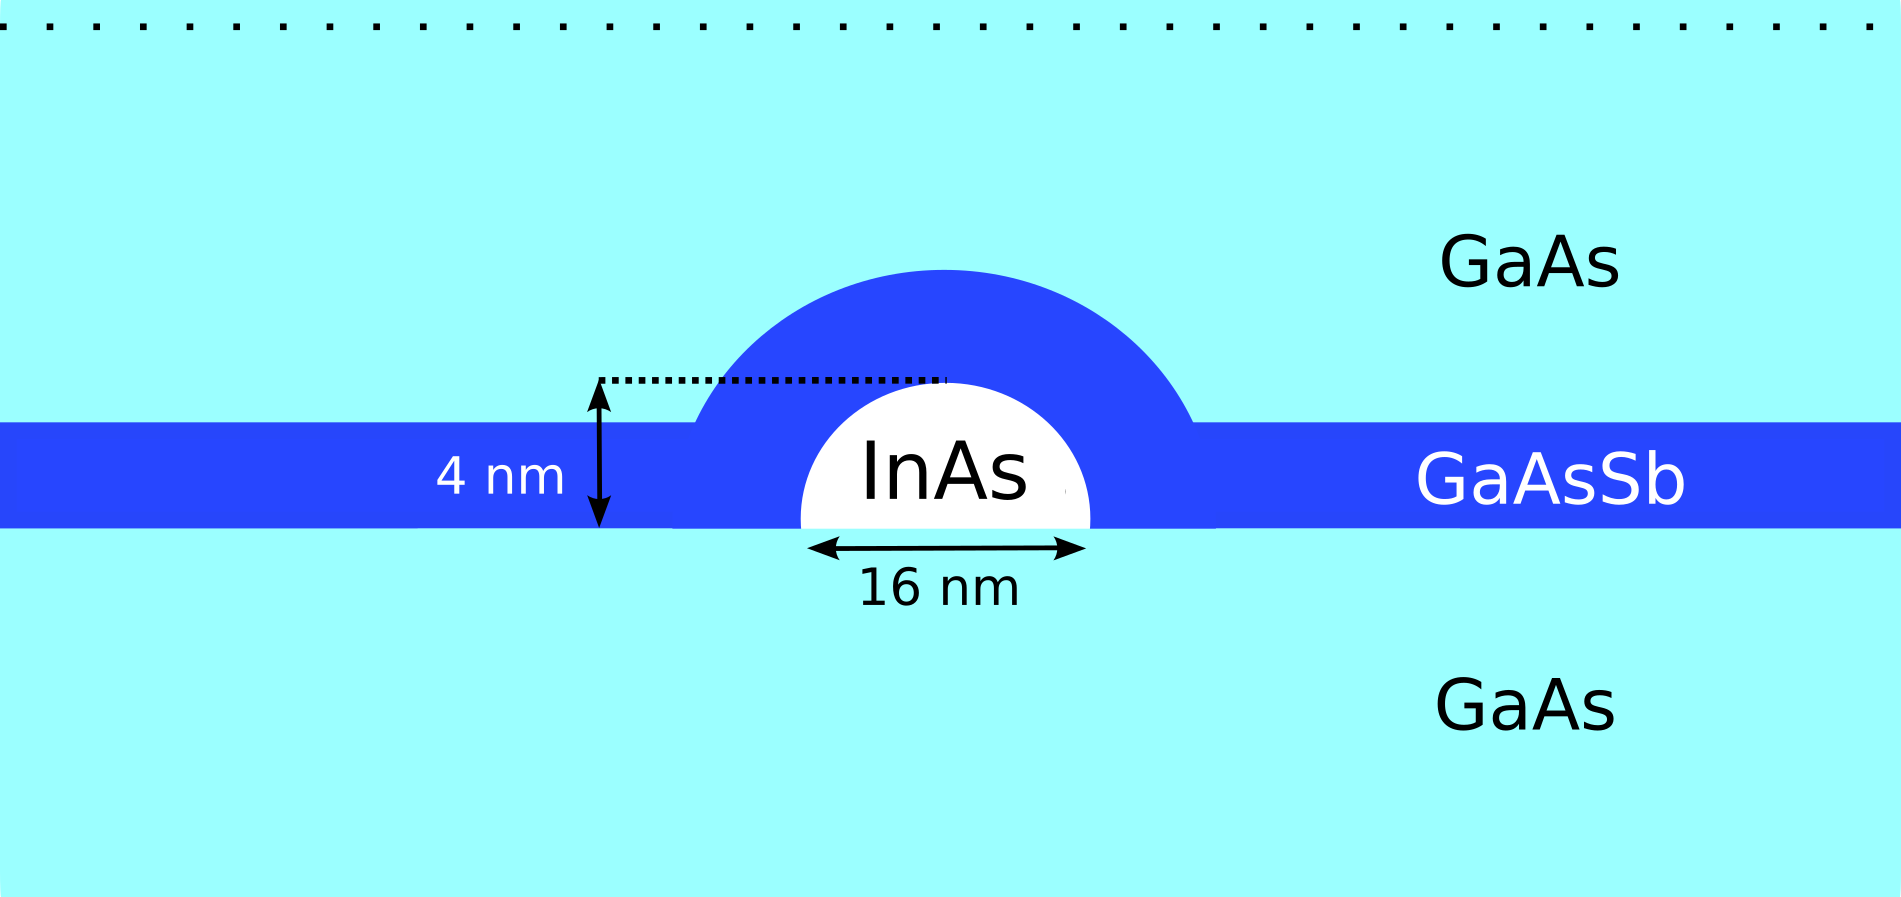
\includegraphics[width=1\linewidth]{/TEM/structure}
	\caption{Studied set of samples, $S_\mathrm{w/o}$ represents structure without QDs, $S_\mathrm{with}$ and $S_\mathrm{cap}$ are samples with In$_{1-x}$Ga$_{x}$As$_y$Sb$_{1-y}$ QDs, $S_\mathrm{cap}$ is, moreover, GaSb capped. }
	\label{fig:TUstructure}
\end{figure}

\begin{table}
	\centering
	\caption{Labels and studied sample differences.}
	%\begin{tabularx}{0.9\textwidth}{ccccc}
	\begin{tabularx}{0.95\textwidth}{ccl}
		\toprule

		%growing name & our marking& \multicolumn{3}{c}{specification}\\ 
		sample name & label& \multicolumn{1}{c}{specification}\\ 		
		\midrule
		\midrule
		%TU 12027& $S_\mathrm{w/o}$ & 5ML GaAs& &\\
		TU 12027& S$_\mathrm{w/o}$ & 5ML GaAs\\
		%TU 12040& $S_\mathrm{with}$ & 5ML GaAs,& 0.51ML In$_{1-x}$Ga$_{x}$As$_y$Sb$_{1-y}$&\\
		TU 12040& S$_\mathrm{with}$ & 5ML GaAs, 0.51~ML In$_{1-x}$Ga$_{x}$As$_y$Sb$_{1-y}$ QDs\\
		%TU 12021 & $S_\mathrm{cap}$ & 5ML GaAs,& 0.51ML In$_{1-x}$Ga$_{x}$As$_y$Sb$_{1-y}$,& GaSb cap\\
		TU 12021 & S$_\mathrm{cap}$ & 5ML GaAs, 0.51~ML In$_{1-x}$Ga$_{x}$As$_y$Sb$_{1-y}$ QDs, GaSb cap\\
		\bottomrule
	\end{tabularx}\label{tab:samples}
\end{table}


% http://nano.ceitec.cz/high-resolution-scanning-transmission-electron-microscope-fei-titan-themis-60-300-cubed/

We have studied the material composition of the sample S$_\mathrm{cap}$ by transmission electronic microscopy (TEM) with an add-on energy-dispersive X-ray (EDX) detector (SUPER-X EDX detector was used). These measurements were performed at the high resolution TEM FEI Titan Themis at CEITEC Brno. The TEM image of the whole sample and EDX emission spectrum are attached in appendix~\ref{chapter:appendix_TEM}.

In Fig.~\ref{fig:TEM}, cross-sectional TEM micrograph and graphs from simultaneously measured EDX spectra for sample S$_\mathrm{cap}$ are presented. EDX spectrum is collected along the orange dashed line and averaged in the yellow boundary area. In the atomic fraction graph we show material composition on the sample as a function of horizontal position for all constituents (Ga, P, As, In, Sb). In the range between 30 and 40~nm in the cut the fractions of In, As and Sb composition (elements, which are expected only in QDs area) dramatically increase in comparison with the concentration of 0.8~\% seen in the remainder of the sample. In the same range, we can see a decrease in phosphorus concentration at the expense of GaP. The layer where In concentration is higher than 0.8~\% we regard as QD area and its thickness is found to be of 5.8~nm with truncated-pyramid shape QDs with a base length of about 15~nm and a height of 2.5~nm. 
\begin{figure}
	\centering
	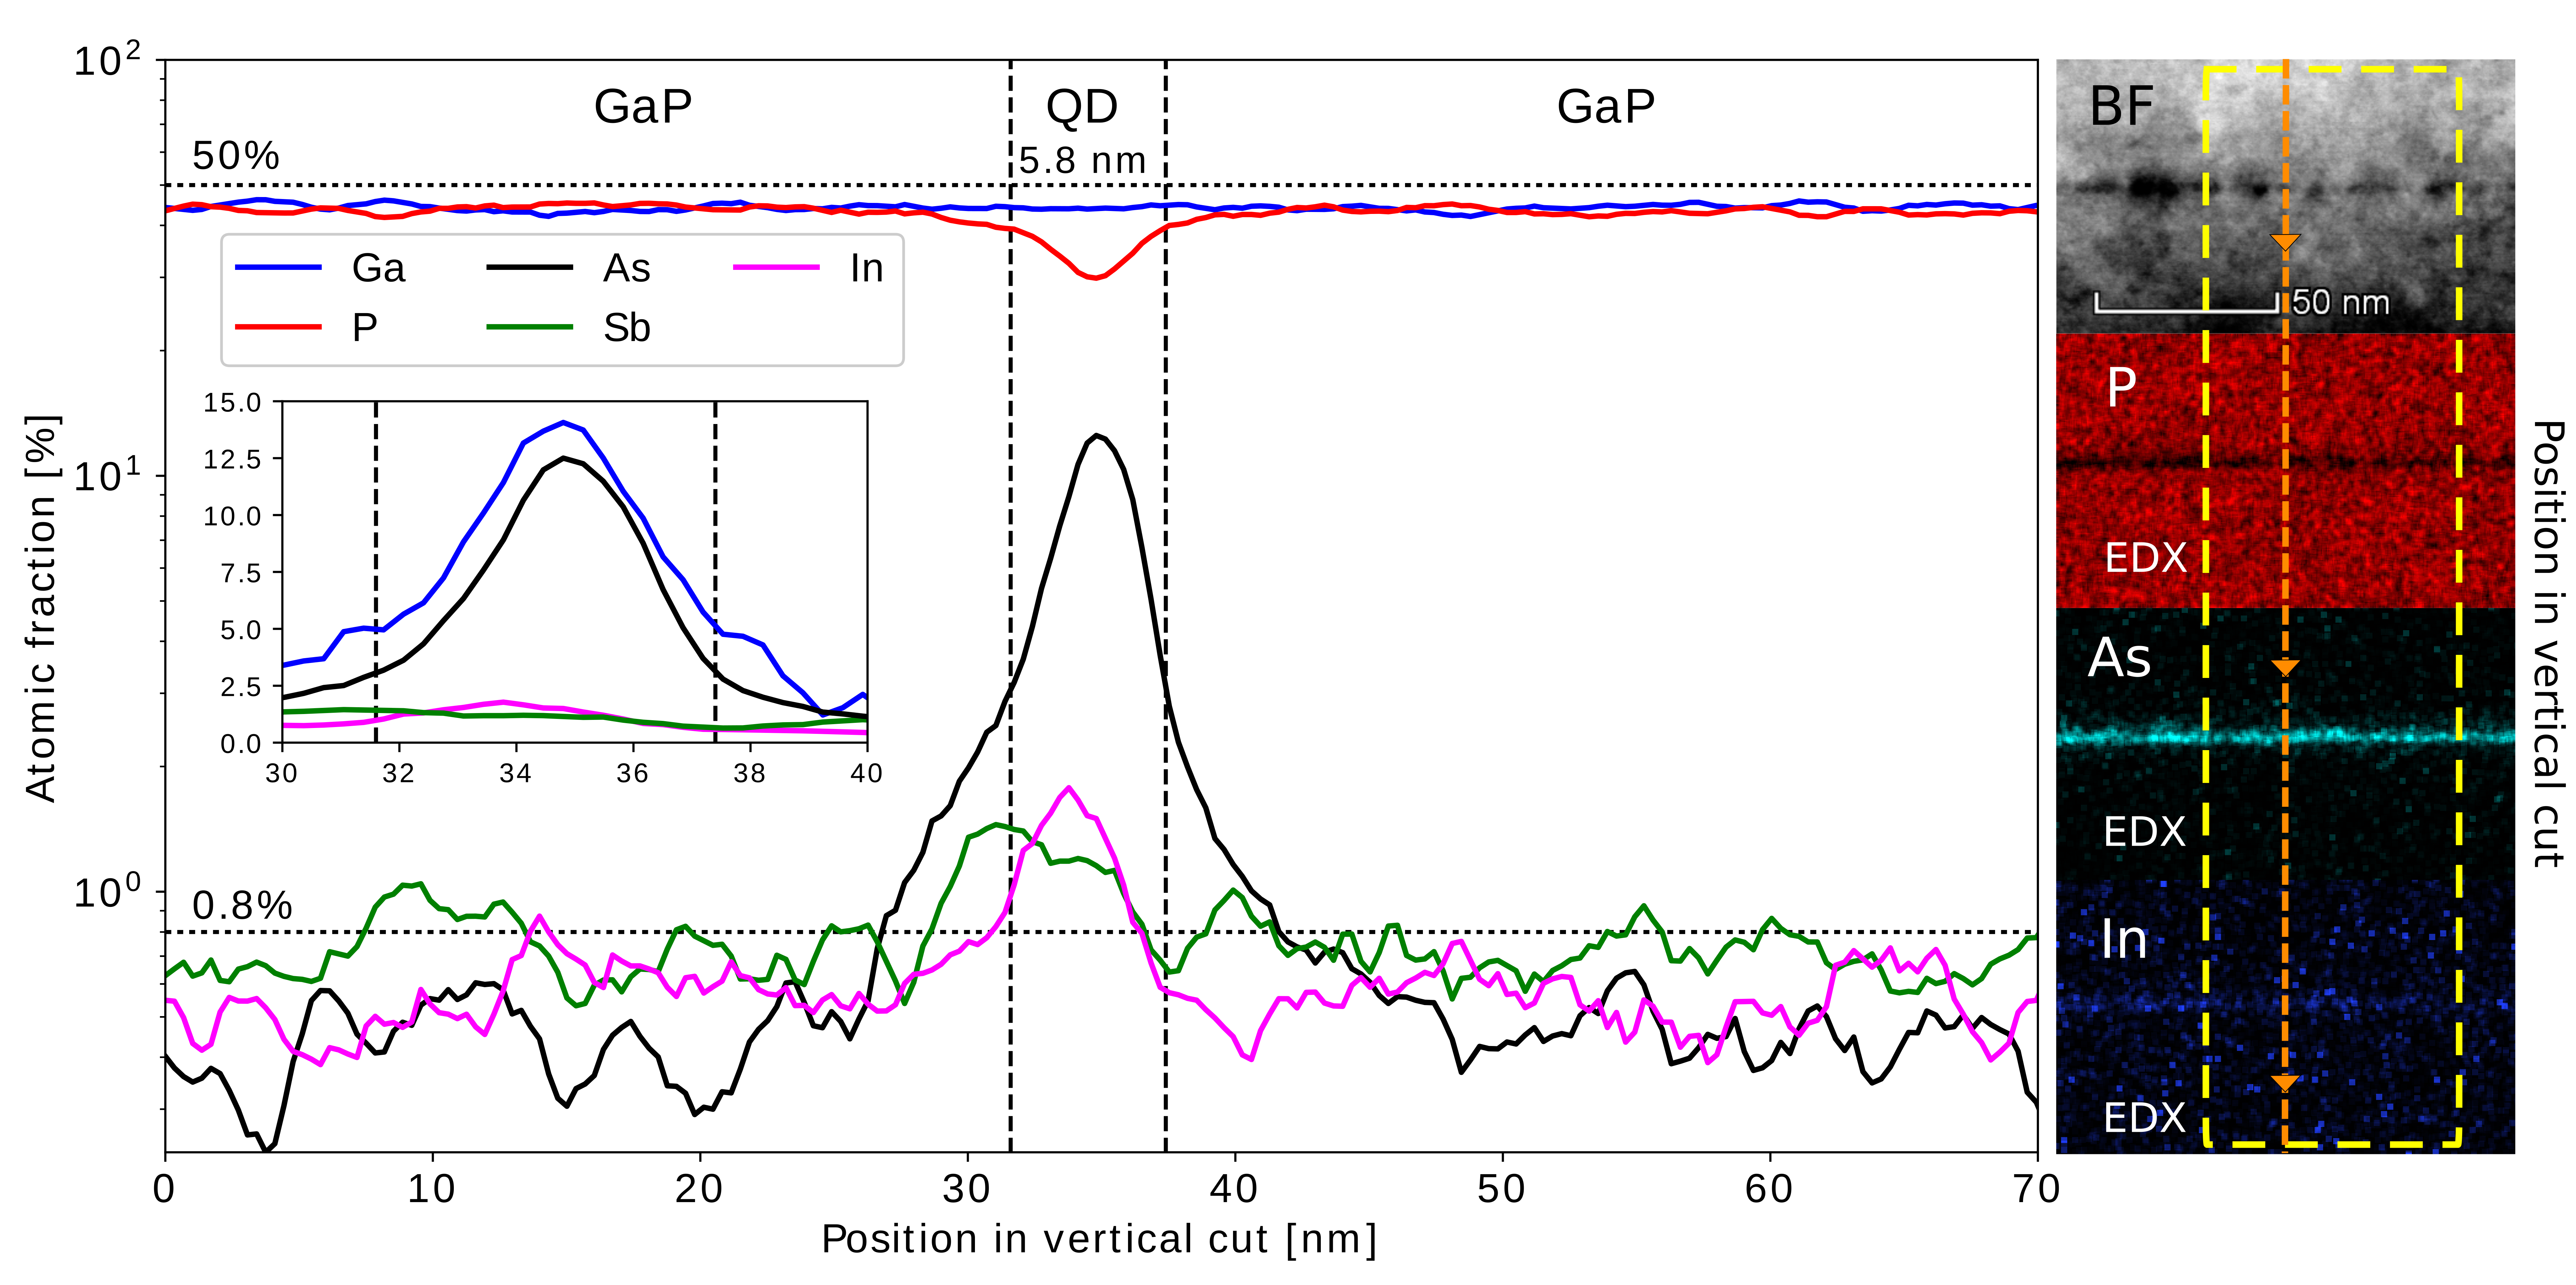
\includegraphics[width=1\linewidth]{/TEM/koncentrace_final_mapa2_QDinset}
	\caption{The atomic fraction vs. position in the vertical cut for all elements present in sample S$_\mathrm{cap}$ measured by EDX detector along the orange line in the right panel and averaged in the area circumferenced by the yellow broken curve. In QD area, i.~e., between the vertical positions of 30 and 40~nm in the cut, a substantial increase of In, As, Sb (compounds only in QD structures) and decrease of P (P is out of the QD structures) are observed. The inset shows the composition solely in the QD region. The column on right-hand side represents from top to bottom: cross-section TEM image of S$_\mathrm{cap}$ taken under strong-beam bright field condition using the (200) reflection perpendicular to the growth direction; and three EDX images measured at the same time as TEM measurements -- red one for P, white in As and purple in In.}
	\label{fig:TEM}
\end{figure}

We use the EDX data to estimate the concentration of individual elements in quaternary QD structure. Assuming that all phosphorus is bound in GaP, the concentration of Ga can be divided into Ga concentration in GaP $C_\mathrm{GaP}$ and in QD area $C_\mathrm{Ga}^\mathrm{QD}$ as
%
\begin{eqnarray}
C_\mathrm{Ga}=C_\mathrm{GaP}+C_\mathrm{Ga}^\mathrm{QD}=C_\mathrm{P}+C_\mathrm{Ga}^\mathrm{QD},
\end{eqnarray}
%
where $C_\mathrm{i}$ for $i \in \{\mathrm{Ga}, \mathrm{P}\}$ is the measured concentration of Ga and P. We assume the composition of our QDs in the form of In$_{1-x}$Ga$_{x}$As$_y$Sb$_{1-y}$, thus, we can calculate effective concentration in QD area as
%
\begin{eqnarray}
x=\frac{C_\mathrm{Ga}^\mathrm{QD}}{C_\mathrm{Ga}^\mathrm{QD}+C_\mathrm{In}^\mathrm{QD}},\qquad
y=\frac{C_\mathrm{As}^\mathrm{QD}}{C_\mathrm{As}^\mathrm{QD}+C_\mathrm{Sb}^\mathrm{QD}}.
\end{eqnarray}
%
Given the assumption that In, Ga and Sb are only in QD area, we can replace the concentration in this region by data from EDX. Finally, we give the estimation of $x$ and $y$ which we use in 8-band $\mathbf{k\cdot p}$ calculations of $x=84-93.5~\%$ and $y=68-91.5~\%$, see Fig.~\ref{fig:concentration_estimation}.


\begin{figure}
	\centering
	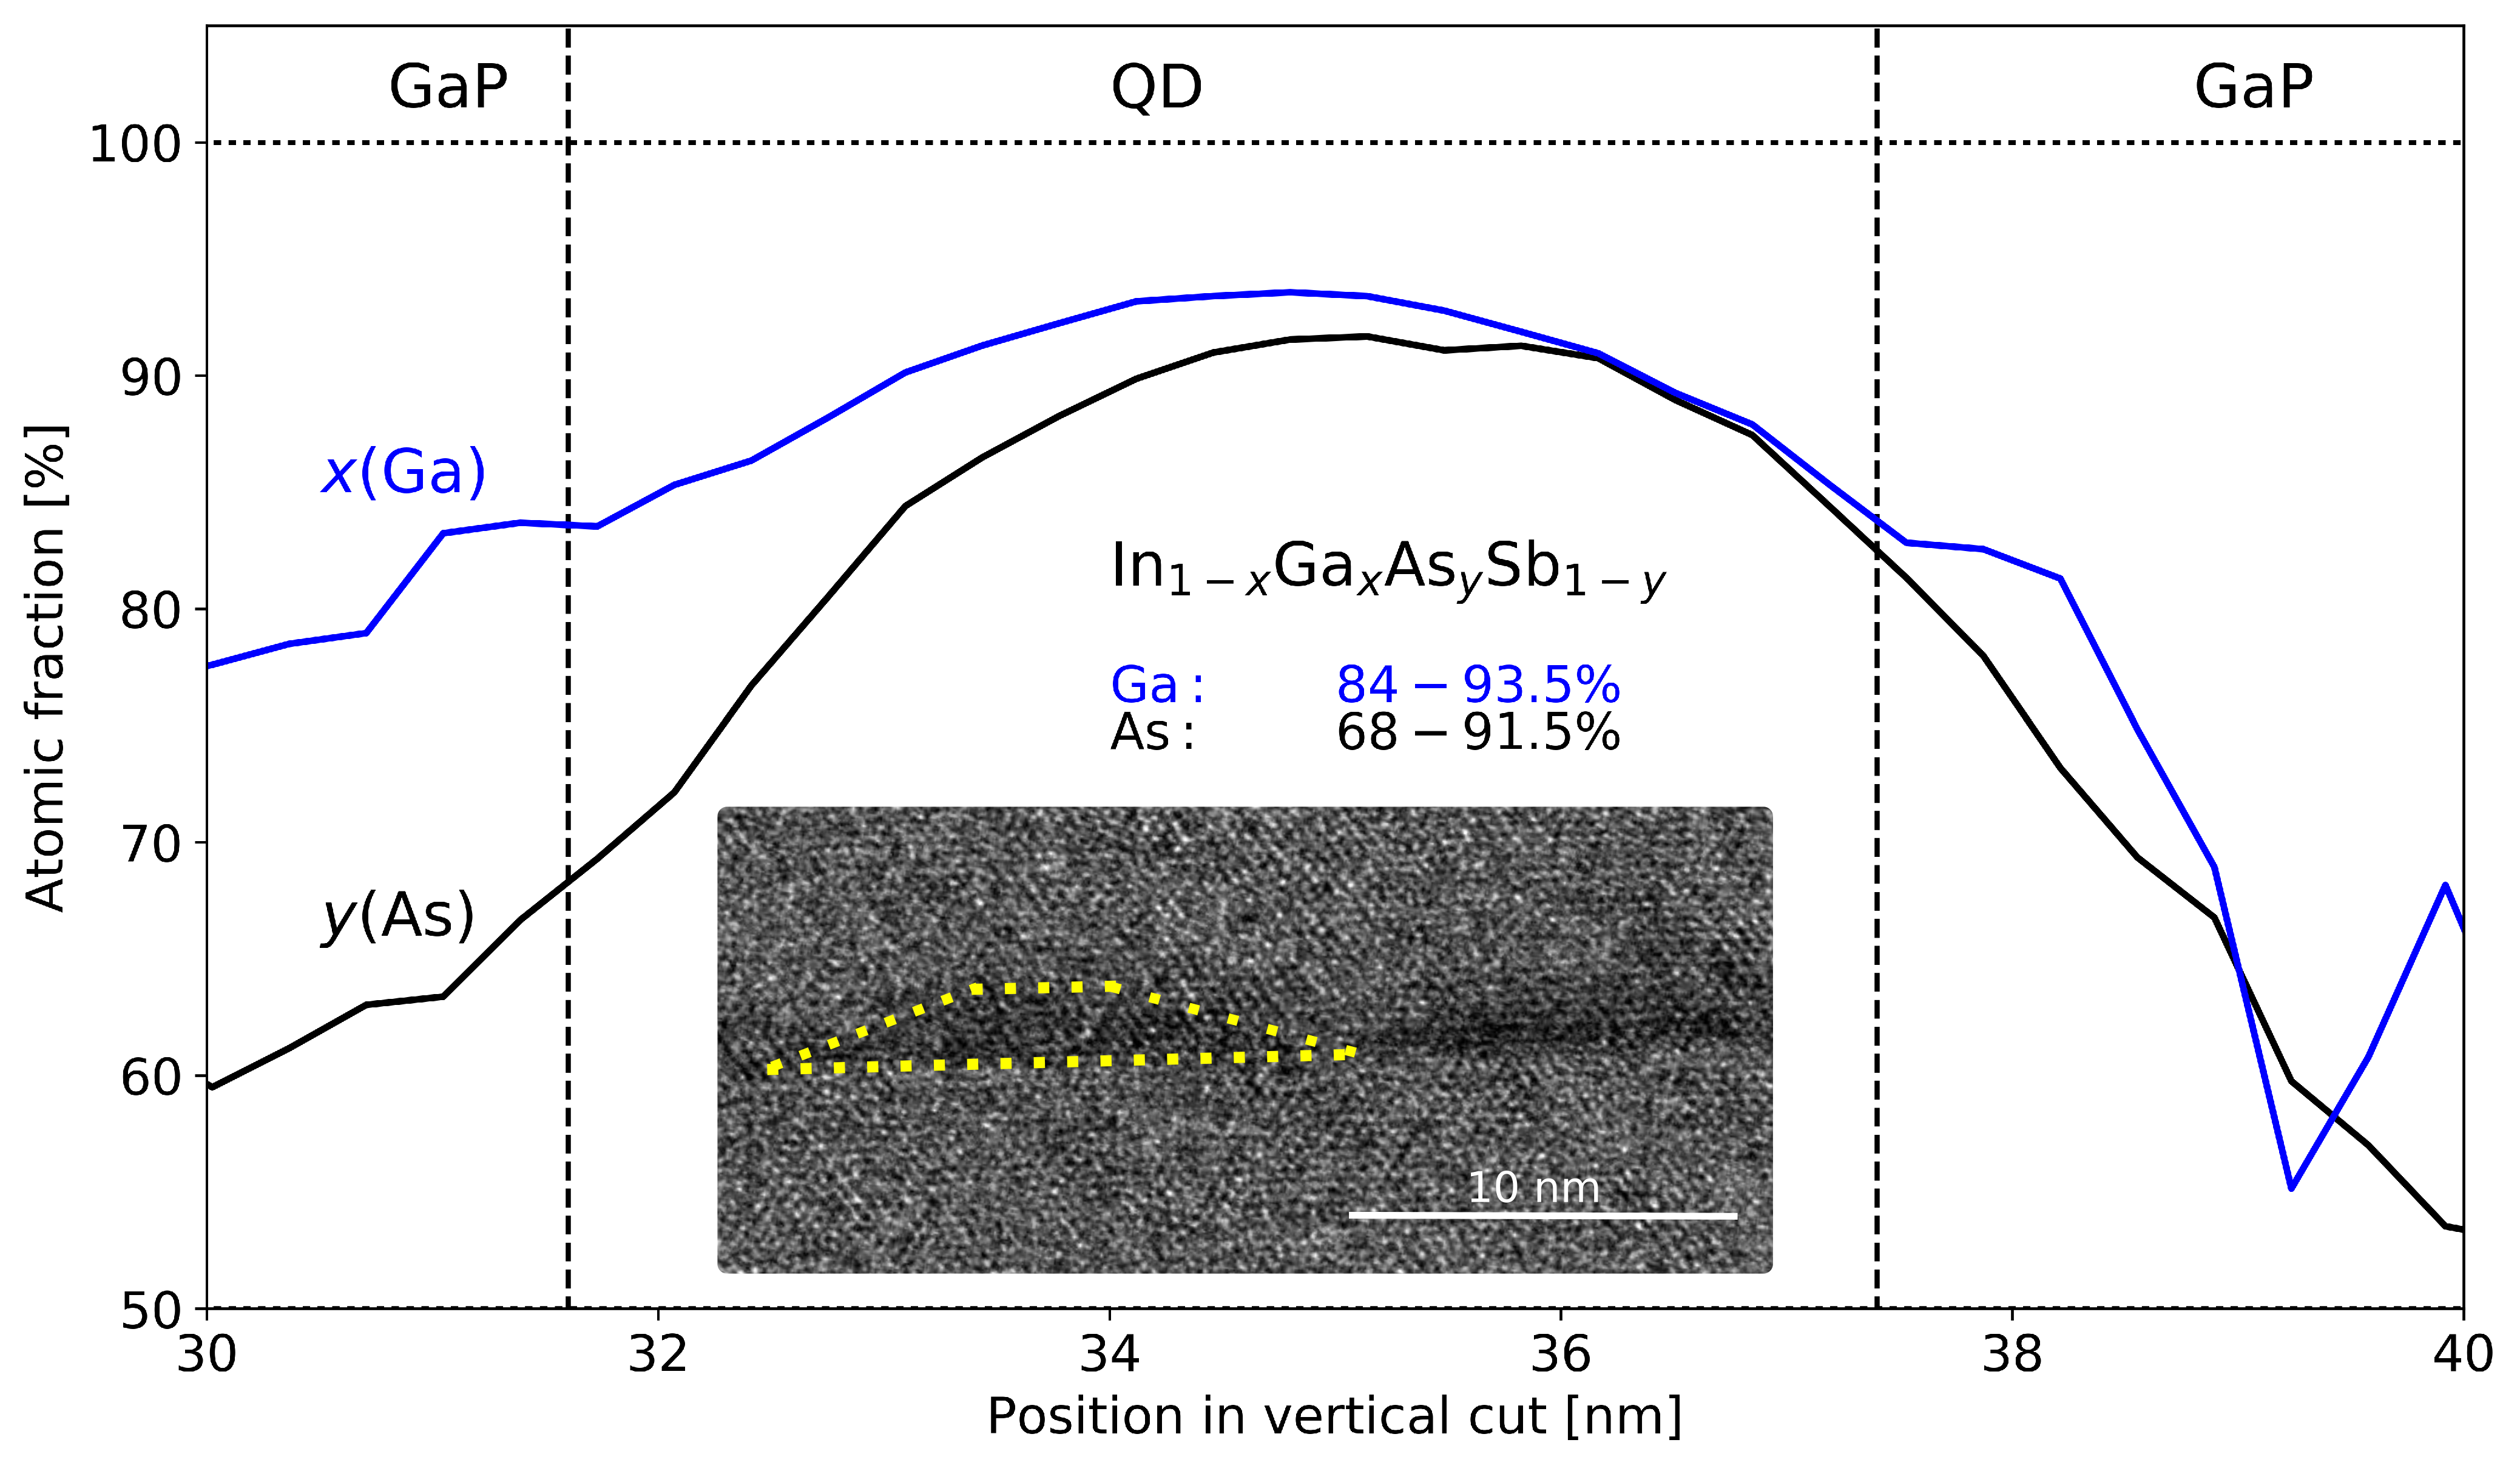
\includegraphics[width=0.85\linewidth]{/TEM/koncentrace_pro_nn} %rez_QD_konc_xy_bez}
	\caption{The estimated composition of QD area for sample S$_\mathrm{cap}$. We assume Ga and As concentration to be in the ranges of 84--93.5~\% and 68--91.5~\%, respectively. In inset we show the HRTEM image of a truncated-pyramid QD.}
	\label{fig:concentration_estimation}
\end{figure}

{\color{blue}{To sum up TEM and EDX results, our samples contain In$_{1-x}$Ga$_{x}$As$_y$Sb$_{1-y}$ QDs of shape like truncated pyramid of base length of 15~nm and height 2.5~nm with a higher estimated concentration of Ga ($x=84-93.5~\%$) and As ($y=68-91.5~\%$).}}
%\clearpage

\section{Estimation of hydrostatic strain in GaAs layer}
For estimation of a hydrostatic component of strain we have performed room temperature Raman measurements of our samples. These measurements were obtained using NT-MDT spectrometer with a 100$\times$/0.7~NA long working length objective and 532~nm laser. The scattered light was dispersed using a 1800~groove/mm grating and detected by a thermoelectrically cooled Si CCD camera. The spectra were recorded in $z(xy)z$ backscattering geometry.

Measured signals were fitted by the sum of 3 Lorentzian curves.
Let us focus on Raman signal around 290~cm$^{-1}$ where TO phonon of strained GaAs wells (QWs) for our QDs samples is expected. Fig.~\ref{fig:raman} indicates $\sim$19~cm$^{-1}$ shift of TO phonon for our QD samples compared to bulk material. Using a model given in Ref.~\cite{Montazeri_Nano2010} we can use that shift to estimate the value of hydrostatic strain $\epsilon_{xx}$ 
\begin{equation}
k_\mathrm{TO}^2 = k_\mathrm{TO,B}^2 + (p+2q)\epsilon_{xx},
\end{equation}
where $k_\mathrm{TO}$ and $k_\mathrm{TO,B}$ are the Raman shifts of TO GaAs mode of strained and bulk GaAs, and $p$ and $q$ are phonon deformation potentials taken from Ref.~\cite{Cerdeira_PRB1972}.

The measured shifts of TO mode for $S_\mathrm{w/o}$ correspond to $\epsilon_{xx}=-0.032$, for $S_\mathrm{with}$ to $\epsilon_{xx}=-0.026$,  and for $S_\mathrm{cap}$ we find $\epsilon_{xx}=-0.030$, which is in good agreement with the predicted hydrostatic strain component $\epsilon_{xx}=-0.034$ by the $\mathbf{k \cdot p}$ calculations, see Fig.~\ref{fig:raman_theory_wo}. %approximately three times less than predicted hydrostatic strain component by the $\mathbf{k \cdot p}$ calculations, see Fig.~\ref{fig:raman_theory_wo}.
\begin{figure}
	\centering
	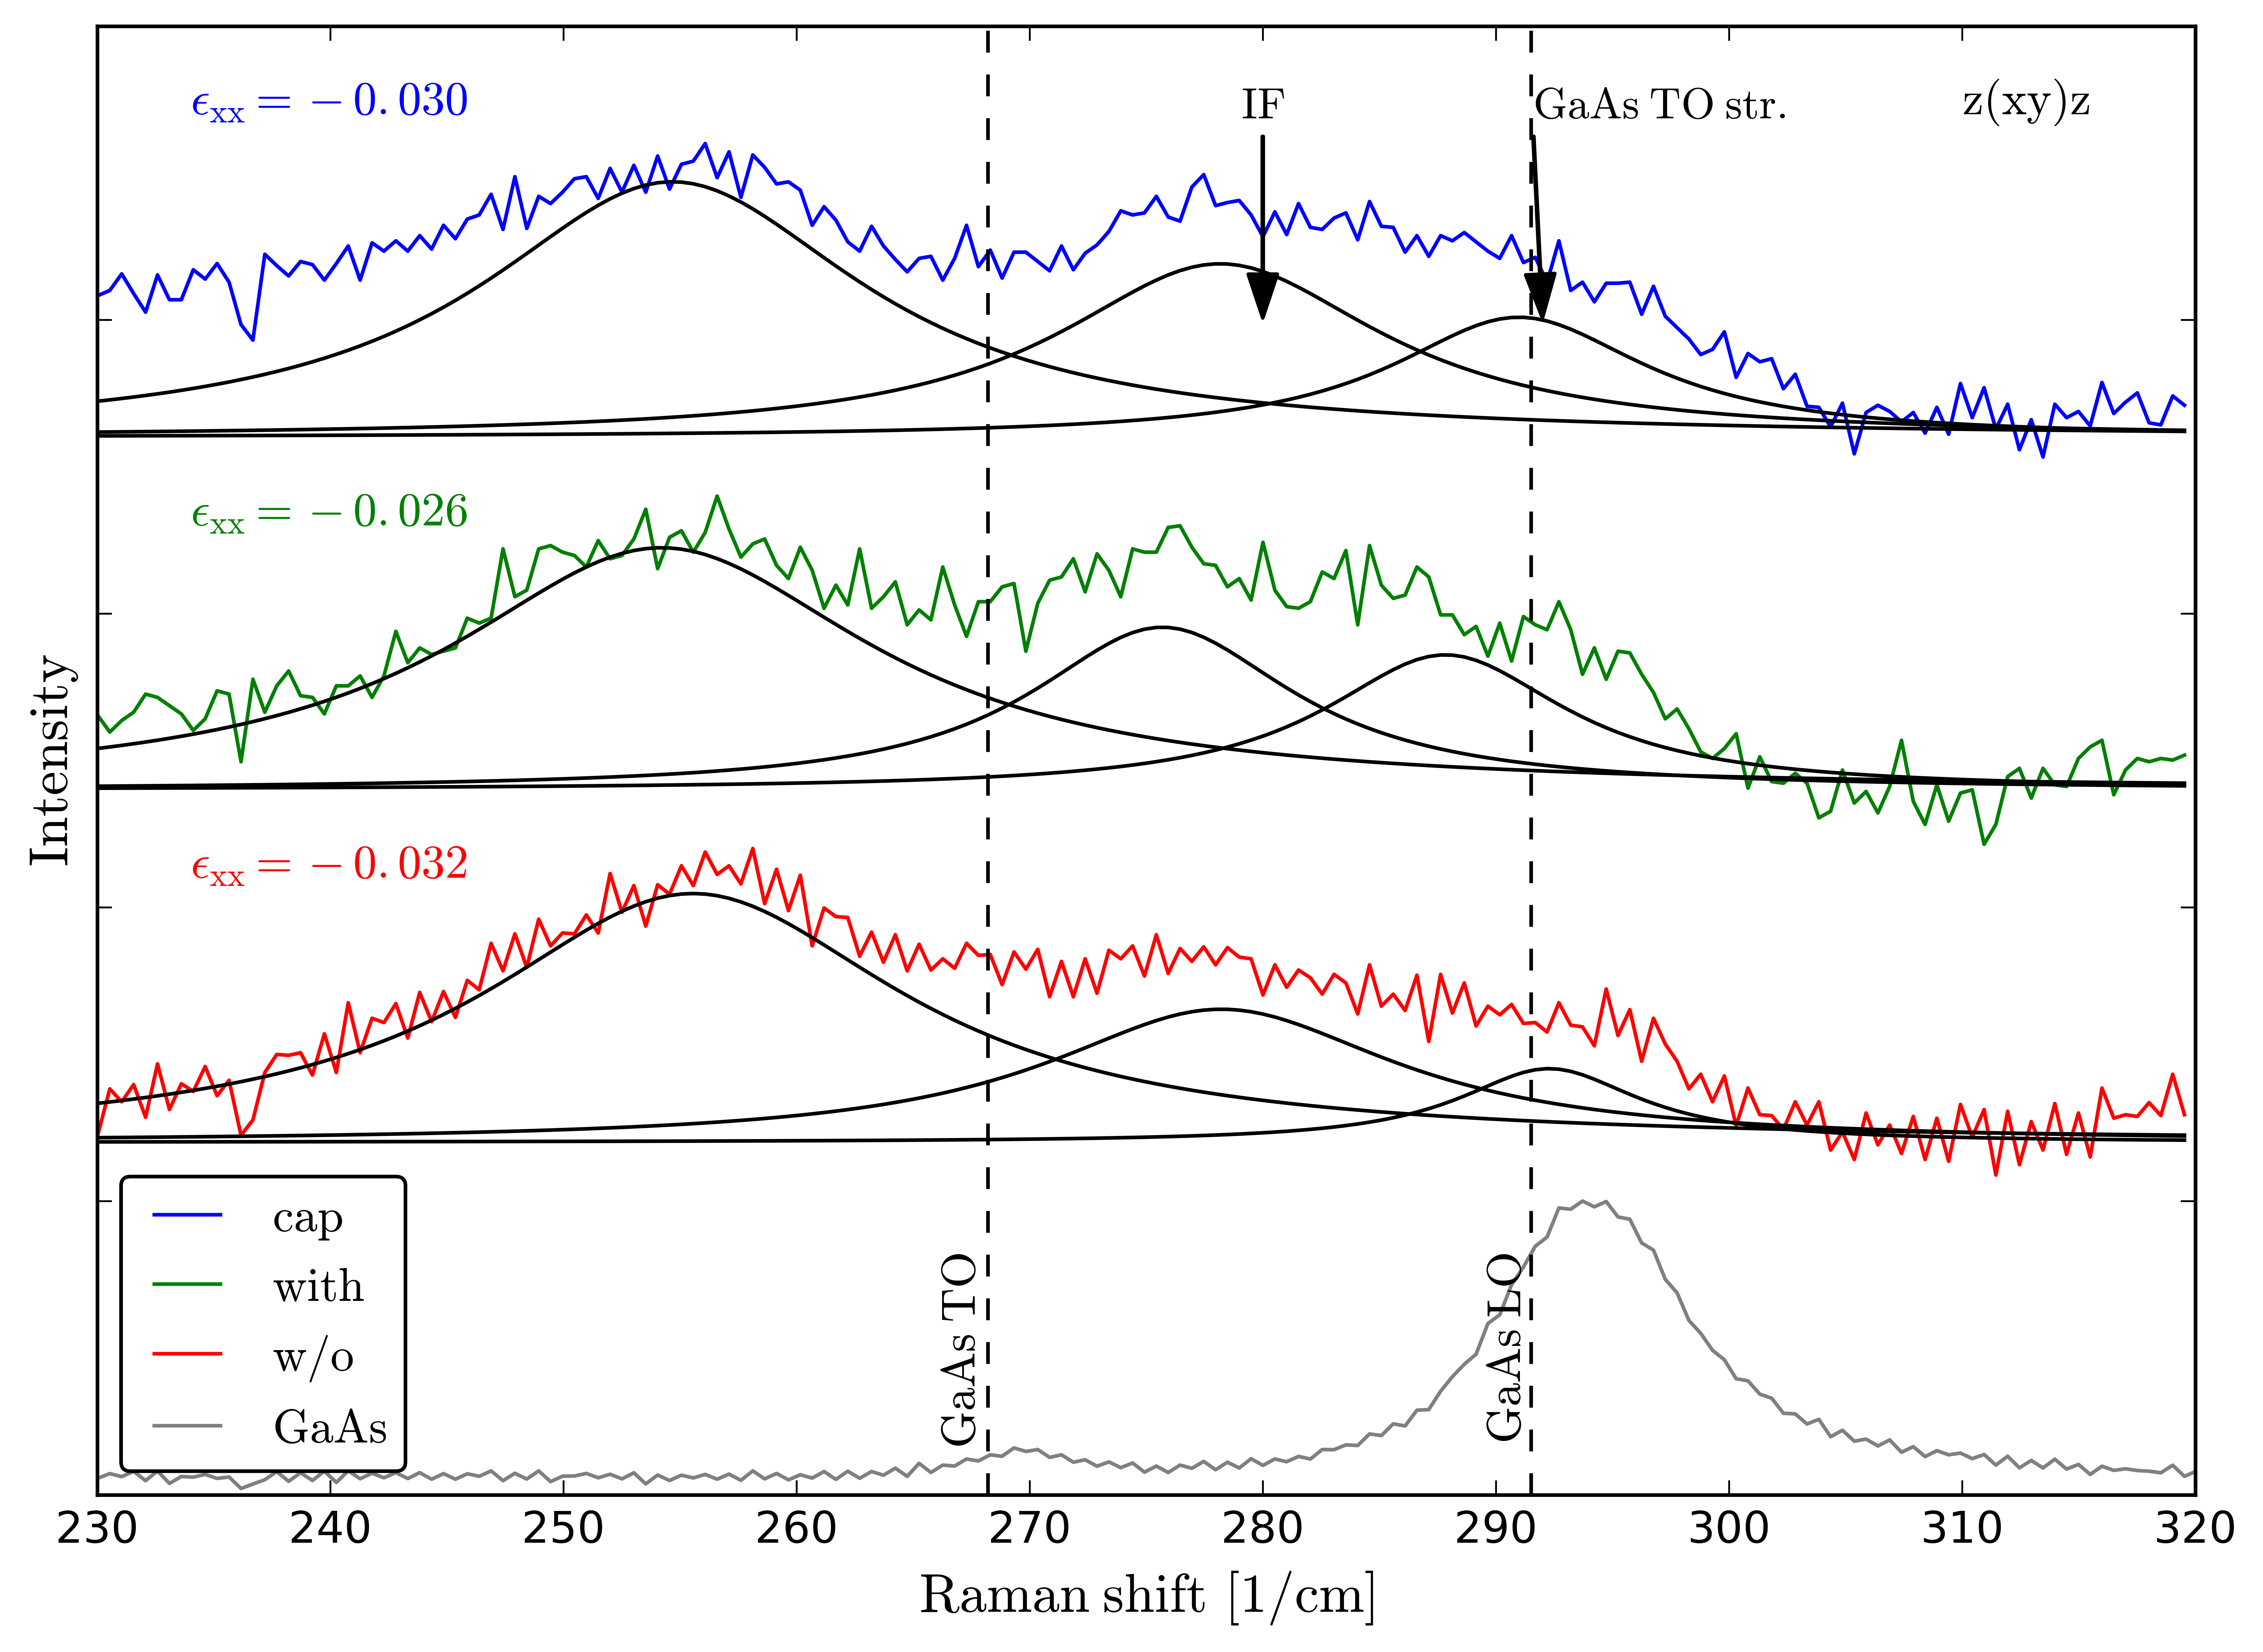
\includegraphics[width=0.85\linewidth]{/raman/Raman_TUB_and_GaAs_enlg_230_to_320_fit}
	\caption{Raman spectra of samples w/o QDs $S_\mathrm{w/o}$ (red), with QDs $S_\mathrm{with}$ (green) and capped QDs $S_\mathrm{cap}$ and bulk GaAs (grey). The dashed lines show reference GaAs TO and LO modes~\citep{Esther_Nanotech2013}. Calculated hydrostatic strain components $\epsilon_{xx}$ are presented in insets of the figure. A label IF corresponds to interface Raman band.}
	\label{fig:raman}
\end{figure}

\begin{figure}
	\centering
	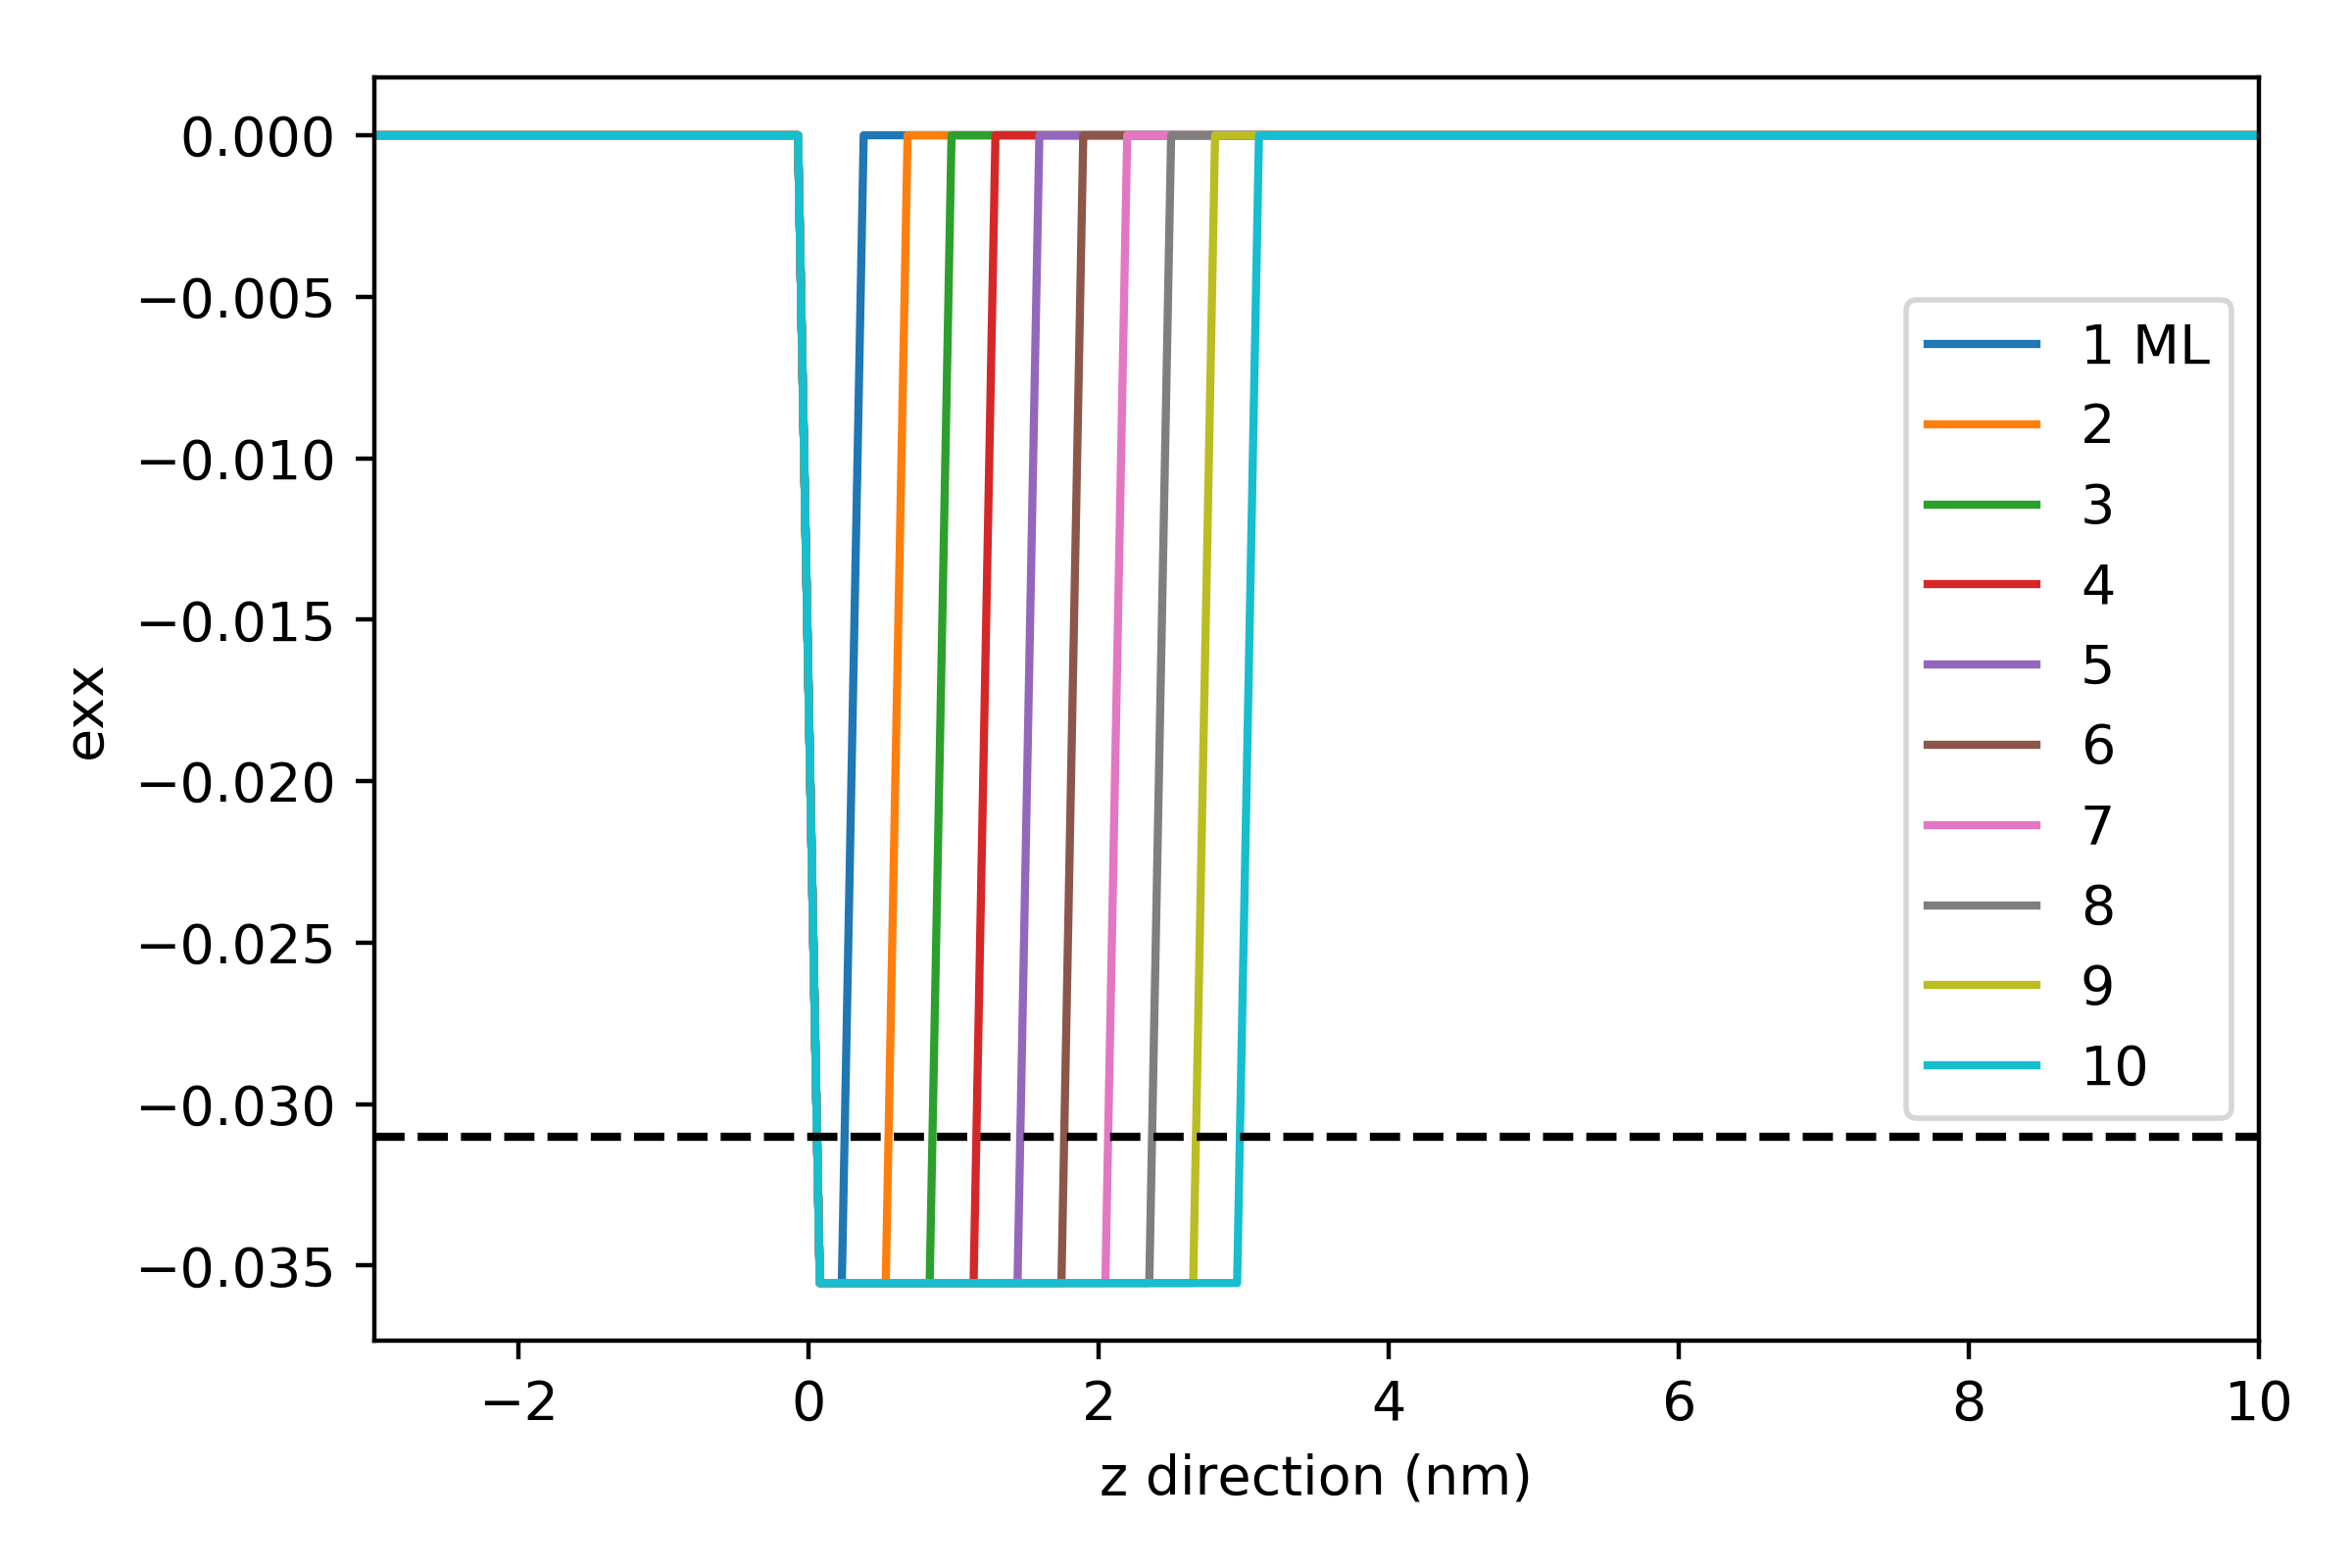
\includegraphics[width=0.85\linewidth]{/raman/eyy_vs_ML}
	\caption{Hydrostatic strain $\epsilon_{xx}$ calculated as a function of GaAs layer thickness in the sample $S_\mathrm{w/o}$. The experimental value is represented by a dashed horizontal curve. The calculations were made by the supervisor.}
	\label{fig:raman_theory_wo}
\end{figure}

{\color{blue}{The analysis pointed to change of hydrostatic strain $\epsilon_{xx}$ connected with partial relaxation of strained GaAs layer due to growth QDs. The addition of the GaSb capping layer is likely to increase $\epsilon_{xx}$ in GaAs layer again.}}


\clearpage


\section{Experimental setup for photoluminescence measurements}
The PL measurements were performed using standard PL setup. The samples were positioned in the cryostat, cooled to 15~K and pumped by a laser diode with the wavelength of 405~nm and focused to 0.05~mm$^2$ large spot size. The emitted emission signal was dispersed by a 1200~grooves/mm ruled grating designed to the wavelength of 750~nm and synchronously detected by a Si avalanche photodiode (APD). We have performed the following PL experiments: (i) in intensity dependent measurements the laser power was varied by a neutral density (ND) filter over more than 4 orders of magnitude, (ii) in the temperature resolved PL temperature was changed from 15~K to room temperature, but for our samples and given integration time (0.3~s per one wavelength) we have not detected any PL signal at 300~K, (iii) the polarization of the PL was analyzed by a rotating achromatic half-wave retarder followed by a fixed linear polarizer.

In time-resolved experiments we have used laser with wavelength of 405~nm focused on 0.06~mm$^2$ area with pulse-width of 60~ps; emitted PL spectrum was dispersed again by 1200~grooves/mm ruled grating and detected by a Si APD. We have performed the following TRPL experiments: (i) intensity resolved TRPL was measured at 15~K in 200~ns temporal window with resolution around 800~ps; the pumping power density was tuned by a ND filter in a range of 0.1--0.7~W/cm$^2$. The repetition rate of the laser was 5~MHz. (ii) In temperature resolved TRPL a temperature was changed on a range 15--150~K, the temporal window was modified to maximize the resolution from 200~ns for lower temperature to 25~ns for higher temperature. Tuning the temporal window is connected with changes in repetition rate, which was varied between 5 (for the temporal window 200~ns) and 80~MHz (for 25~ns).

Both experimental setups are schematically depicted in~Fig.~\ref{fig:Madrid_setup}.
\begin{figure}
	\centering
	\includegraphics[width=1\linewidth]{/PL/setup}
	\caption{Schematic of the (a) PL and (b) TRPL measurement setup. The sketch of the TRPL setup is motivated by Ref.~\citep{TRPL_setup}.}
	\label{fig:Madrid_setup}
\end{figure}


\newpage
\section{Photoluminescence measurements}

The homogeneity of samples was tested by performing PL measurements on different spots of them. The results of that for each sample (distinguished by the type of the curve) and for various samples (different color) are depicted in the Fig.~\ref{fig:PL_homogenity}. We can see that samples are rather spatially homogeneous, hence our measurements might be considered as reproducible for each sample. %it is not necessary measured PL and TRPL in the same time. 

Let us look at the emission around the energy of 1.8~eV. Firstly, we compare substrate emission in this spectral range with signal from our samples. We clearly see a broader band which is approximately 70~times smaller than emission from our samples so it seems reasonable to neglect this band. For sample $S_\mathrm{w/o}$ we show PL with two maxima located at 1.83 and 1.86~eV, respectively. The PL signal of samples with QDs is shifted to smaller energies: the maxima are located at 1.78~eV for $S_\mathrm{with}$ and 1.74~eV for $S_\mathrm{cap}$. Finally, let us notice that the PL from $S_\mathrm{with}$ is twice stronger compared to other samples.
\begin{figure}
	\centering
	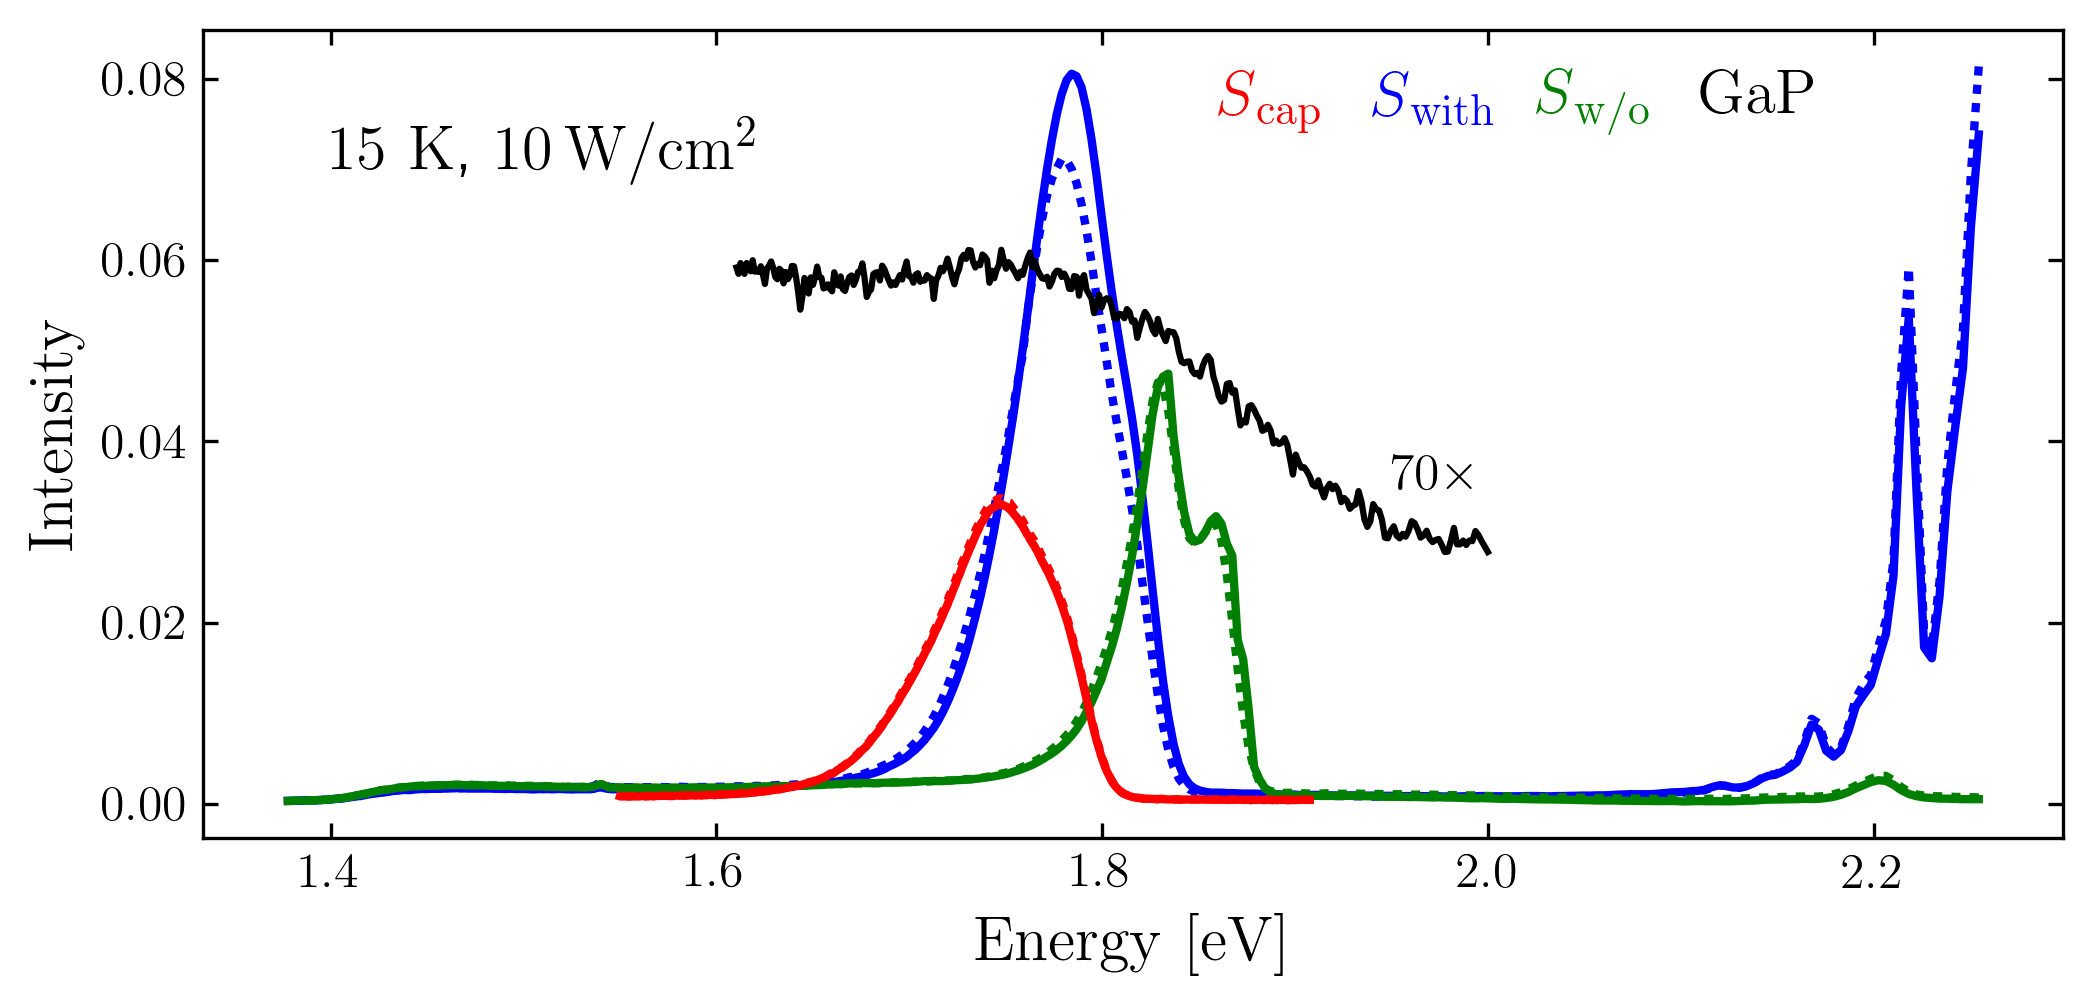
\includegraphics[width=1\linewidth]{/PL/all__IntensityVSen_GaP}
	\caption{PL for samples $S_\mathrm{w/o}$ (green lines), $S_\mathrm{with}$ (blue) and $S_\mathrm{cap}$ (red) measured at 15~K and with laser power of 10~W/cm$^2$ on several places on samples (different curve types). PL from our samples is compared with emission from GaP substrate multiplied by a factor of 70 (black).}
	\label{fig:PL_homogenity}
\end{figure}

%Pridano 
{\color{blue}{Based on TEM results, $\mathbf{k \cdot p}$ calculations of In$_{1-x}$Ga$_{x}$As$_y$Sb$_{1-y}$/GaAs/GaP truncated pyramid QD with the base of 15~nm and height 2.5~nm were calculated by the supervisor for varying As and Ga content in QD. The results obtained by $8\times 8~\mathbf{k \cdot p}$ for electron in $\Gamma$-point and $1\times 8~\mathbf{k \cdot p}$ for $L$ and $X$ bands are shown in Fig.~\ref{fig:Gamma_L_reverse}. Interestingly, around emission energy 1.8~eV for $x=0.85$, $y=0.90$ the $L$ and $\Gamma$ bands swap.}}
		

\begin{figure}
	\centering
	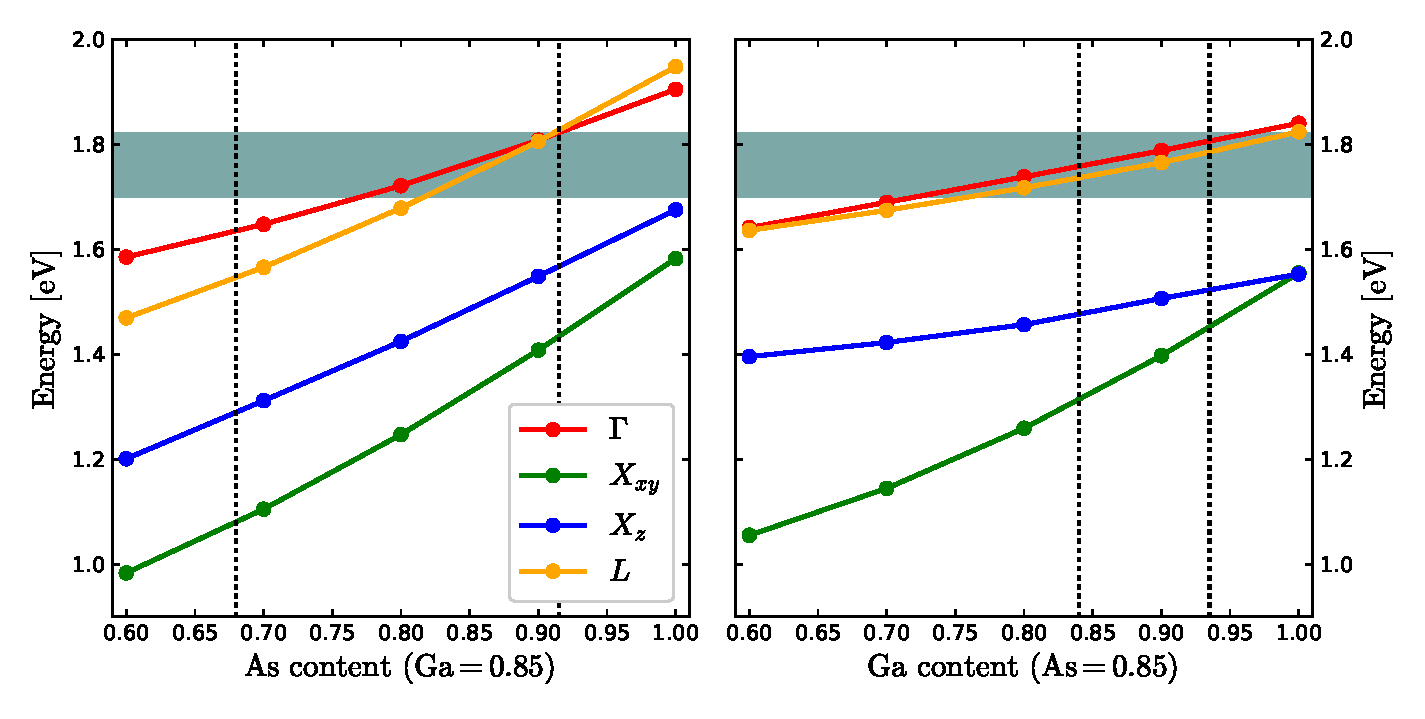
\includegraphics[width=0.9\linewidth]{/TUB_theory/swap_bands}
	\caption{{\color{blue}{Emission energy from various energy bands calculated by $\mathbf{k \cdot p}$ method for truncated pyramid shape QD of base length 15~nm and height 2.5~nm as a function of material content in dot body. In left panel are results for fix Ga ($x=0.85$) and varying As concentration. In right panel is reverted situation, i.~e., fix As ($y=0.85$) and varying Ga. Vertical broken lines show the interval of obtained content from EDX analysis. The grey shadowed area represents the range of emission from our sample $S_\mathrm{with}$ and $S_\mathrm{cap}$.} }}
	\label{fig:Gamma_L_reverse}
\end{figure}
	

%konec pridano

\newpage
\subsection{Excitation intensity dependent PL}
\label{sec:intensity_PL_TU}
PL for each sample and excitation density $D$ was fitted by sum of three Gaussian curves and the individual bands corresponding to different optical transitions were studied. 

\subsubsection*{Sample without QDs $\mathbf{S_\mathrm{w/o}}$}
\label{Sec:PL_int_wo}
\begin{figure}
	\centering
	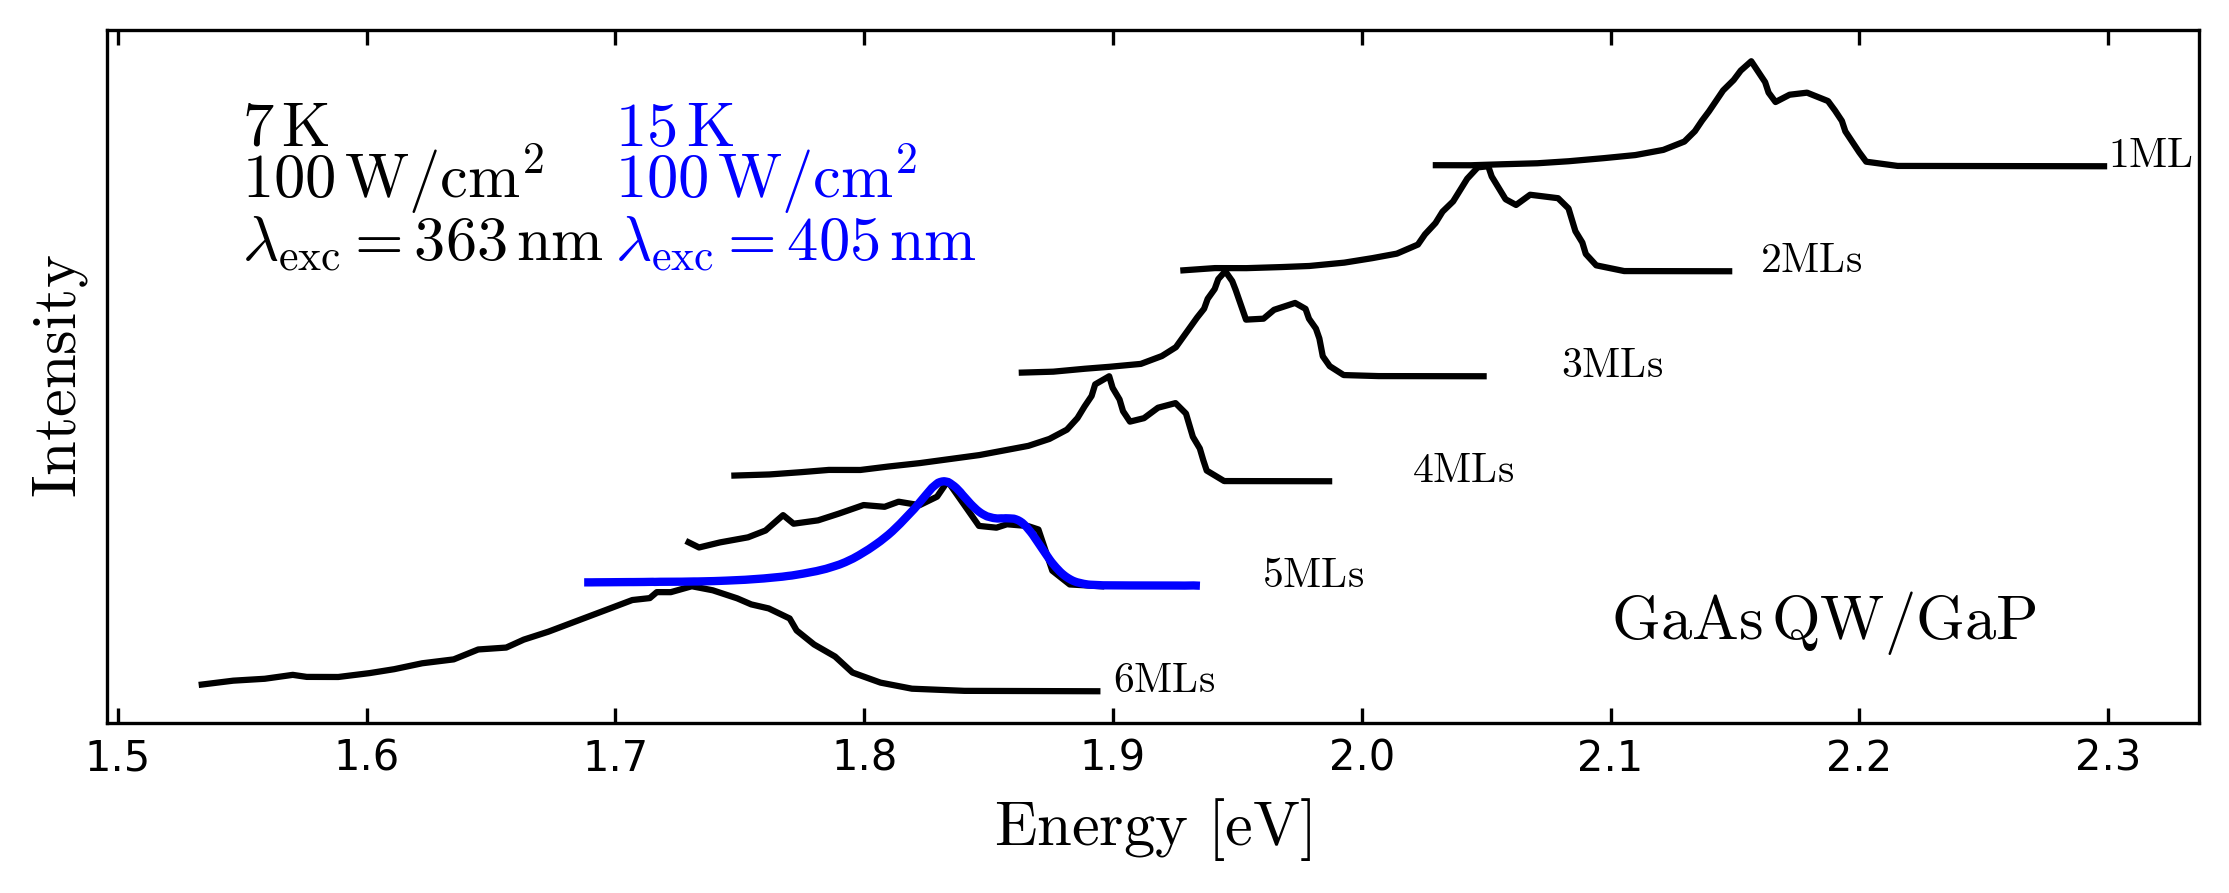
\includegraphics[width=0.9\linewidth]{/PL/12027_ref_GaAs_5ML_new}
	\caption{The comparison of the spectrum of $S_\mathrm{w/o}$ (blue) with set of samples with variable thickness taken from~Ref.~\citep{Prieto_APL1997} (black). The measurement temperature of 15~K (7~K), excitation wavelength of 405~nm (363~nm) in our (in Ref.~\citep{Prieto_APL1997}) were used. Excitation power density in both experiments was 100~W/cm$^2$. We can see a rather good match of sample $S_\mathrm{w/o}$ with 5ML thick GaAs QW from Ref.~\citep{Prieto_APL1997}.}
	\label{fig:12027_ref}
\end{figure}


\begin{figure}
	\centering
	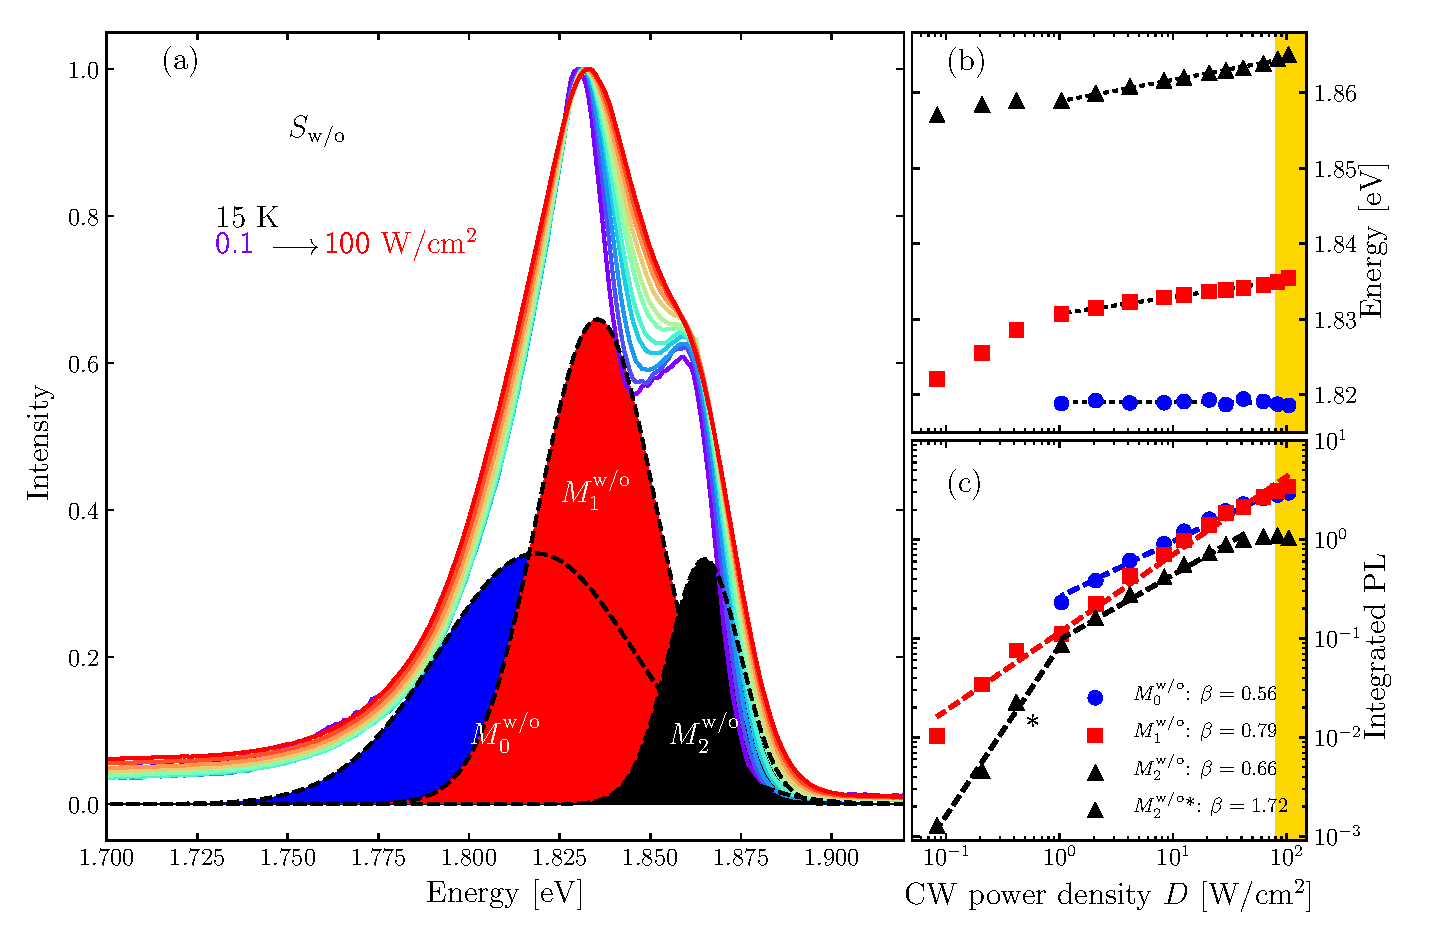
\includegraphics[width=0.9\linewidth]{/PL/intensity/12027_11011_norm_PL_int_satur}
	\caption{(a) PL spectra of $S_\mathrm{w/o}$ measured for several excitation densities in the range between 0.1 and 100~W/cm$^2$. The fit by the sum of three Gaussian curves is shown for 100~W/cm$^2$ and the individual bands are given by shaded areas: $M_0^\mathrm{w/o}$ (blue), $M_1^\mathrm{w/o}$ (red) and $M_2^\mathrm{w/o}$ (black). In (b) we show power dependence of the energy of individual bands and their fits by Eq.~(\ref{eq:PL_intmodel}) (dotted curves). Panel (c) depicts the integrated PL intensity of the bands in log-log scale and their fits by linear lines (broken lines), respectively. The slopes of the linear fit $\beta$ (exponent in linear scale) are presented in the legend of panel (c). Individual transitions in panels (b) and (c) are represented by: $M_0^\mathrm{w/o}$ (blue circles), $M_1^\mathrm{w/o}$ (red squares) and $M_2^\mathrm{w/o}$ (black triangles). {\color{blue}{ Symbol~* labels faster increase of PL signal of band $M_2^\mathrm{w/o}$ at lower $D$. A regime of PL saturation is depicted as yellow shadowed area}}.}
	\label{fig:QD_wo_int}
\end{figure}
%
Three emission bands of sample $S_\mathrm{w/o}$ labelled from smaller to greater energy $M_0^\mathrm{w/o}$, $M_1^\mathrm{w/o}$ and $M_2^\mathrm{w/o}$, respectively, are related to electrons in the $X_{xy}$ (the $X$ bands for GaAs strained to GaP are split into $X_z$ and $X_{xy}$ where $z$ indicates growth direction, i.~e., the direction perpendicular to the layer) GaAs minima recombining with heavy holes in the $\Gamma$ band of GaAs layer. Ref.~\citep{Prieto_APL1997} discusses the effect of GaAs layer thickness on emission spectra where they observed overally an energy shift, with the thickness of the layer, but the energy separations between corresponding bands stayed nearly independent of layer thickness. Similarly as in Ref.~\citep{Prieto_APL1997}, where those were 12 and 32~meV, we detect similar ones and depending on the excitation density we have found them to be between 12--17~meV and 40--46~meV. Hence, the peaks cannot be attributed to thickness fluctuations, but instead they can be connected with phonon-assisted transitions. The energies of the phonons closely correspond to TA and LA phonon energies in GaP~\citep{Prieto_APL1997}. In Fig.~\ref{fig:12027_ref} PL of $S_\mathrm{w/o}$ is compared with studied set taken from Ref.~\citep{Prieto_APL1997}.



In Fig.~\ref{fig:QD_wo_int}~(a) we show PL spectra of the sample $S_\mathrm{w/o}$ with increasing $D$ and their deconvolution into individual band by Gaussian fits. The energy-shift is visualized in Fig.~\ref{fig:QD_wo_int}~(b), where PL peak energies as a function $D$ for individual bands are plotted and fitted with %usually used formula~\citep{Hatami_apl1995_intmodel,Glaser_apl1996_intmodel,Ledentsov_prb1995_intmodel} derived for spatially indirect optical transition in quantum wells (QWs) and QDs
%
formula that allows us to distinguish state filling and band bending effects~\cite{Abramkin_blueshift_analytical}
%
\begin{equation}
E(D)=E_\mathrm{I}+\left(U_\mathrm{e}+U_\mathrm{h}\right) \ln\left(D \right)+\gamma D^{1/3}, \label{eq:PL_intmodel}
\end{equation}
%
where $E_\mathrm{I}$ is extrapolation energy to $D=0$~W/cm$^2$, $U_\mathrm{e}$ ($U_\mathrm{h}$) is Urbach energy tail for electrons (holes), and $\gamma$ is bend bending parameter, respectively.% constant which describes the gradient of the energy-shift. 
%The energy evolutions of the bands are well characterized with~Eq.~(\ref{eq:PL_intmodel}). The bands $M_1^\mathrm{w/o}$ and $M_2^\mathrm{w/o}$ are slightly shifted to blue with increasing $D$, these blue-shifts are described by almost identical $\gamma$, whereas $M_0^\mathrm{w/o}$ is rather independent on $D$ or slightly red-shifted.

The energy evolutions of the bands are well characterized with~Eq.~(\ref{eq:PL_intmodel}). The bands $M_1^\mathrm{w/o}$ and $M_2^\mathrm{w/o}$ are slightly shifted to blue with increasing $D$, whereas $M_0^\mathrm{w/o}$ is rather independent on $D$ or slightly red-shifted. Based on the values of parameters in the model~(\ref{eq:PL_intmodel}) we have determined the following types of band alignment: (i) $M_0^\mathrm{w/o}$ and $M_1^\mathrm{w/o}$ are type-I without ($U_\mathrm{e}+U_\mathrm{h}$ is almost zero) or with blue-shift described only by Urbach energy tails ($U_\mathrm{e}+U_\mathrm{h}=1$~meV), (ii) whereas $M_2^\mathrm{w/o}$ has type-II band alignment with the same Urbach tails as $M_1^\mathrm{w/o}$ but for proper description of its blue-shift the parameter $\gamma$ is also necessary ($\gamma=3\pm2$~meVW$^{-1/3}$cm$^{2/3}$).


The integrated PL intensity in Fig.~\ref{fig:QD_wo_int}(c) of $M_0^\mathrm{w/o}$, $M_1^\mathrm{w/o}$ follow a linear dependence in log-log graph with the excitation power ($\propto D^\beta$) in the whole measured range, indicating that there is neither saturation of electronic states nor the activation of the non-radiative events.{\color{blue}{ The emission of $M_2^\mathrm{w/o}$ is double linear in the power density ranges 0.1 to 1~W/cm$^2$ and 1 to 30~W/cm$^2$, respectively, for larger densities PL seems to be saturated.}}

%%%%%%%%%%%%%%%%%%%%%%%%%%%%%%%%%%%%%%%%%%%%%%%
\subsubsection*{Sample with QDs $\mathbf{S_\mathrm{with}}$}
\begin{figure}
	\centering
	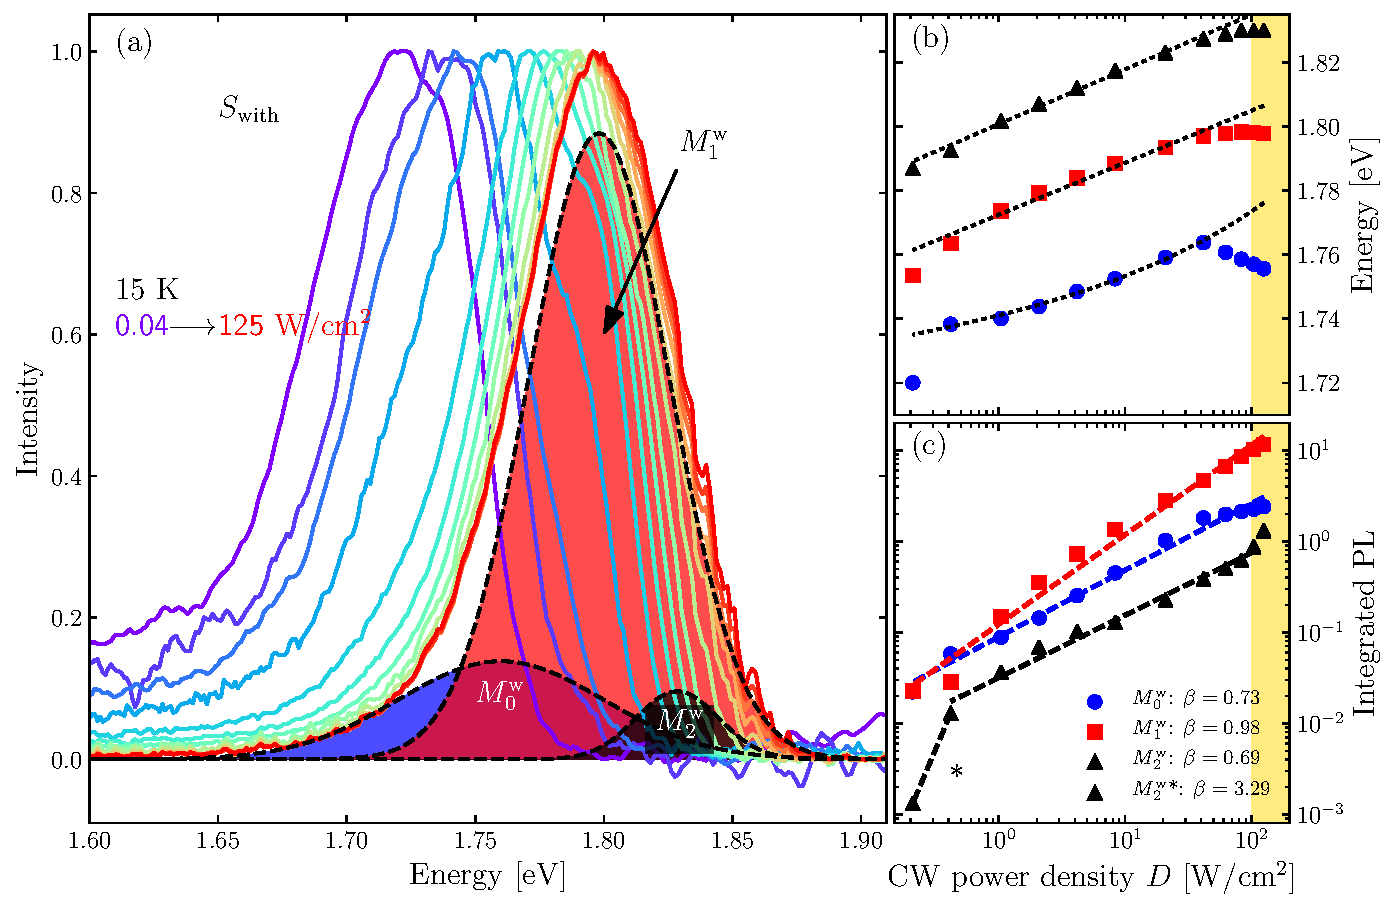
\includegraphics[width=0.9\linewidth]{/PL/intensity/12040_1113_norm_PL_int_typIvsII_saturace}
	\caption{(a) PL spectra of sample $S_\mathrm{with}$ as a function of excitation density were measured from 0.04 to 125~W/cm$^2$ and deconvolved by three Gaussian profiles: $M_0^\mathrm{w}$ (blue), $M_1^\mathrm{w}$ (red) and $M_2^\mathrm{w}$ (black shaded area). Fitted parameters, i.~e., energy and integrated PL intensity are depicted in panels (b) and (c), respectively. Energies are fitted by Eg.~\ref{eq:PL_intmodel} (dotted lines in (b)), integrated PL intensity by linear curve (dashed lines in (c)).{\color{blue}{ Symbol * labels faster increase of PL signal of band $M_2^\mathrm{w/o}$ at lower $D$. A regime of PL saturation is depicted as yellow shadowed area}}.}
	\label{fig:QD_w_int}
\end{figure}

Three Gaussian profiles ($M_0^\mathrm{w}$, $M_1^\mathrm{w}$ and $M_2^\mathrm{w}$) in PL spectra were fitted and studied as a function of excitation density $D$ in the range between 0.04 and 125~W/cm$^2$, see Fig.~\ref{fig:QD_w_int}~(a).
%
{\color{blue}{Individual bands are shifted to higher energies of 44~meV as well as the whole PL spectrum. For better insight we studied individual bends in Fig~\ref{fig:QD_w_int} where in panels (b) and (c) we show the emission energy and integrated PL intensity of individual bands as a function of $D$, respectively.}}
%
% In Fig.~\ref{fig:QD_w_int}~(b) and~(c) we show the emission energy and integrated PL intensity of individual bands as a function of $D$, respectively.
%
 Analysis of the blue-shift of individual bands distinguishes type-II aligned for $M_0^\mathrm{w}$ transition and type-I for $M_1^\mathrm{w}$ and $M_2^\mathrm{w}$. Interestingly, $M_1^\mathrm{w}$ and $M_2^\mathrm{w}$ are proportional to $\ln(D)$ via same constant ($U_\mathrm{e}+U_\mathrm{h}=7$~meV) which leads us to speculate that these transitions originate from the same structure. 
%The energies of $M_0^\mathrm{w}$ and $M_1^\mathrm{w}$ are fitted by Eq.~\ref{eq:PL_intmodel}, but we can see the third root behaviour only in the beginning of the dependence, then the energies start to be saturated. The whole evolution of energy versus pumping power is much better characterized using the self-consistent multi-particle calculations as in Ref.~\citep{Klenovsky2017}.

{\color{blue}{The dependencies for integrated PL intensity were fairly well fitted by the linear function in the whole range except of area higher than 100~W/cm$^2$ where $M_0^\mathrm{w}$ and $M_2^\mathrm{w}$ seem to be saturated.
		
The origin of $M_0^\mathrm{w}$, $M_1^\mathrm{w}$ and $M_2^\mathrm{w}$ transitions was ascertained by $\mathbf{k \cdot p}$ method as can be shown below. In this place we only designate $M_0^\mathrm{w}$ as transition in GaAs layer from electrons from $X_{xy}$ band to heavy hole state. Peaks $M_1^\mathrm{w}$ and $M_2^\mathrm{w}$ are both QD transition from $\Gamma$ and $L$ band, respectively.}}



\subsubsection*{Sample with capped QDs $\mathbf{S_\mathrm{cap}}$}
\begin{figure}
	\centering
	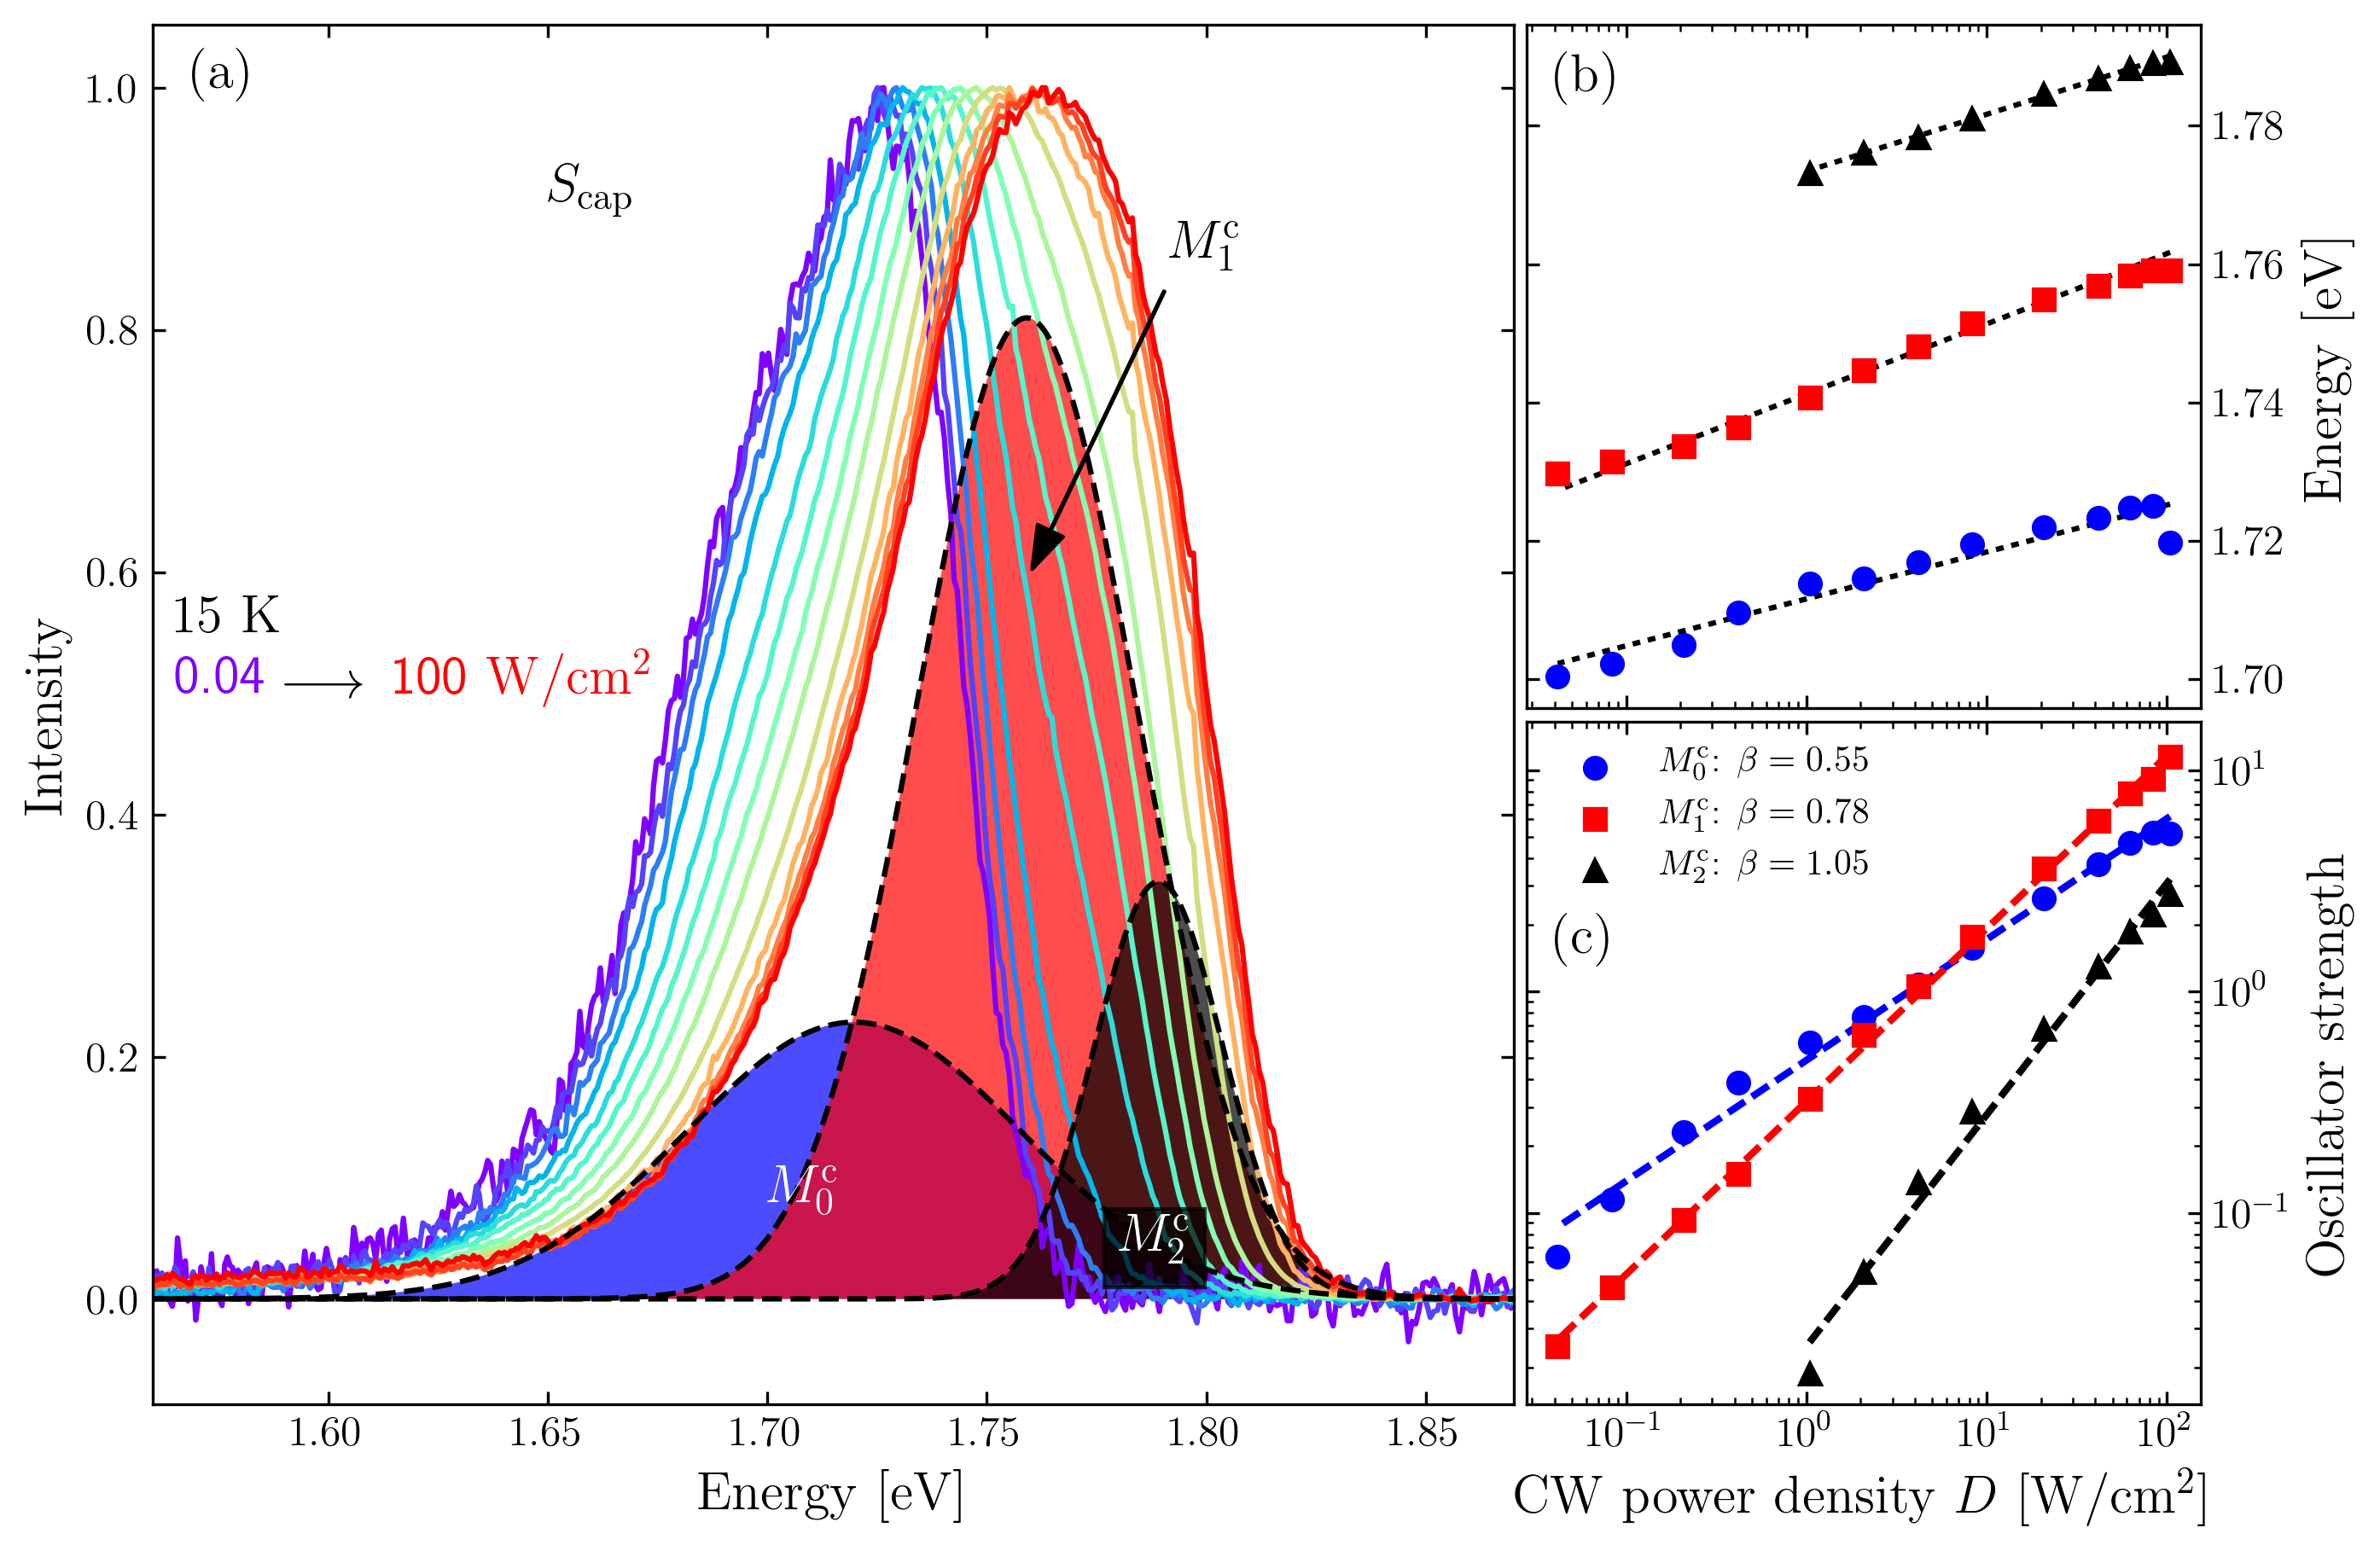
\includegraphics[width=0.9\linewidth]{/PL/intensity/12021_1108_norm_PL_int_typIvsII}
	\caption{PL spectra for sample $S_\mathrm{cap}$. The results are given in the same nomenclature as in Fig.~\ref{fig:QD_w_int}.}
	\label{fig:QD_cap_int}
\end{figure}

{\color{blue}{Intensity-resolved PL spectra of ${S_\mathrm{cap}}$ were treated similarly as for sample ${S_\mathrm{with}}$ and can be seen in Fig.~\ref{fig:QD_cap_int}. All of the bands have type-I band alignment although blue shift of whole PL spectrum of 29~meV was observed. Note, that no saturation of electronic states and no activation events occur in the measured excitation power range occur}}. All fitted parameters are summarized in Tab.~\ref{tab:int_params}.
\begin{table}
	\centering
	\caption{Summary of the fitting parameters of power density dependent PL for all samples.{\color{blue}{ Results of fit only in low excitation range are labels by symbol *.}}}
	\begin{tabularx}{1\textwidth}{cCCcc}
		\toprule
		
		transition & $E_\mathrm{I}$ [meV]&  $U_\mathrm{e}+U_\mathrm{h}$ [meV]  & $\gamma$ [$\mathrm{meV W^{-1/3}cm^{2/3}}$] & $\beta$ \\ 	
		\midrule
		\midrule
		$M_0^\mathrm{w/o}$& $1819\pm1$ & $-0.02\pm 0.06$ & $0$& $0.55\pm0.02$\\
		$M_1^\mathrm{w/o}$& $1831\pm1$ & $1.0\pm0.1$ & $0$&  $0.79\pm0.02$\\
		$M_2^\mathrm{w/o}$ & $1859\pm2$ & $1.0\pm0.2$ & $3\pm2$&  $0.66(^*1.72)\pm0.03$\\ 
		
		\midrule
		$M_0^\mathrm{w}$& $1735\pm2$ & $2\pm1$ & $6\pm2$&  $0.73\pm0.02$\\
		$M_1^\mathrm{w}$& $1772\pm4$ & $7\pm2$ & $0$&  $0.98\pm0.04$\\ %gamma=1\pm408e-5
		$M_2^\mathrm{w}$ &$1801\pm3$& $7\pm1$  &$0$ &$0.68(^*3.29)\pm0.03$\\ %gamma=0.1\pm250e-5
		
		\midrule
		$M_0^\mathrm{c}$& $1712\pm2$ &   $3\pm1$& $0$  &$0.54\pm0.02$\\ %gamm=1\pm166 e-5
		$M_1^\mathrm{c}$& $1741\pm1$ & $4.4\pm0.6$ & $0$& $0.78\pm0.01$\\ %gamma=4\pm 112 e-5
		$M_2^\mathrm{c}$ & $1773\pm3$ & $3.6\pm0.5$ & $0$&  $1.05\pm0.04$\\ %gamma=4\pm53 e-5
		
		\bottomrule
	\end{tabularx}\label{tab:int_params}
\end{table}



%\begin{table}
%	\centering
%	\caption{Summary of the fitting parameters of power density dependent PL for all samples.}
%	\begin{tabularx}{0.9\textwidth}{cCCcc}
%		\toprule
		
%		transition & $E_\mathrm{I}$ [meV]&  $U_\mathrm{e}+U_\mathrm{h}$ [meV]  & $\gamma$ [$\mathrm{meV W^{-1/3}cm^{2/3}}$] & Type \\ 	
%		\midrule
%		\midrule
%		$M_0^\mathrm{w/o}$& $1819\pm1$ & $-0.02\pm 0.06$ & $0$& Type-I\\
%		$M_1^\mathrm{w/o}$& $1831\pm1$ & $1.0\pm0.1$ & $0$& Type-I\\
%		$M_2^\mathrm{w/o}$ & $1859\pm2$ & $1.0\pm0.2$ & $3\pm2$&  Type-II\\ 
		
%		\midrule
%		$M_0^\mathrm{w}$& $1735\pm2$ & $2\pm1$ & $6\pm2$&  Type-II\\
%		$M_1^\mathrm{w}$& $1772\pm4$ & $7\pm2$ & $0$&  Type-I\\ %gamma=1\pm408e-5
%		$M_2^\mathrm{w}$ &$1801\pm3$& $7\pm1$  &$0$ &Type-I\\ %gamma=0.1\pm250e-5
%		
%		\midrule
%		$M_0^\mathrm{c}$& $1712\pm2$ &   $3\pm1$& $0$  &Type-I\\ %gamm=1\pm166 e-5
%		$M_1^\mathrm{c}$& $1741\pm1$ & $4.4\pm0.6$ & $0$& Type-I\\ %gamma=4\pm 112 e-5
%		$M_2^\mathrm{c}$ & $1773\pm3$ & $3.6\pm0.5$ & $0$&  Type-I\\ %gamma=4\pm53 e-5
		
%		\bottomrule
%	\end{tabularx}\label{tab:int_params}
%\end{table}


The evolution of the emission bands of sample $S_\mathrm{cap}$ with excitation intensity is compared with predictions obtained within the semi-self-consistent CI (SSCCI) presented in Ref.~\citep{Klenovsky2017} %and described in chapter~\ref{chap:SciRep} 
for 2.5~nm height In$_{0.15}$Ga$_{0.85}$As$_{0.85}$Sb$_{0.15}$/GaAs/GaP QD calculated by the supervisor. The band $M_1^\mathrm{c}$ is reasonably well reproduced by SSCCI with basis formed from single-particle wavefunctions calculated by $1\times8~\mathbf{k \cdot p}$ method with electrons originating from $L$ and holes form $\Gamma$-point. On the other hand, SSCCI with $8\times8~\mathbf{k \cdot p}$ basis for electrons coming from $\Gamma$-point might describe the band $M_2^\mathrm{c}$ reasonably well. {\color{blue}{Based on band edges was estimated that the third band $M_0^\mathrm{c}$ seems to be transition of electrons from $X_{xy}$-point of GaAs layer to heavy hole state of that. This statement is supported by similarity of $M_0^\mathrm{c}$ with $M_2^\mathrm{wo}$ in both $U_\mathrm{e}+U_\mathrm{h}~\sim2$~meV and $\beta$.

Similar SSCCI calculations to reproduce power evolution of bands of sample $S_\mathrm{with}$ were performed. Very well match with $M_1^\mathrm{w}$ and $M_2^\mathrm{w}$ were achieved for electrons from $\Gamma$ and $L$-band transition in QD with same dimensions but element contribution of In$_{0.25}$Ga$_{0.75}$As$_{0.95}$Sb$_{0.05}$. Interestingly, $\Gamma$ and $L$ transition swap in energy. Assign $M_0^\mathrm{w}$ to transition from $X_{xy}$ to heavy hole state in GaAs layer by comparison energy of band edges was carried out as in case of $S_\mathrm{cap}$.}}
%
\begin{figure}
	\centering
	%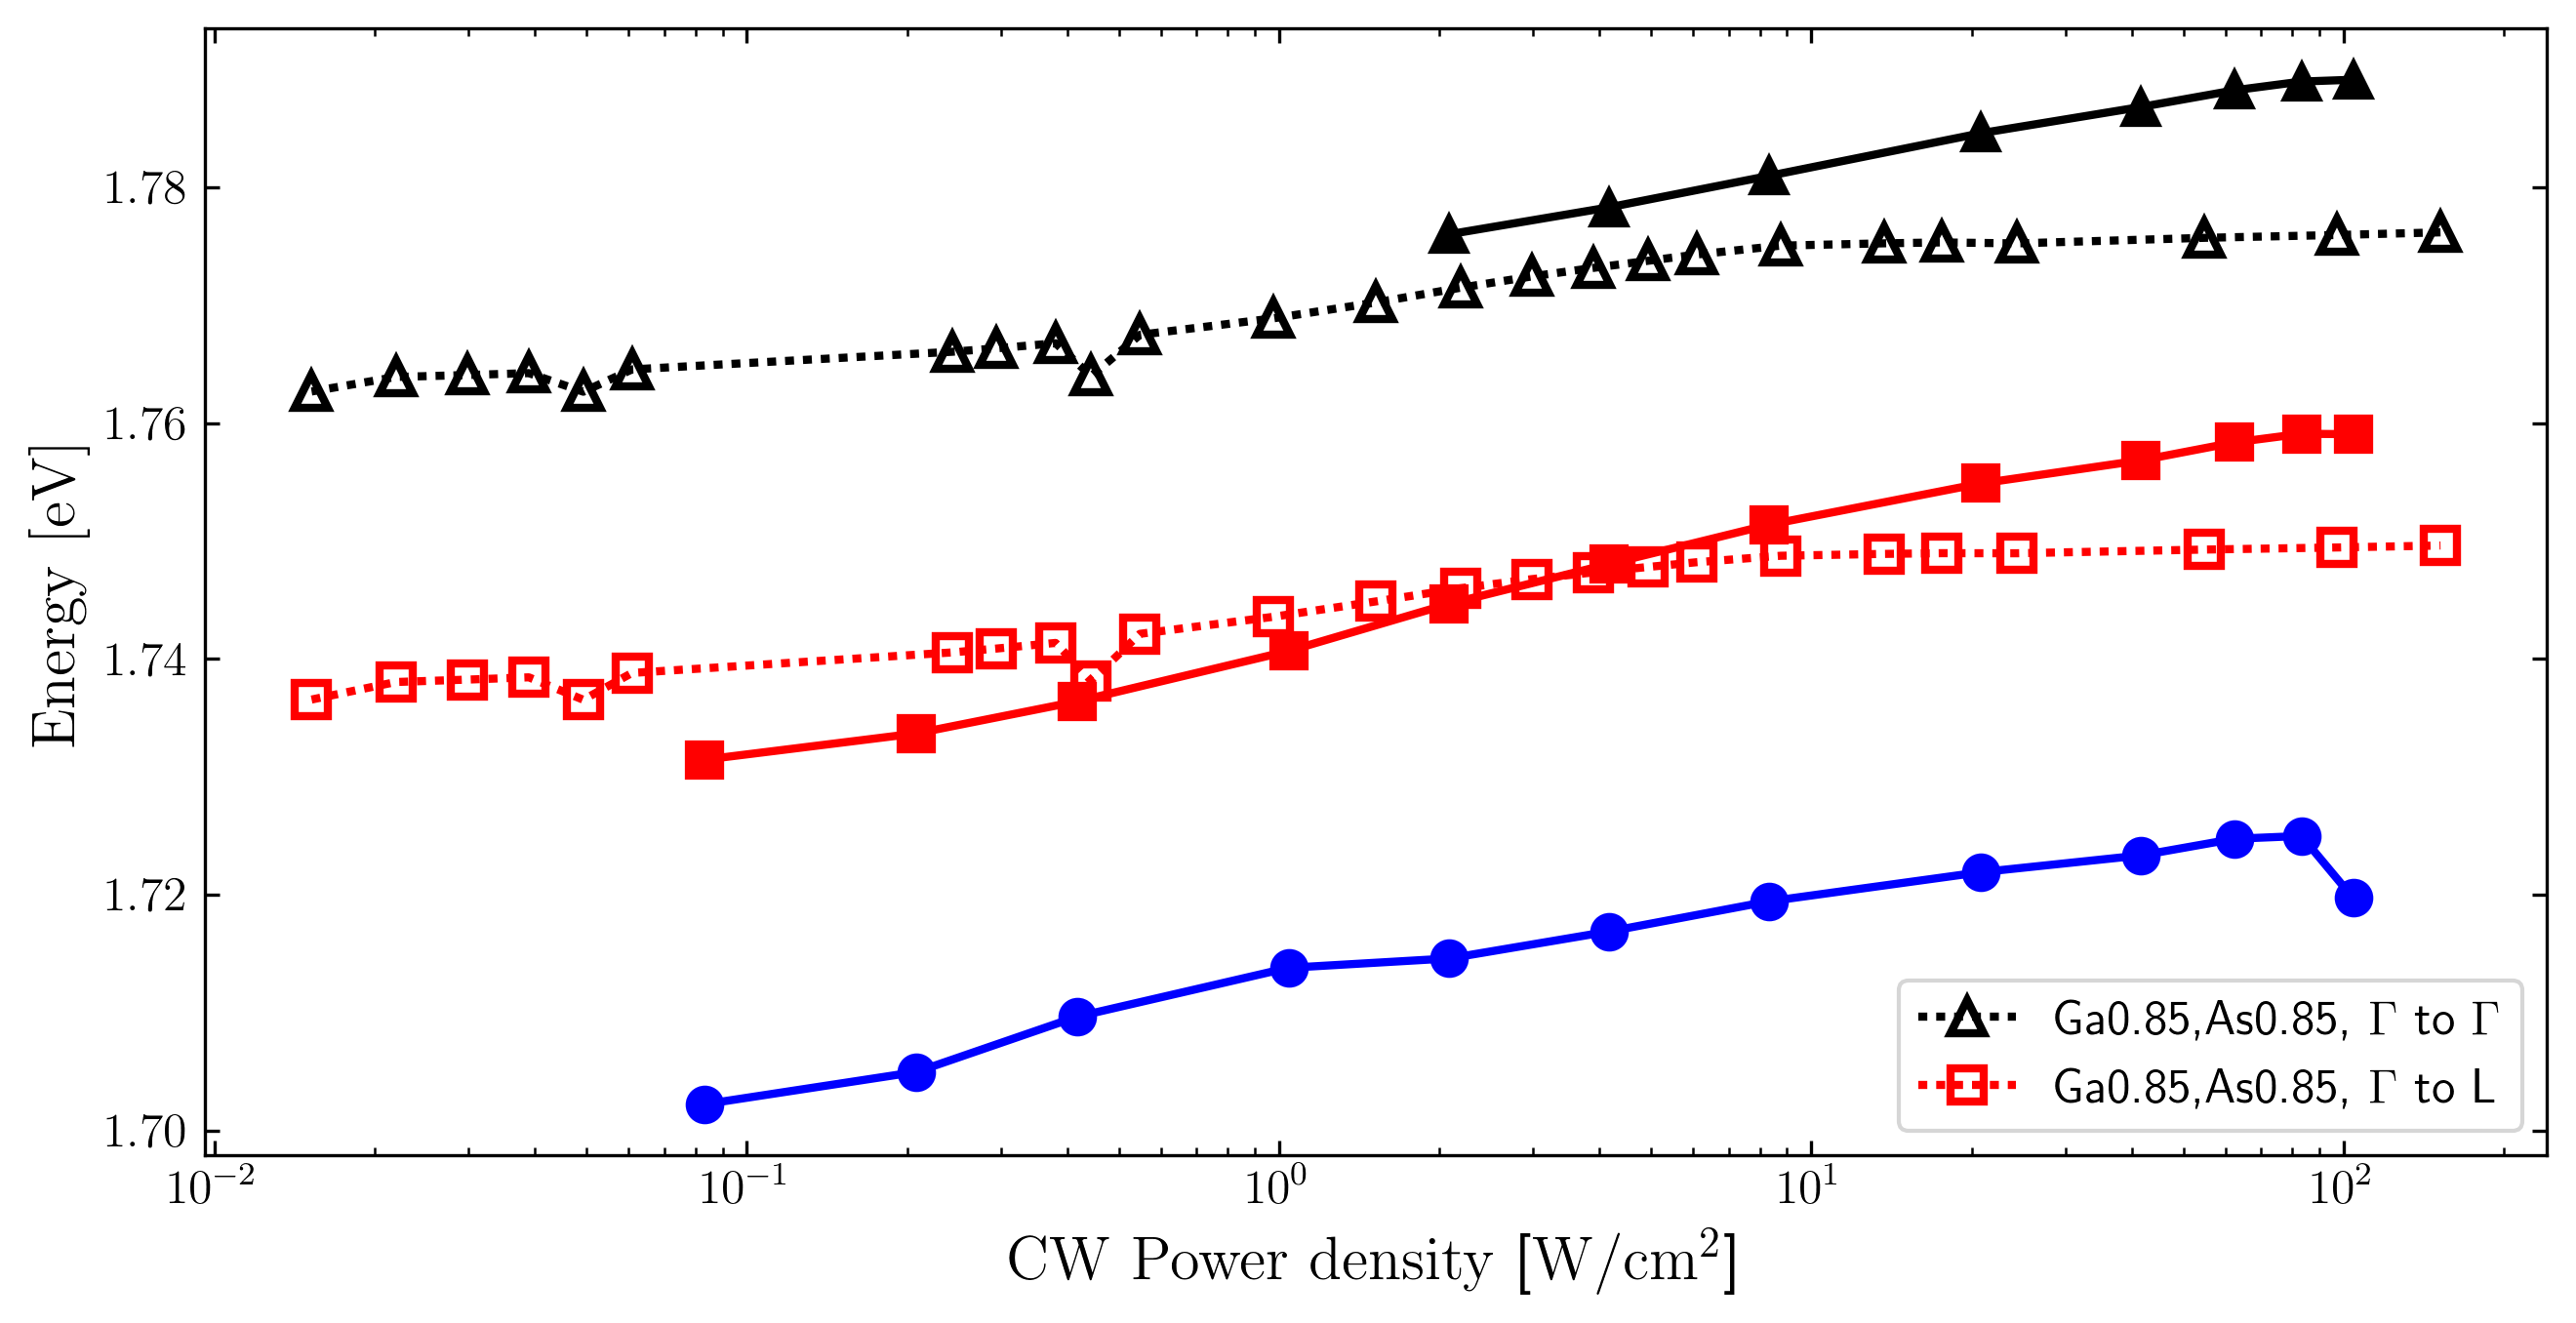
\includegraphics[width=0.9\linewidth]{/PL/intensity/12021_1107_norm_PL_int_vs_theory}
	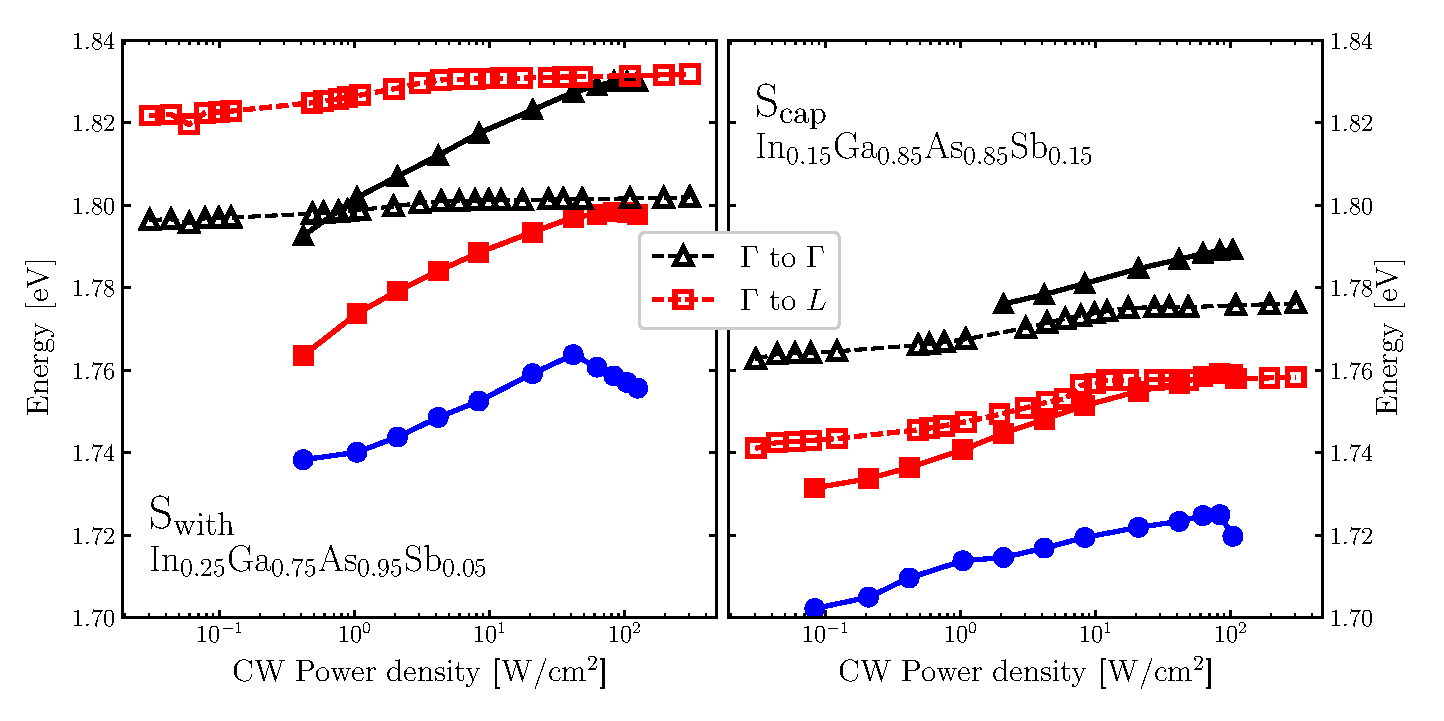
\includegraphics[width=0.9\linewidth]{/PL/intensity/QD_samples_Energy_int_vs_theory}
	\caption{Emission energy evolution with excitation intensity predicted by SSCCI with single-particle bases calculated by $1\times8~\mathbf{k \cdot p}$ and $8\times8~\mathbf{k \cdot p}$, respectively (dotted curve and open squares). To compare, experimental data are included as well~(solid curve and full squares).}
	\label{fig:QD_cap_int_expvstheory}
\end{figure}

\newpage
\subsection{Temperature dependent PL}
\label{Sec:temp_PL_TU}
PL spectra of the studied samples investigated as a function of temperature were fitted by three Gaussian profiles similarly as for the excitation density investigation in Sec.~\ref{sec:intensity_PL_TU}. The fitted energies were examined using the Varshni-like model~\cite{Taiping2014}
%
\begin{equation}
E(T)=E_0-\frac{\alpha T^2}{T+\Theta_\mathrm{D}}-\frac{\sigma^2}{k_\mathrm{B}T}, \label{eq:Varshni-like}
\end{equation}
where $E_0$ is the energy at temperature $T=0~\mathrm{K}$, $\alpha$ and $\Theta_\mathrm{D}$ are the Varshni parameters describing rate of change of the band gap with temperature and the Debye temperature corresponding with average phonon energy $\epsilon_\mathrm{D}=k_\mathrm{B}\Theta_\mathrm{D}$, respectively, $k_\mathrm{B}$ is the Boltzmann constant. The model provides the thermally dependent correction of the empirical Varshni model~\citep{Varshni} describing temperature effects on the band gap of an idealized bulk semiconductor. The estimation proposed by Eliseev~\citep{Eliseev_apl2003_PLtemp} to evaluate the correction is used, which assumes the Gaussian-type distribution of energy of the localized states with broadening parameter $\sigma$.

The mechanisms responsible for the temperature quenching of PL intensity $I_\mathrm{PL}(T)$ can be accounted for by the Boltzmann model for excitonic recombination with two characteristic activation energies~\citep{Daly_prb1995, Alen_apl2011}
\begin{equation}
I_\mathrm{PL}(T)=\frac{I_0}{1+\tau_0\left[\Gamma_1\exp(-E_1/k_\mathrm{B}T)+\Gamma_2\exp(-E_2/k_\mathrm{B}T)\right]},               \label{eq:Arhenius}
\end{equation}
where $I_0$ is the intensity at 15~K (lowest temperature reached in our measurements), $\tau_0$ temperature-independent radiative recombination time at 15~K, $E_1$ and $E_2$ are the activation energies of the two quenching mechanisms with related scattering rates $\Gamma_1$ and $\Gamma_2$.%These parameters are representative of the average behaviour of the emissions bands, being the most important $\tau_0$, $E_1$ and $E_2$.
\newpage
\subsubsection*{Sample without QDs $\mathbf{S_\mathrm{w/o}}$}
%
Three recognized emission bands ($M_0^\mathrm{w/o}$, $M_1^\mathrm{w/o}$, and $M_2^\mathrm{w/o}$) in PL of sample ${S_\mathrm{w/o}}$ are individually investigated for temperatures from 15~K to 130~K, see Fig.~\ref{fig:QD_wo_temp}~(a). The bands are  Varshni-like energy-shifted,
% described by parameters
% listed in Tab.~\ref{tab:Varshni}, 
see Fig.~\ref{fig:QD_wo_temp}~(b). Interestingly, the bands $M_1^\mathrm{w/o}$ and $M_2^\mathrm{w/o}$ representing phonon and no-phonon assisted $X_{xy}$ to heavy hole transition share temperature evolution, where $\alpha$ of $2.1\cdot10^{-4}~\mathrm{eVK^{-1}}$ is half to the value for unstrained GaAs~\cite{ioffe, Vurgaftman}. The Debye temperature $\Theta_\mathrm{D}~\sim70$~K is also significantly smaller value usually refer in literature.

In Fig.~\ref{fig:QD_wo_temp}~(c) intensity quenching through the temperature range evaluated by the Boltzmann model~(\ref{eq:Arhenius}) is shown. The value of $E_1$ (8--12~meV) corresponding to Eq.~(\ref{eq:Arhenius}) is comparable for every fitted PL band and it present also in other samples. This low activation energy is determining the low-temperature quenching of the PL and it is usually associated to carrier recombination trough impurities~\cite{YuCardona}. Most probably the quenching mechanism is related to nitrogen complexes with activation energy $E_\mathrm{A}=8$~meV~\cite{ioffe} which is often present in GaP growth~\cite{Skazochkin_GaPtraps}. Energies label $E_2$ are activation energies of escape electrons from $X_{xy}$ band to GaP matrix ($E_2=59$~meV) or activation phonon $E_2=29$~meV in phonon replica band $M_1^\mathrm{w/o}$. 
%
\begin{figure}
	\centering
	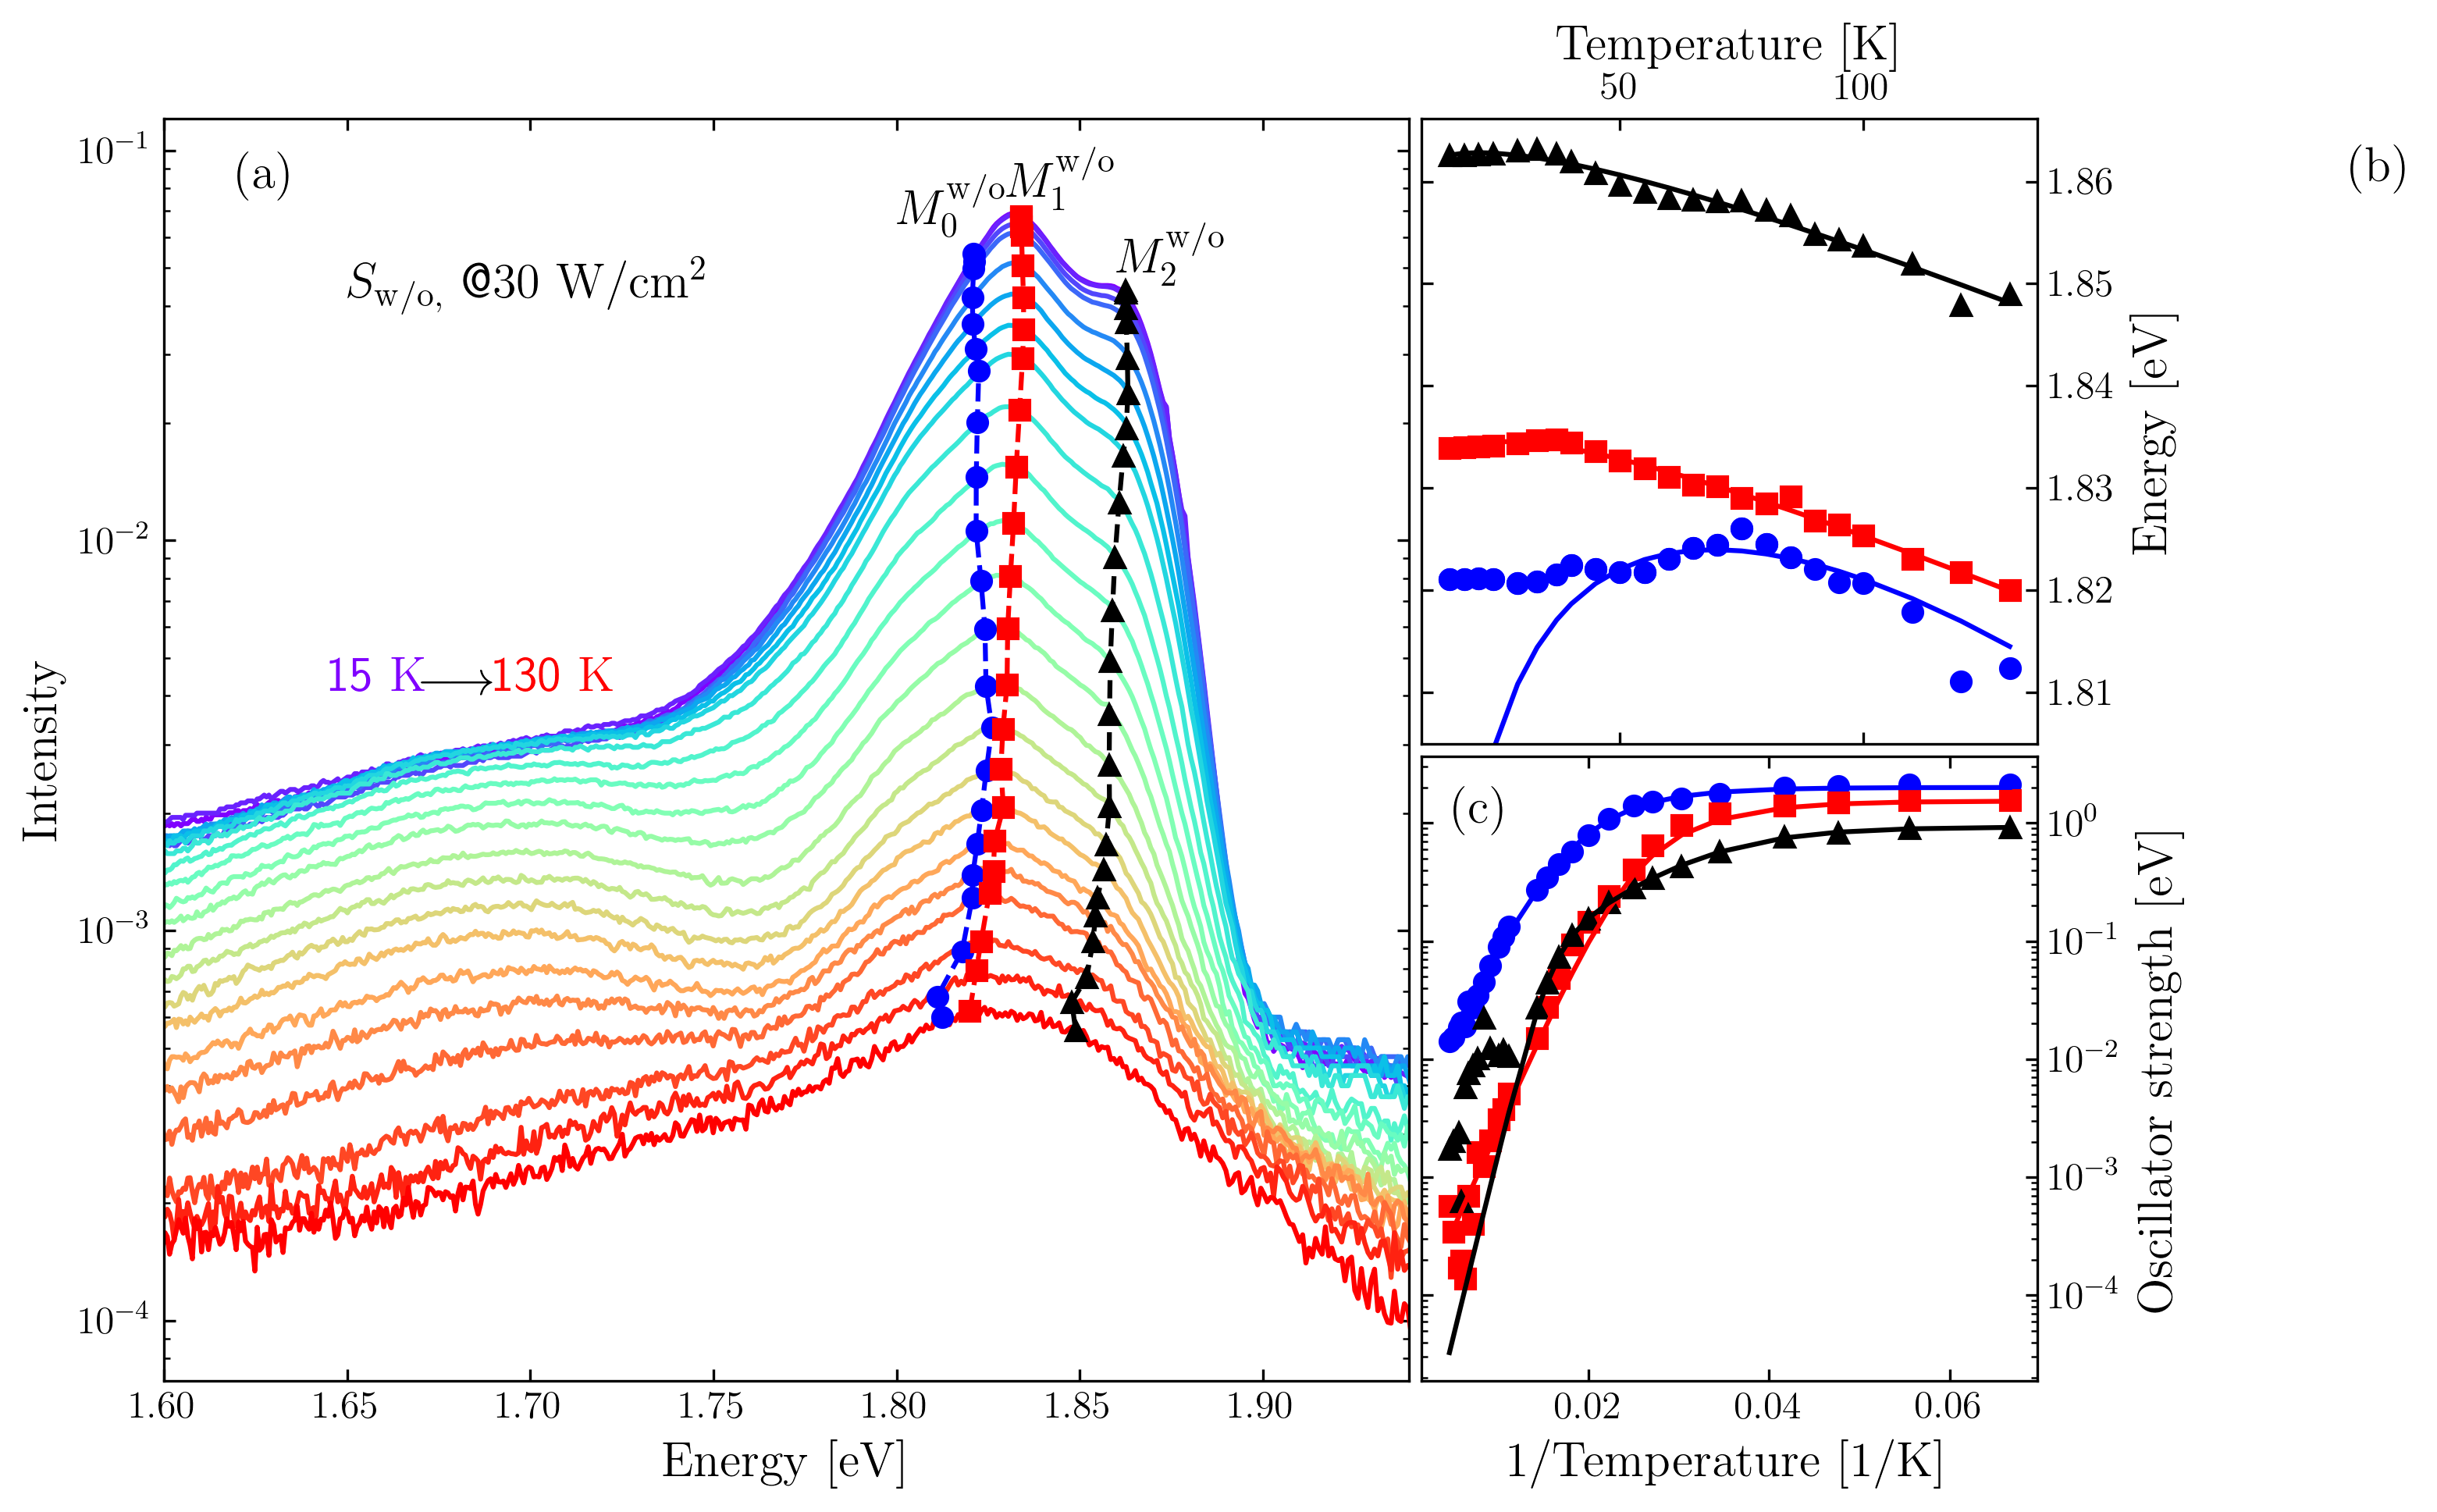
\includegraphics[width=0.9\linewidth]{/PL/temperature/12027_7mW_log_PL_int_without}
	\caption{(a) PL spectra of sample $S_\mathrm{w/o}$ measured with excitation density of 30~W/cm$^2$ in 15-130~K temperature range. Each spectrum is fitted by a sum of three Gaussian profiles represented by symbols in panel (a): $M_0^\mathrm{w/o}$ blue circles, $M_1^\mathrm{w/o}$ red squares and $M_2^\mathrm{w/o}$ black triangles. The bands are similarly marked in panels (b) and (c) where also the experimental transition energies (symbols) and fits by the Varshni model~(\ref{eq:Varshni-like}) (lines), respectively, and the integrated PL intensity (symbols) fitted by the Boltzmann model~Eq.~(\ref{eq:Arhenius}) are presented. All fitting parameters are listed in Tabs.~\ref{tab:Varshni} and~\ref{tab:Arhenius}.}
	\label{fig:QD_wo_temp}
\end{figure}


\subsubsection*{Sample with QDs $\mathbf{S_\mathrm{with}}$}
%
For sample $S_\mathrm{with}$ in temperature range between 15 and 150~K we observe quenching of PL intensity of three optical transitions marked $M_0^\mathrm{w}$, $M_1^\mathrm{w}$ and $M_2^\mathrm{w}$, see Fig.~\ref{fig:QD_w_temp}~(a). The transition energies [Fig.~\ref{fig:QD_w_temp}~(b)] and the integrated PL intensity [Fig.~\ref{fig:QD_w_temp}~(c)] are again fitted by the Varshni model~Eq.~(\ref{eq:Varshni-like}) and the Boltzmann model~Eq.~(\ref{eq:Arhenius}), respectively. % , in the whole measured temperature range.  
%
From an analysis of energy peaks shifts of $M_1^\mathrm{w}$ and $M_2^\mathrm{w}$ bands were found $\alpha$ very similar to GaAs and GaSb literature values~\cite{Vurgaftman}. From this similarity, we assume that the bands originate from structures with a high amount of Ga which is in agreement with results obtained on these structures by EDX. The decrease of $\Theta_\mathrm{D}$ in comparison to bulk values listed in Tab.~\ref{tab:Varshni} is probably related to quantum confinement of the structures.

Arrhenius plot, as in the case of sample $S_\mathrm{w/o}$, points to low-temperature quenching with activation energy around 10~meV which probably originating from nitrogen traps as it was dissuaded above. Moreover, escape energies of electrons from QDs of 197~meV and 108~meV for $\Gamma$ and $L$ band were determined. 
%
\begin{figure}
	\centering
	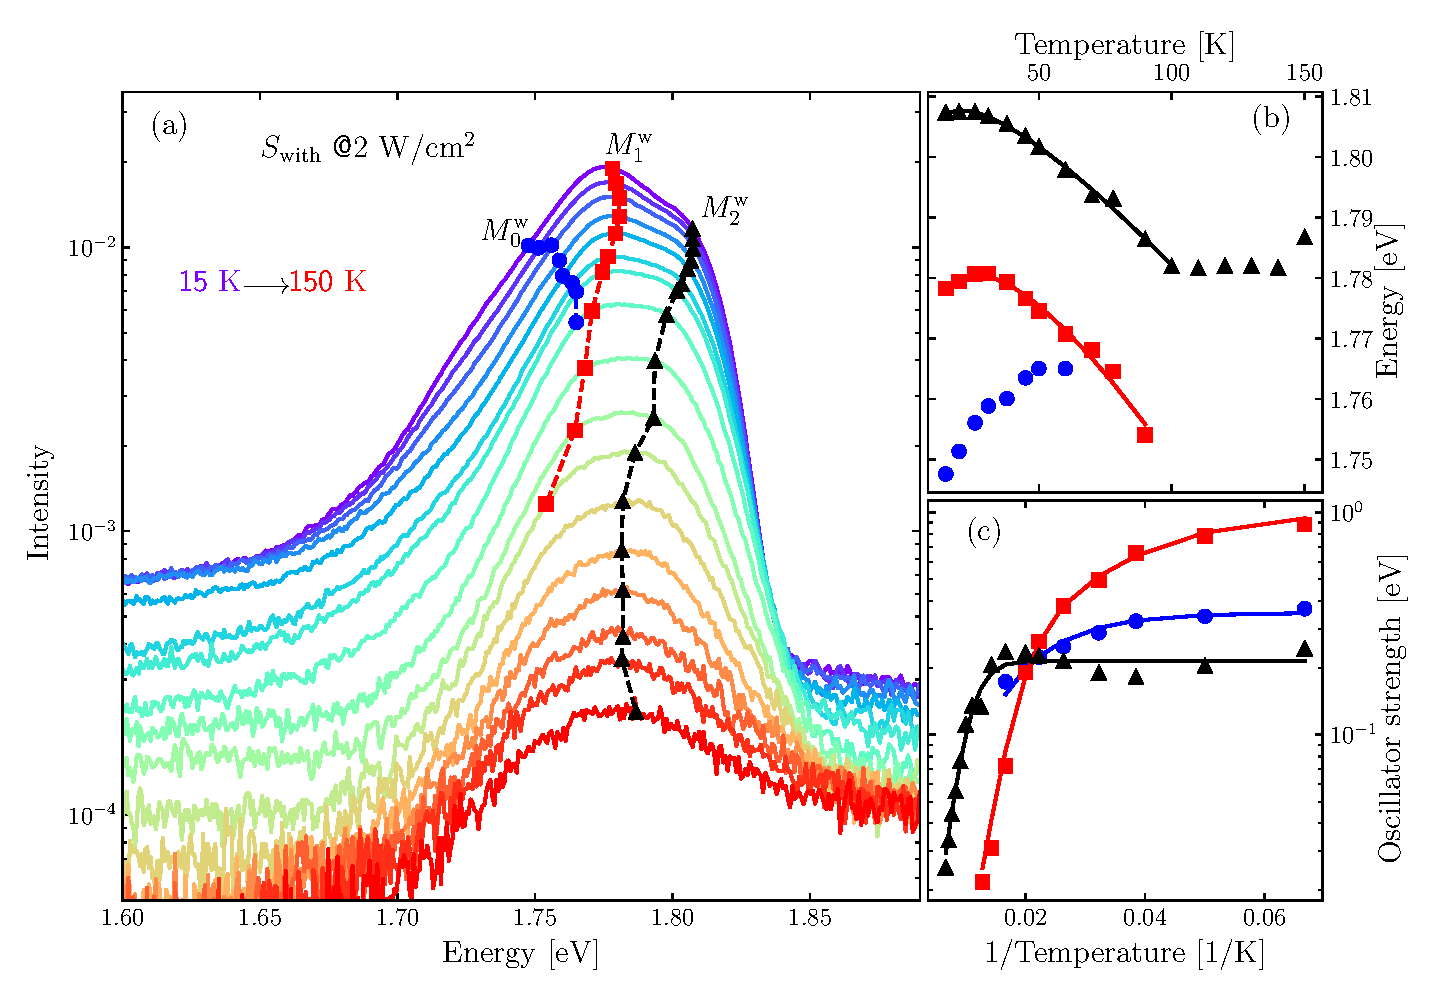
\includegraphics[width=0.9\linewidth]{/PL/temperature/12040_500uW_log_PL_int_Varshni}
	\caption{PL spectra of the sample ${S_\mathrm{with}}$ at 2~W/cm$^2$ between 15 and 150~K. The results are given in the same way as in Fig.~\ref{fig:QD_wo_temp}.}
	\label{fig:QD_w_temp}
\end{figure}

%\newpage
\subsubsection*{Sample with capped QDs $\mathbf{S_\mathrm{cap}}$}
%
PL spectra of sample ${S_\mathrm{cap}}$ are again fitted by three bands ($M_0^\mathrm{c}$, $M_1^\mathrm{c}$, and $M_2^\mathrm{c}$) and investigated in temperature range 15--110~K, see Fig.~\ref{fig:QD_c_temp}.

Looking at the parameters obtained by Varshni fit of individual bands, it seems that temperature evolution of PL describing by $\alpha$ parameter from sample ${S_\mathrm{cap}}$ is almost similar like that for ${S_\mathrm{with}}$, i.~e., between bulk values of GaAs and GaSb, which can again point to high amount of Ga in ${S_\mathrm{cap}}$. On the other hand, the Debay temperatures $\Theta_\mathrm{D}$ are larger than that on ${S_\mathrm{with}}$, but they are closer to bulk values of GaAs or GaSb, see Tab.~\ref{tab:Varshni}. These results are not surprise because growth of identical QDs following by GaSb capping layer was expected.

From the Arhenius plot of individual bands and their fits by Eq.~(\ref{eq:Arhenius}) were determined two or three, in case $M_0^\mathrm{c}$ band, temperature quenching processes. The low-temperature one characterized by activation energy $E_1\sim 10$~meV is similar like in case of previous samples and was discussed above. The higher temperature quenching processes have energy comparable with energies nesecary to escape electron from the structure (electron in localized in GaAs layer in $X_{xy}$ and $\Gamma$ to GaP matrix: $E_2=33$~meV and $E_2=519$~meV; electron in QD from $L$ and $\Gamma$ to GaP matrix: $E_2=65$~meV and $E_2=179$~meV.)

%
\begin{figure}[h]
	\centering
	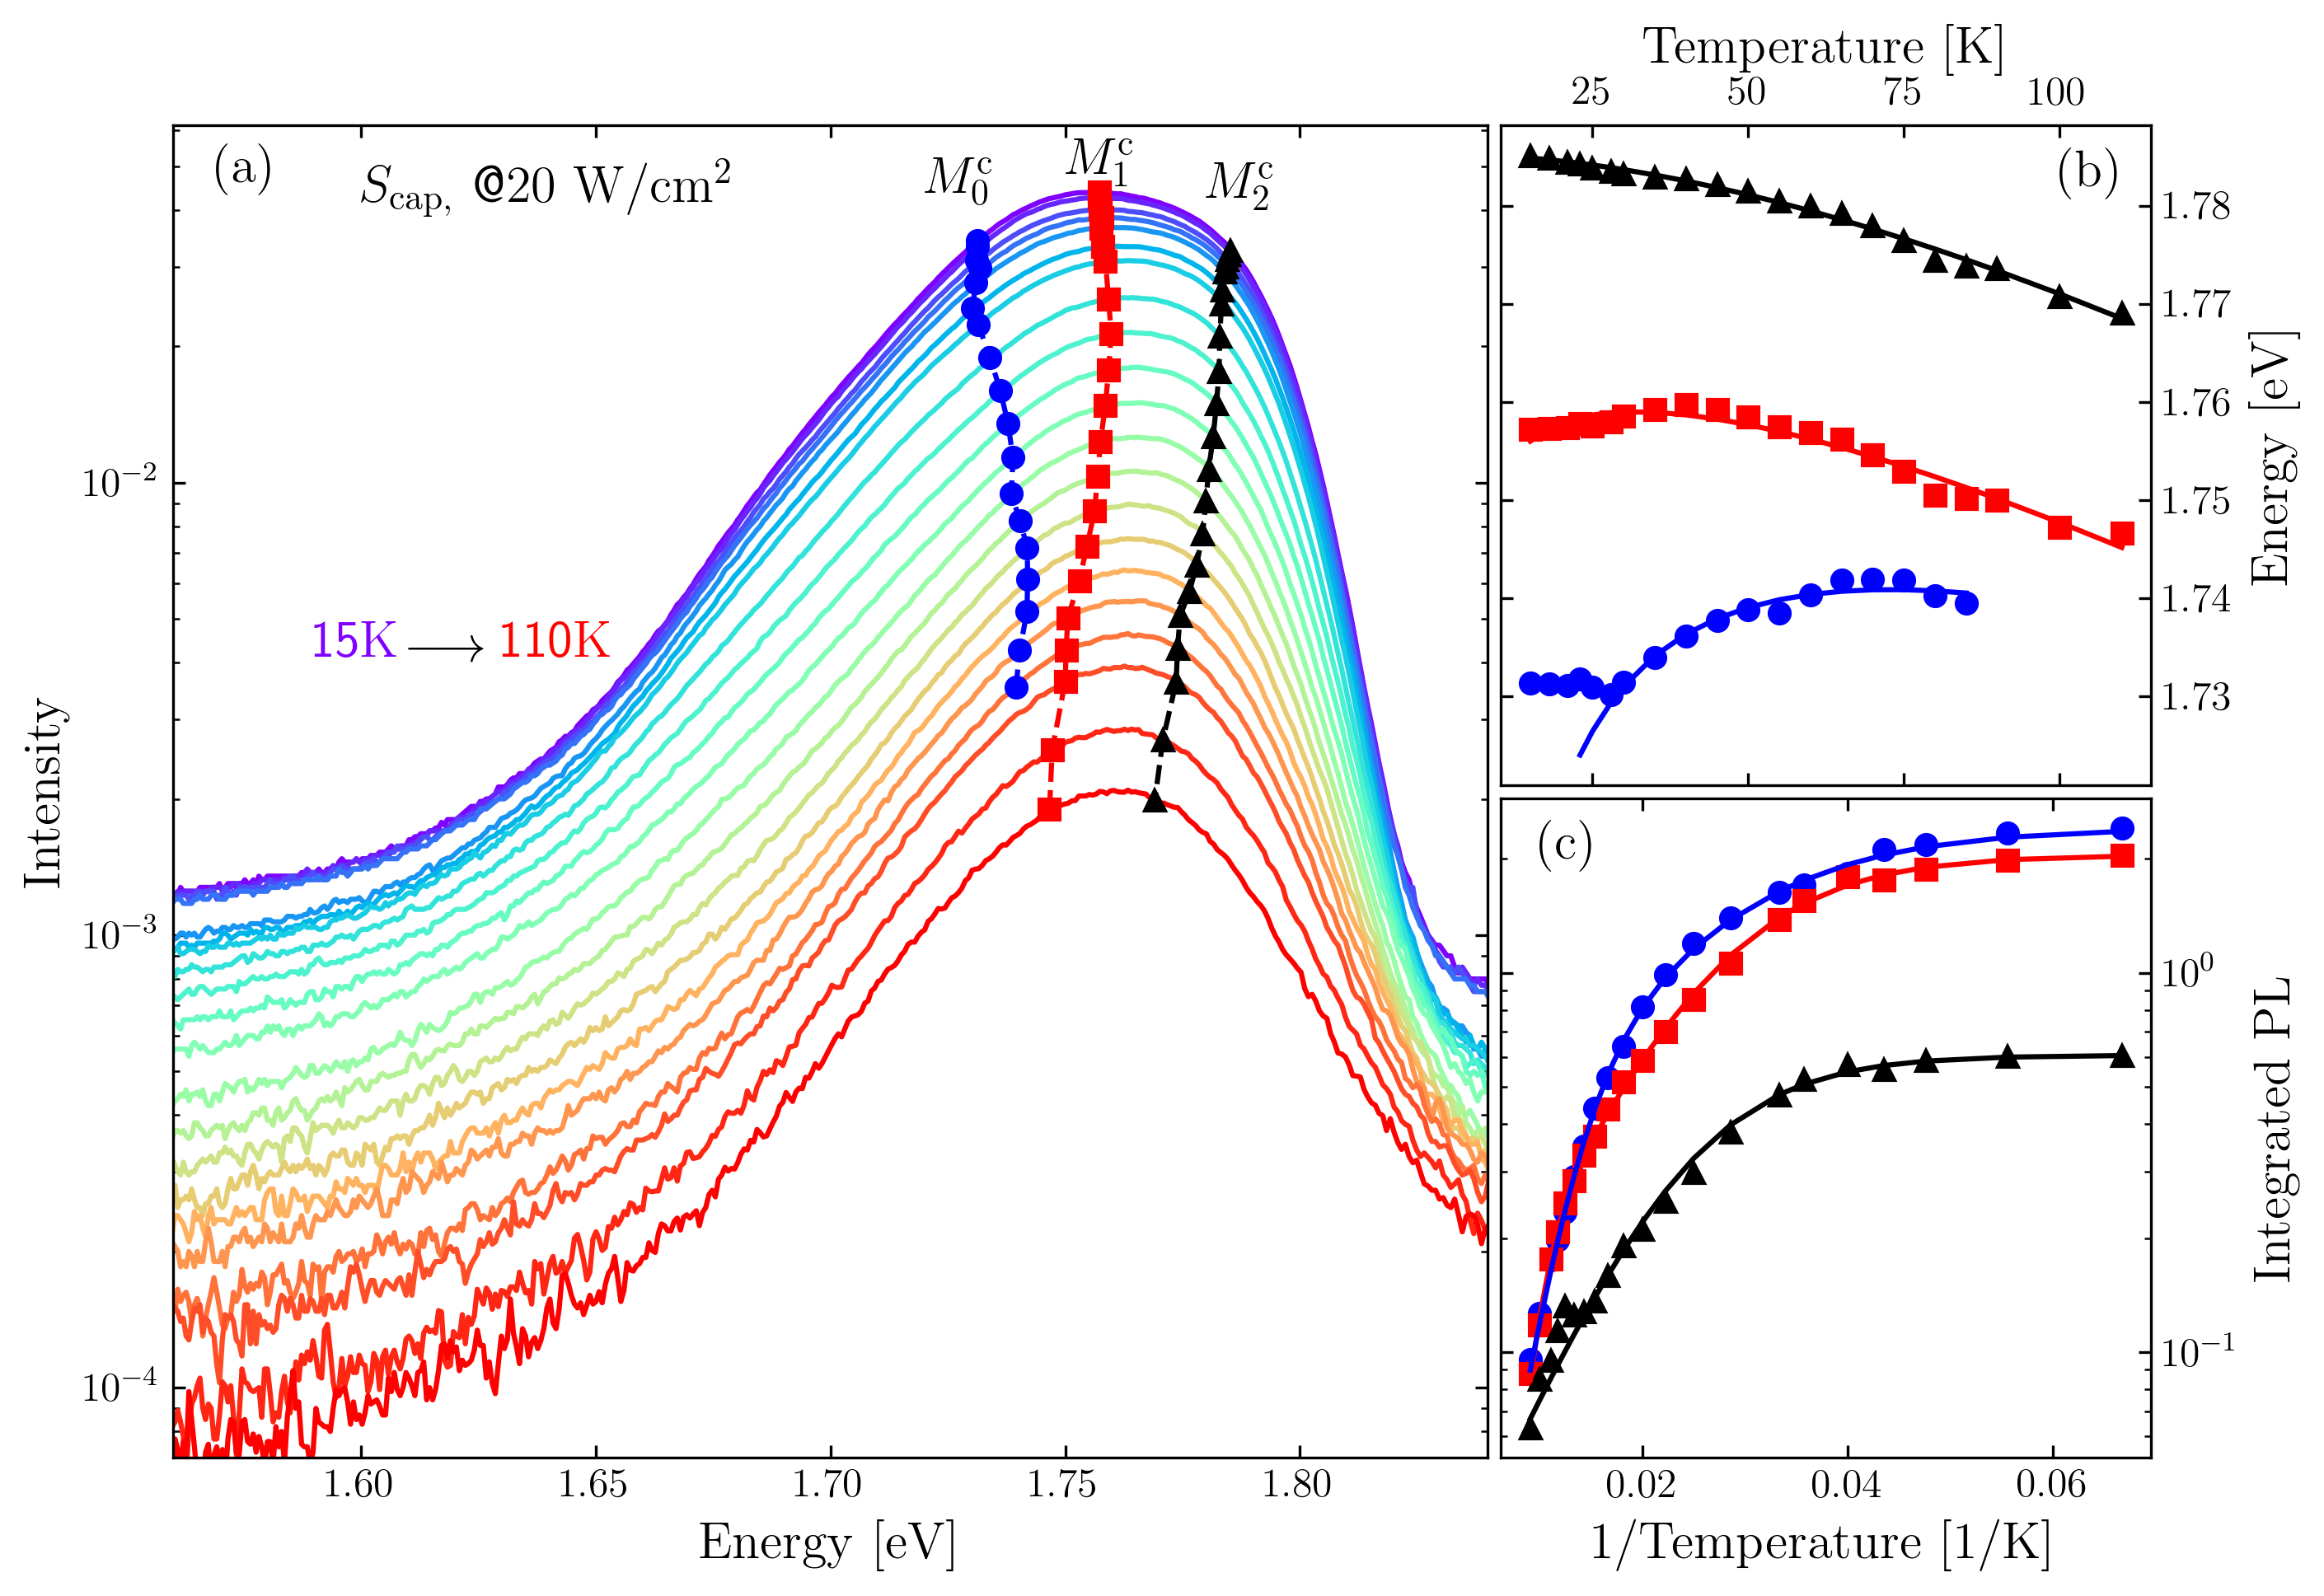
\includegraphics[width=0.9\linewidth]{/PL/temperature/12021_5mW_log_PL_int_Varshni}
	\caption{PL spectra of sample ${S_\mathrm{cap}}$ measured at 20~W/cm$^2$ between 15 and 110~K. The results are given in the same nomenclature as in Fig.~\ref{fig:QD_wo_temp}.}
	\label{fig:QD_c_temp}
\end{figure}

%\newpage

%
%The value of $E_1$ (4--15~meV) corresponding to Eq.~(\ref{eq:Arhenius}) is comparable for all samples and also for every fitted PL band. This low activation energy is determining the low-temperature quenching of the PL and it is usually associated to carrier recombination through impurities~\cite{YuCardona}. The values of the high-temperature quenching $E_2$ (29--43~meV) are also similar across the samples except the deviation in $M_2^\mathrm{c}$ where we measured extremely small activation energy ($E_2=1$~meV) and $M_2^\mathrm{w/o}$ with $E_2$ twice larger than for other bands ($E_2=62$~meV), see Fig.~\ref{fig:Arrhenius_all}.



Finally, for a summary of identified parameters for our samples by models~(\ref{eq:Varshni-like}) and~(\ref{eq:Arhenius}) which was discussed above see Tabs.~\ref{tab:Varshni} and~\ref{tab:Arhenius}, respectively. 

The obtained activation energies of escape processes will be used in Sec.~\ref{sec:TUB_results} where all experimental results will be summarized.


%\begin{figure}
%	\centering
%	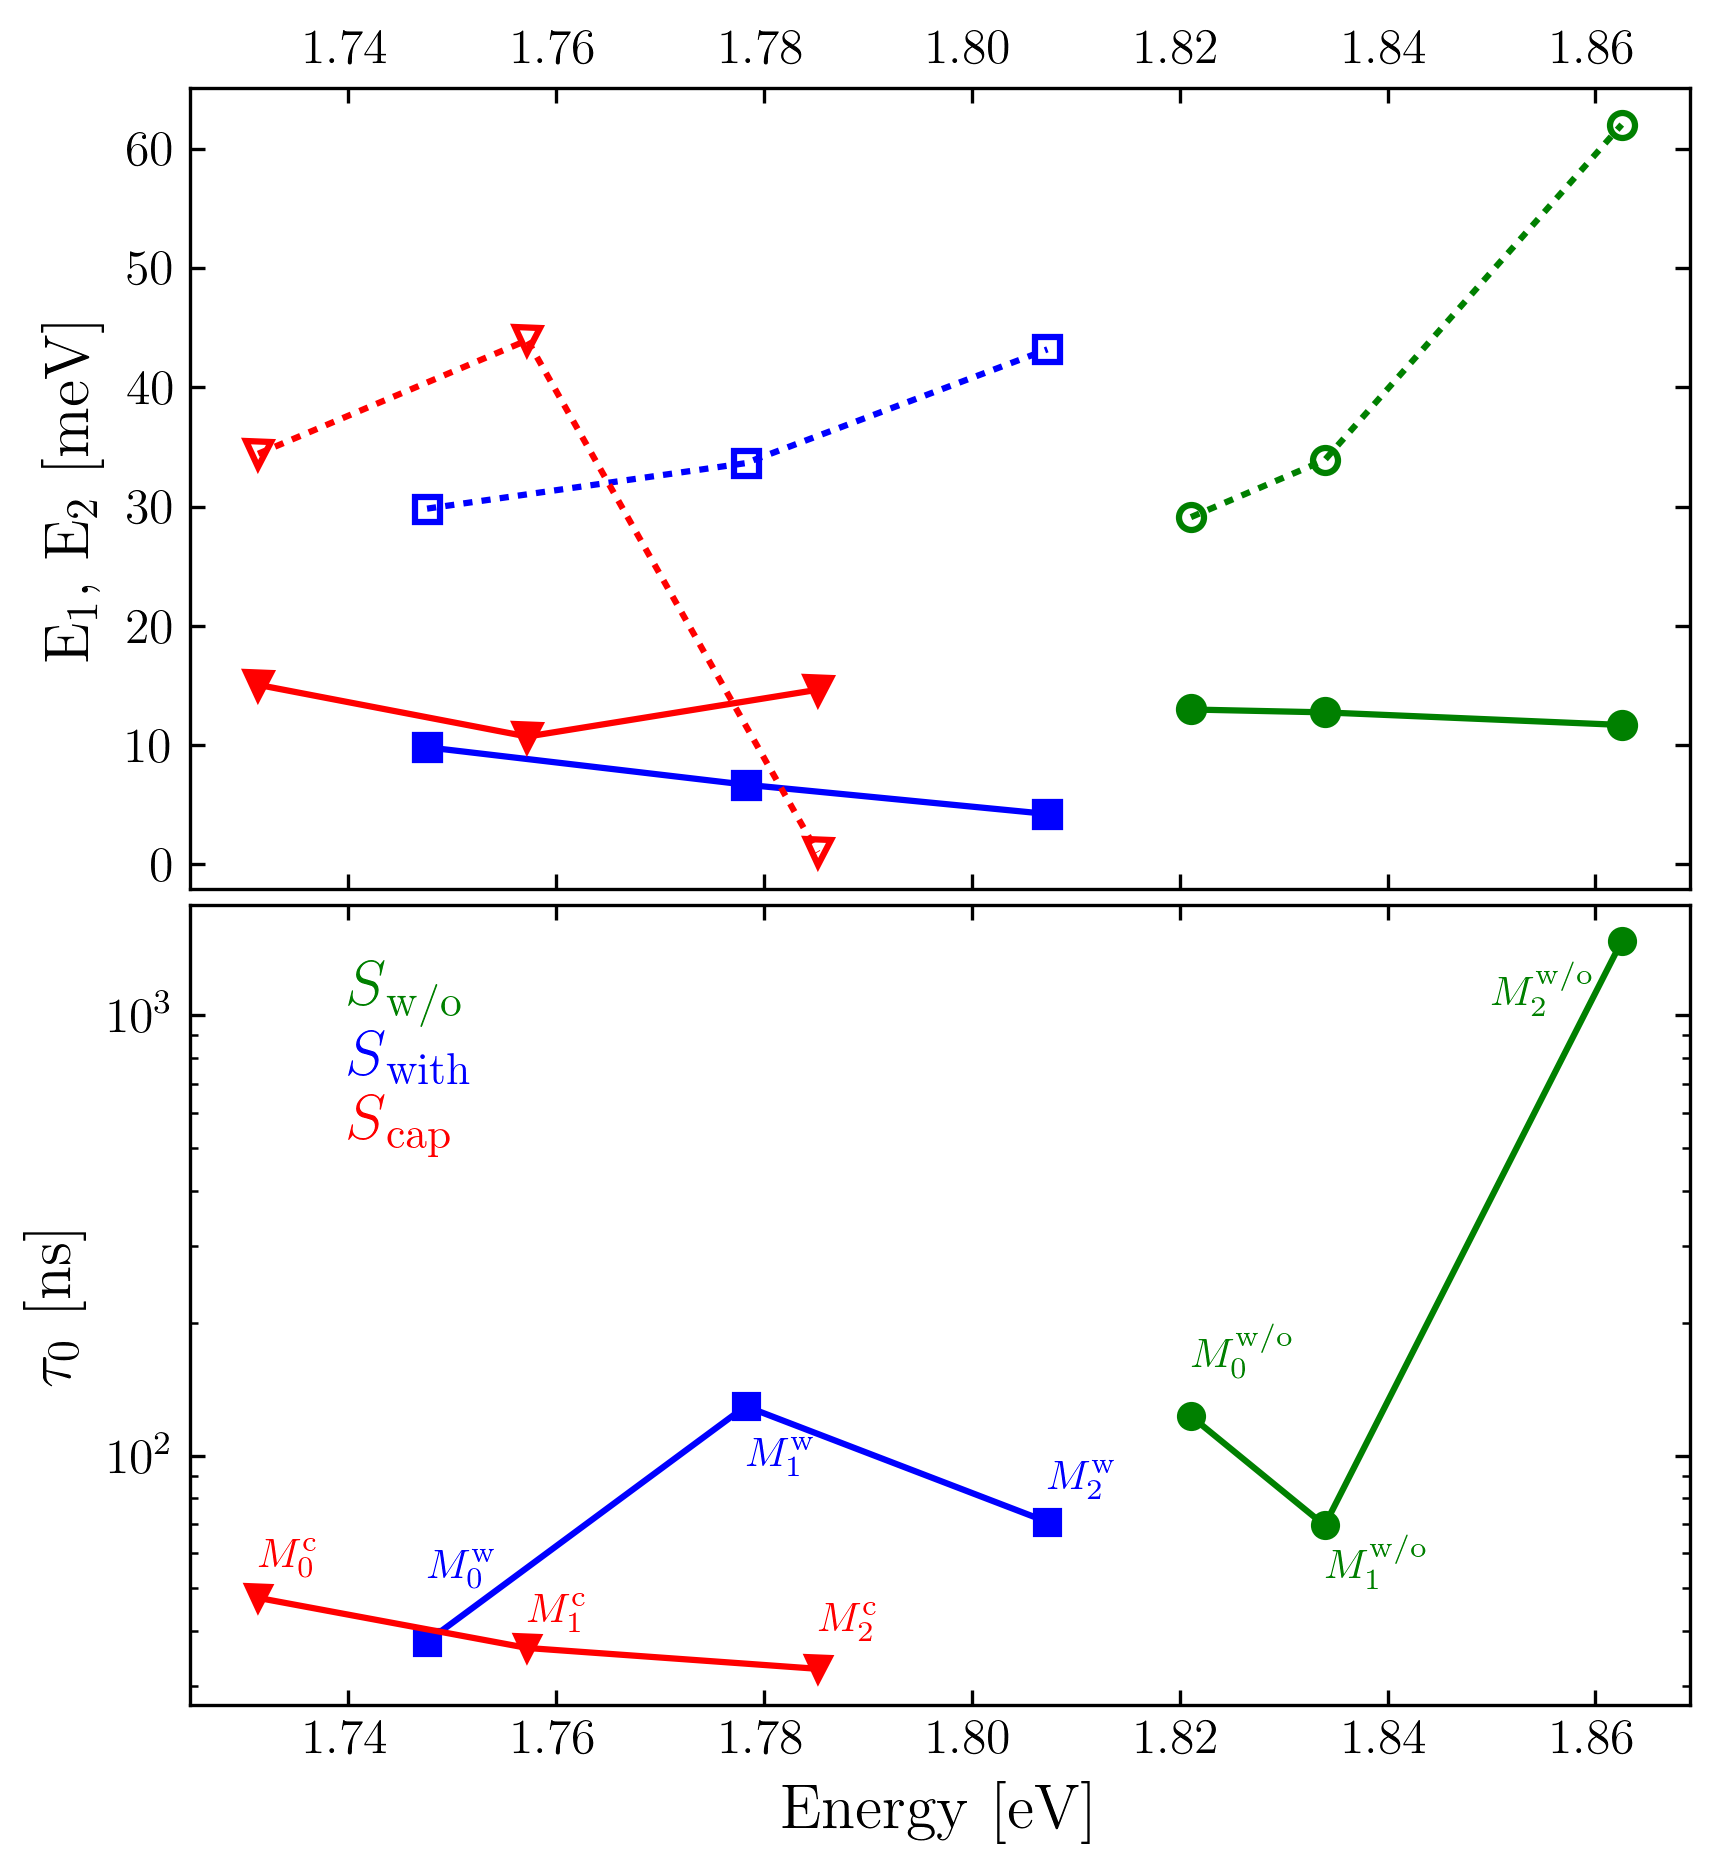
\includegraphics[width=0.75\linewidth]{/PL/temperature/all_Arhenius}
%	\caption{Comparison of the Boltzmann fitting parameters for the studied samples. The upper panel depicts $E_1$ (empty symbols) and $E_2$ (full symbols), respectively, the bottom panel shows $\tau_0$. Samples are distinguished by the type and colour of symbols as in Fig.~\ref{fig:PL_homogenity}.}
%	\label{fig:Arrhenius_all}
%\end{figure}


\begin{table}
	\centering
	\caption{Summary of the Varshni-like fits. The accuracy of $E_0$ and $\alpha$ are better than $10^{-4}\%$, and better than 5~\% for $\Theta_\mathrm{D}$ and $\sigma$. For comparison bulk values of expected materials taken from Ref.~\cite{Vurgaftman} are added. The avarage phonon energies $\epsilon_\mathrm{D}=k_\mathrm{B}\Theta_\mathrm{D}$.}
	\begin{tabularx}{1\textwidth}{cccccc}
		\toprule
		
		%transition & $E_0$ [meV]& $\alpha$ [$10^{-4}~\mathrm{eVK^{-1}}$]& $\Theta_\mathrm{D}$ [K]& $\sigma$ [meV]\\ 	
		transition & $E_0$ [meV]& $\alpha$ [$10^{-4}~\mathrm{eVK^{-1}}$]& $\Theta_\mathrm{D}$ [K]& $\sigma$ [meV]&  $\epsilon_\mathrm{D}$ [meV]\\ 	
		\midrule
		\midrule
		$M_0^\mathrm{w/o}$& $1845$ & $7.99$& $450$&$9.1$& 38.8\\
		$M_1^\mathrm{w/o}$& $1838$ & $2.14$& $67$&$2.4$&5.8\\
		$M_2^\mathrm{w/o}$ & $1865$ & $2.10$& $78$& $1.7$&6.7\\ 
		
		
		%$M_0^\mathrm{w/o}$& $1845$ & $7.99$& $450$&$9.1$\\
		%$M_1^\mathrm{w/o}$& $1838$ & $2.14$& $67$&$2.4$\\
		%$M_2^\mathrm{w/o}$ & $1865$ & $2.10$& $78$& $1.7$\\ 
		
		\midrule
		$M_0^\mathrm{w}$& $1829$ & $10.00$& $55.3$& $13.2$&4.6\\
		$M_1^\mathrm{w}$& $1798$ & $4.54$& $11.7$&$4.6$&1.0\\
		$M_2^\mathrm{w}$ & $1815$& $4.78$& $48.8$& $3.0$&4.2\\ 
		
		
		
		%$M_0^\mathrm{w}$& $1789$ & $10.00$& $270$& $8.1$\\
		%$M_1^\mathrm{w}$& $1789$ & $23.37$& $150.1$&$3.6$\\
		%$M_2^\mathrm{w}$ & $1815$& $5.49$& $74.5$& $2.8$\\ 
		
		\midrule
		%$M_0^\mathrm{c}$& $1756$ & $5.00$& $420$& $7.9$\\
		%$M_1^\mathrm{c}$& $1766$ & $4.03$& $144.5$& $3.4$\\
		%$M_2^\mathrm{c}$ & $1785$ & $4.90$& $243.2$& $1.7\cdot 10^{-5}\pm0.06$\\%$3.3\cdot 10^{-7}$\\
		
		
		$M_0^\mathrm{c}$& $1756$ & $5.00$& $420$& $7.9$&36.2\\
		$M_1^\mathrm{c}$& $1766$ & $4.03$& $144.5$& $3.4$&12.5\\
		$M_2^\mathrm{c}$ & $1785$ & $4.90$& $243.2$& $2\cdot 10^{-5}\pm0.1$&21.0\\%$3.3\cdot 10^{-7}$\\
		\midrule
		GaAs, $\Gamma$ ($X$)& 1981 (1519)& 4.60 (5.405)& 204& -&17.6\\
		GaSb, $\Gamma$ ($L$)& 812 (875)& 4.17 (5.97)& 140& -&12.1\\
		InAs, $\Gamma$ ($L$)& 417 (1133)& 2.76& 93& -&8.0\\
		InSb, $\Gamma$ ($L$)& 235 (930)& 3.20& 170& -&14.7\\
		GaP, $\Gamma$ ($L$)& 2886 (2720)& 5.77& 372& -&32.1\\
		%GaP, $L$& 2720& 5.77& 372& -&106.0&32.1\\
		\bottomrule
	\end{tabularx}\label{tab:Varshni}
\end{table}

\begin{table}
	\centering
	\caption{Summary of the Arhenius-like fits. The displayed values are obtained with accuracy better than $10^{-4}~\%$. Scattering rates $\Gamma_i$ are present as non-radiative times $\tau_i^\mathrm{NR}=1/\Gamma_i$. Units of presented quantities: $E$ [meV], $\tau^\mathrm{NR}$ [ns].}
	\begin{tabularx}{1\textwidth}{cCCCCCCCCC}%{cCCccccccc}
		\toprule
		
		%transition & $I_0$ & $\tau_0$ [ns]& $\Gamma_1$ [ns$^{-1}$]& $E_1$ [meV]& $\Gamma_2$ [ns$^{-1}$]& $E_2$ [meV]\\ 	
	%	\midrule
	%	\midrule
	%	$M_0^\mathrm{w/o}$& 7.65135744e-01&   65.2916823&   566.317577&  7.60337981&8.65963570&   27.3857198 \\
	%	$M_1^\mathrm{w/o}$& 4.38191968e-01&   92.4725944&   1.26183745&   15.1174840&   500.994206&   37.1135443\\
	%	$M_2^\mathrm{w/o}$ & 1.00415726e-11&   95.1667043&   34.0939008&   9.27548824&   96.6322136&   36.5620565\\ 
		
	%	\midrule
	%	$M_0^\mathrm{w}$& 3.53321027e-01&   37.8298857&   17.4314590&  9.81156539&   2.85772107 &  29.8347168\\
	%	$M_1^\mathrm{w}$& 9.99521298e-01 &  129.480243 &  864.188777 &  6.67625574&   39.7837356 &  33.6514094\\
	%	$M_2^\mathrm{w}$ & 2.15529619e-01&   70.7125983&   297.344867 &  4.21713415&   25.0223987 &  43.1983367\\ 
		
	%	\midrule
	%	$M_0^\mathrm{c}$& 2.40563456e+00&  47.5372923&   4.03965001&  34.4371546&   1.38672287&   15.0504481\\
	%	$M_1^\mathrm{c}$& 2.05316367e+00&   36.5787466&   81.4268881&   10.7120315&   19.2461237&  43.9676048\\
	%	$M_2^\mathrm{c}$ & 2.61200307e+00&   32.8025509 &  18.6448452 &  1.00000016&   5.01856897&  14.6371152\\
		
		
			%transition & $I_0$ & $\tau_0$ [ns]& $\tau_1^\mathrm{NR}$ [ns]& $E_1$ [meV]& $\tau_2^\mathrm{NR}$ [ns]& $E_2$ [meV]& $\tau_3^\mathrm{NR}$ [ns]& $E_3$ [meV]\\ 
			transition & $I_0$ & $\tau_0$ & $\tau_1^\mathrm{NR}$ & $E_1$ & $\tau_2^\mathrm{NR}$ & $E_2$ & $\tau_3^\mathrm{NR}$ & $E_3$\\ 	
			\midrule
			\midrule
			%$M_0^\mathrm{w/o}$&  2.116 &  54.14&   0.090&  27.79&  11.45&   8.50 & -&-\\
			%$M_1^\mathrm{w/o}$& 1.571&   70.77&  0.010   &   28.48&   6.91&  9.62 & -&-\\
			%$M_2^\mathrm{w/o}$ &  0.915 &  90.39 &  0.001 & 52.8&   1.268 & 11.89 & -&-\\ 
			
			$M_0^\mathrm{w/o}$&  2.116 &  54.14&    11.45&   9 & 0.090&  28&-&-\\
			$M_1^\mathrm{w/o}$& 1.571&   70.77&     6.91&  10 &0.010   &   29& -&-\\
			$M_2^\mathrm{w/o}$ &  0.915 &  90.39 &   1.268 & 12&0.001 & 53 & -&-\\ 
			
			\midrule
			%$M_0^\mathrm{w}$& 3.546&   47.96&   0.087&  33.68&    20.95 &  5.92 & -&-\\
			%$M_1^\mathrm{w}$& 0.882 &  63.32 &  0.005&  40.00&   2.853 &  9.27 & 0.01057&197.2\\
			%$M_2^\mathrm{w}$ & 0.244&   95.93&   0.062 &  107.74&   2.003&  27.295 & -&-\\ 
			
			
			$M_0^\mathrm{w}$& 3.546&   47.96&   20.95 &  6 &0.087&  34&     -&-\\
			$M_1^\mathrm{w}$& 0.882 &  63.32 &  2.853 &  9&0.005&  40 & 0.010&197\\
			$M_2^\mathrm{w}$ & 0.244&   95.93&   2.003&  27& 0.062 &  108    & -&-\\ 
			
			\midrule
			%$M_0^\mathrm{c}$& 2.410&  200.0&   0.026&   518.71 &   18.06&  8.19 & 0.294&32.9\\
			%$M_1^\mathrm{c}$& 0.916&   204.6&   0.017&   64.56&   6.71&  10.8 & -&-\\
			%$M_2^\mathrm{c}$ & 0.607&   204.8&   0.050&  178.87 &  7.076 &  12.1 & -&-\\
			
			
		$M_0^\mathrm{c}$& 2.410&  200.0&   18.06&  8&0.026&   519  & 0.294&33\\
		$M_1^\mathrm{c}$& 2.046&   204.6&   6.71&  11 &0.017&   65&    -&-\\
		$M_2^\mathrm{c}$ & 0.607&   204.8&   7.076 &  12&0.050&  179    & -&-\\
			
		\bottomrule
	\end{tabularx}\label{tab:Arhenius}
\end{table}


\clearpage
\subsection{Polarization dependent PL }
In our experiments, both the excitation beam and the detected PL radiation propagate perpendicularly to the sample surface and we analyze the latter by a rotating half-wave plate followed by a fixed linear polarizer. The angle between the crystallographic direction~[110] and the polarization vector is denoted $\theta$ in the following. Because low degrees of polarization of the emitted light are expected, we visualize our experimental results in terms of the degree of polarization
%
\begin{equation}
C(\theta)=\frac{I(\theta)-I_\mathrm{min}}{I_\mathrm{max}+I_\mathrm{min}},
\end{equation}
%
where $I_\mathrm{min}$ and $I_\mathrm{max}$ are extremal values of $I(\theta)$. Note, that for angle $\theta_\mathrm{max}$, such that $I(\theta_\mathrm{max})=I_\mathrm{max}$, the previous relation gives the maximum obtained degree of polarization $C(\theta_\mathrm{max})=C_\mathrm{max}$ (values in the polar graphs in Fig.~\ref{fig:PL_pol_all}).

It is reasonable to expect that the radiation emitted from sample ${S_\mathrm{with}}$ is not polarized, therefore, we are using the degree of polarization of $M_1^\mathrm{w/o}$ to re-calibrate degrees of polarizations for all other bands to eliminate the residual polarization of the whole setup. The calibrated $C(\theta)$ of individual bands are plotted in Fig.~\ref{fig:PL_pol_all}. Note that almost no polarization anisotropy is observed on sample ${S_\mathrm{w/o}}$.

The emission radiation of samples containing QDs is polarized along the [110]~crystallographic direction, in agreement with results on type-I InAs/GaAs QDs~\citep{HumPhysE} where the polarization anisotropy of $I(\theta)$ is dictated predominantly by the orientation of the wavefunction of hole states. Based on that and noticing the results of Ref.~\citep{Klenovsky2015} we conclude that the transitions in the studied samples are of type-I.

 %The sample ${S_\mathrm{with}}$ has $C_\mathrm{max}$ around 0.04, which is typically observable value on InAs/GaAs QDs, where one-particle wavefunctions are precisely located in the same position in the QD. Sb from GaSb capping on ${S_\mathrm{cap}}$ causes that the wavefunctions move slightly toward each other therefore the polarization anisotropy grows up to almost 0.15.
  The sample ${S_\mathrm{with}}$ has $C_\mathrm{max}$ around 0.04, which is comparable to that for InAs/GaAs QDs where one-particle wavefunctions are located approximately in the same position in QD. Antimony from GaSb capping in sample ${S_\mathrm{cap}}$ causes that the wavefunctions of electrons and holes are positioned slightly further apart from each other, therefore, the polarization anisotropy increases up to almost 0.15.
  
\begin{figure}
	\centering
	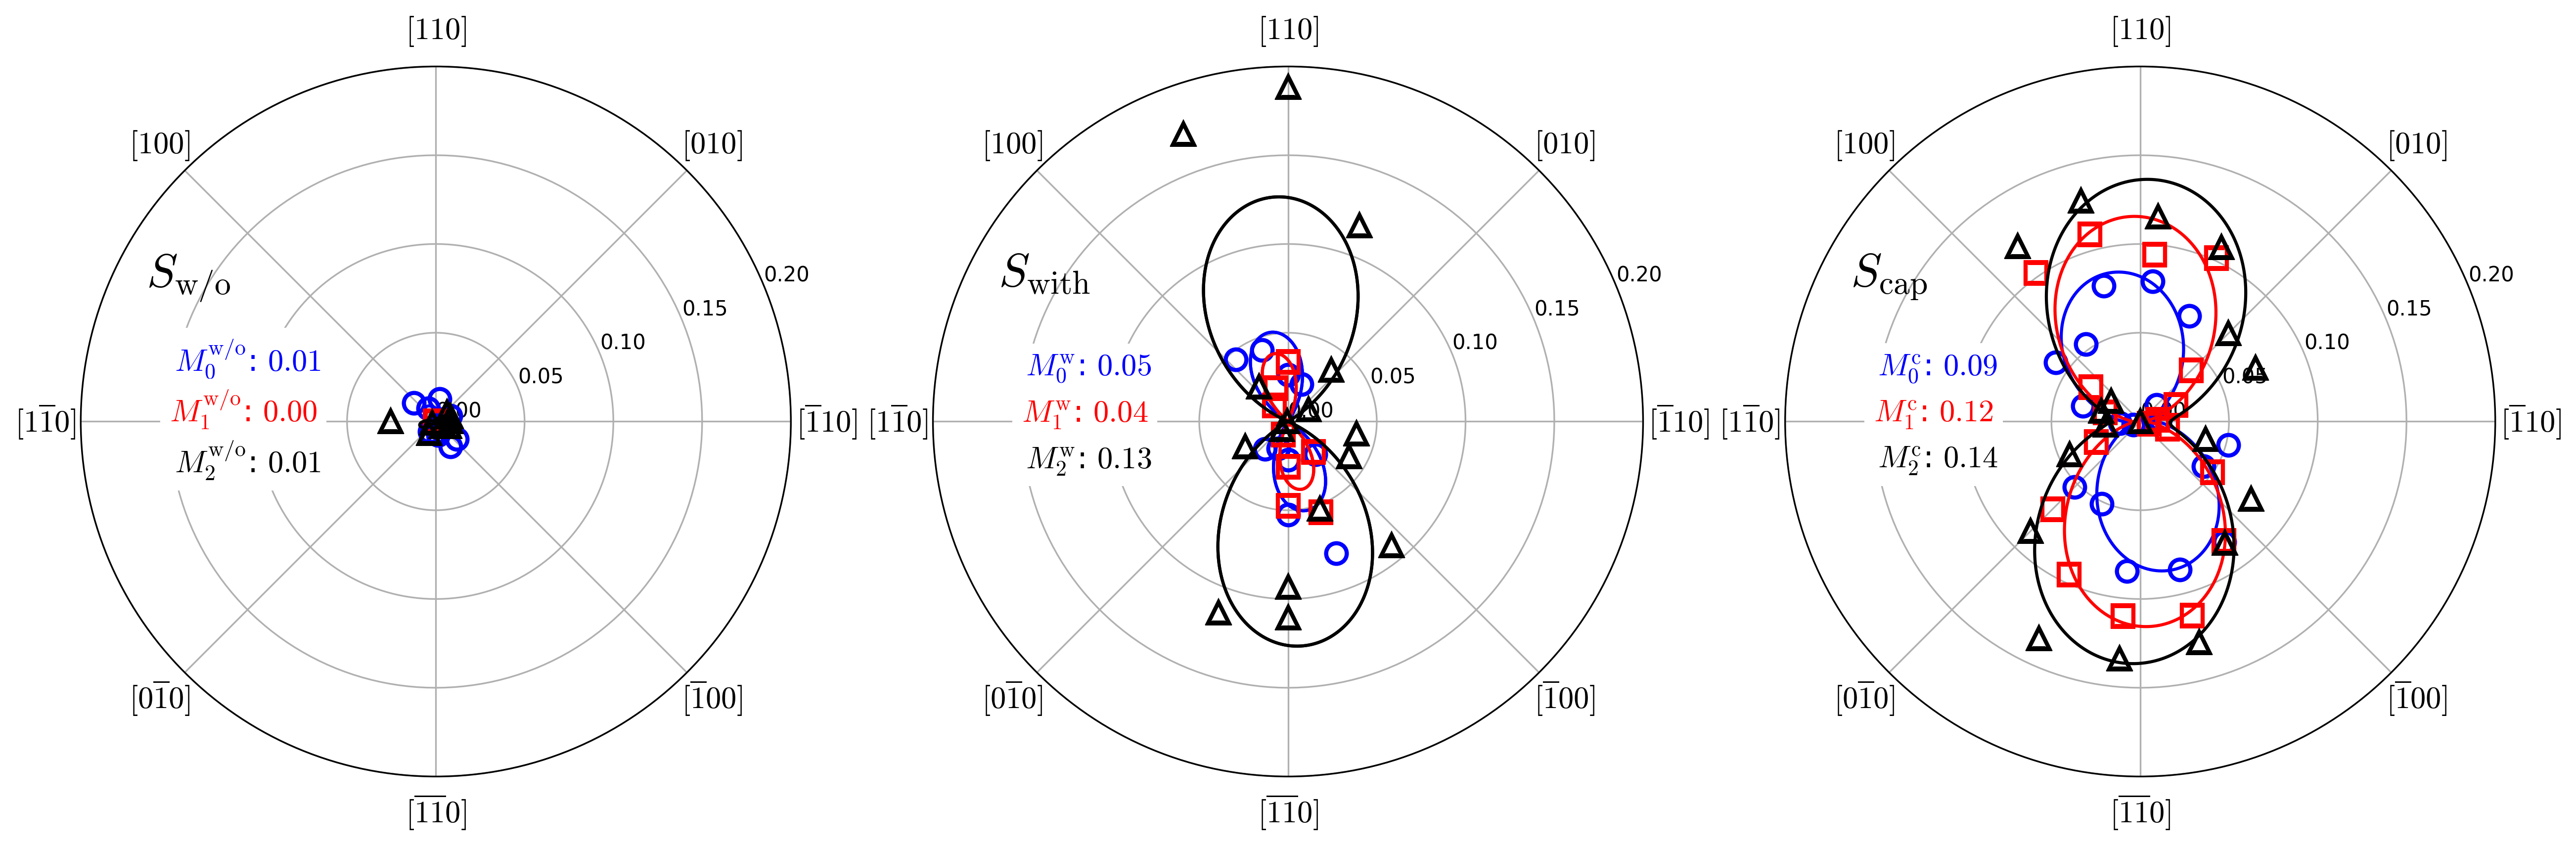
\includegraphics[width=1\linewidth]{/PL/polarization/POL_all}
	\caption{From left to right the polar graphs show $C(\theta)$ of samples ${S_\mathrm{w/o}}$, ${S_\mathrm{with}}$, and $\mathbf{S_\mathrm{cap}}$, respectively. Individual bands of PL spectra for each sample are represented by different symbols, consistently with previous labeling.}
	\label{fig:PL_pol_all}
\end{figure}

\newpage
\section{Time-resolved photoluminiscence}
%The measurements can be fitted to a double exponential decay function after convolution with the instrument response function (IRF) shown in the same graph
We have studied the dynamics of the recombination processes of our QD samples as a function of the emission energy, excitation density, and temperature. Each measured TRPL signal of samples $S_\mathrm{w/o}$ and $S_\mathrm{with}$ has been deconvoluted using a double mono-exponential (2ME) decay model
%
\begin{equation}
I(t)=A_1\exp(-t/\tau_1)+A_2\exp(-t/\tau_2),
\end{equation}
 %
 characterized by the amplitude $A_1$ ($A_2$) and the decay time $\tau_1$ ($\tau_2$) for the slow (fast) decay process.
 To reproduce TRPL signal in a maximum of PL intensity of sample $S_\mathrm{cap}$ triple mono-exponential (3ME) decay model was used.
 In order to compare the samples we introduce characteristic PL decay time $\tau_\mathrm{PL}$ as the weighted arithmetic mean of two (three) decay times for 2ME (3ME) model which corresponds to a decrease of PL intensity from its maximum value to the level of $1/\mathrm{e}$:
%
\begin{eqnarray}
\tau_\mathrm{PL}=\sum_{i=1}^{2 ( 3) } w_i\tau_i \label{eq:average_time}
\end{eqnarray}
%
where $w_i$ is weight [$w_i={A_i\cdot \tau_i }/{(\sum A_i \cdot \tau_i)}$] defined by fitting model.

Our analysis takes into account repumping of the slow component $\tau_1$ of the dynamics from previous pulses which leads to increase of \enquote{background} up to dark signal level as can be seen in Fig.~\ref{fig:TRPL_int_all_max}.


\subsection{Emission energy dependent TRPL}
%

%Using previous analysis the similar fast component $\tau_2$ in range 5 and 13~ns for all samples and $\tau_3$ around 25~ns for $S_\mathrm{w}$ and $S_\mathrm{cap}$ were found.

\begin{figure}[!ht]
	\centering
	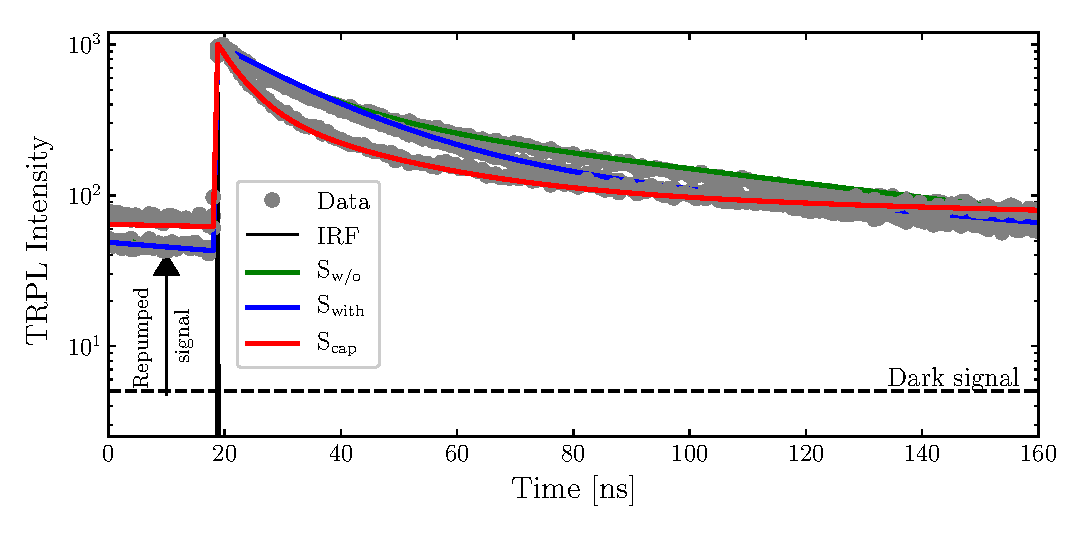
\includegraphics[width=1\linewidth]{/TRPL_after_Benito/intensity/TRPL_inMAX}
	\caption{Comparison of TRPL signals of our samples taken in maximum of PL intensity (grey circles) with corresponding multi-exponential fits (solid lines). The black line IRF represents laser scattering. Signal repumped from previous excitation pulses increases \enquote{background} from dark level (dashed line).}
	\label{fig:TRPL_int_all_max}
\end{figure}

% 3ME fits%
%
%In spite of similarity between our samples in $\tau_2$ of values in range 13 and 32~ns (for all samples) and $\tau_3$ smaller than 10~ns (only for $S_\mathrm{with}$ and $S_\mathrm{cap}$), $\tau_1$ of differs from 90~ns ($S_\mathrm{w/o}$) to 520~ns ($S_\mathrm{cap}$). To compare lifetimes across samples and emission energy where weights and number of mono-exponential decays varied, we use $\tau_\mathrm{PL}$. On the one hand, $\tau_\mathrm{PL}$ enlarges within one sample of decreasing energy, see Fig.~\ref{fig:TRPL_int_all}(a) where $\tau_\mathrm{PL}$ measured under the same conditions as a function of the emission energy for all three samples is summarized. On the second hand, that increases between samples from 74~ns ($S_\mathrm{w/o}$), over 164~ns ($S_\mathrm{with}$) to 364~ns ($S_\mathrm{cap}$). Decay times and appropriate weights of multi-exponential fits in the maximum of PL emission of each sample visualized in Fig.~\ref{fig:TRPL_int_all_max} are listed in Tab.~\ref{tab:TRPL_int_params}.
%

% 2ME fits%
%
Although to reproduce TRPL signal of samples $S_\mathrm{w/o}$ and $S_\mathrm{with}$ we used 2ME and $S_\mathrm{cap}$ was fitted by 3ME model, respectively, our samples show similarity in $\tau_2$ which we find in the range from 13 to 23~ns, but the samples differ in $\tau_1$ which vary from 90~ns for $S_\mathrm{w/o}$ up to 520~ns for $S_\mathrm{cap}$. The third decay time in TRPL signal of $S_\mathrm{cap}$ is around 5~ns.

To compare lifetimes across samples and emission energies we use $\tau_\mathrm{PL}$ incorporating varying weights and number of mono-exponential decays. On one hand, for each sample $\tau_\mathrm{PL}$ increases with decreasing emission energy, see Fig.~\ref{fig:TRPL_int_all}~(a) where we summarize $\tau_\mathrm{PL}$ measured under the same conditions as a function of the emission energy for all three samples. Interestingly, while $\tau_\mathrm{PL}$ is changing similarly with energy for most of the samples, for emission of $S_\mathrm{cap}$ at 1.77~eV we have found much slower $\tau_\mathrm{PL}$ (around 1~$\mu$s).

 On the second hand, $\tau_\mathrm{PL}$ increases among samples: 74~ns ($S_\mathrm{w/o}$), 85~ns ($S_\mathrm{with}$), and 364~ns ($S_\mathrm{cap}$). Decay times and appropriate weights of multi-exponential fits in the maximum of PL emission of each sample visualized in Fig.~\ref{fig:TRPL_int_all_max} are also listed in Tab.~\ref{tab:TRPL_int_params}.

\begin{figure}[!ht]
	\centering
	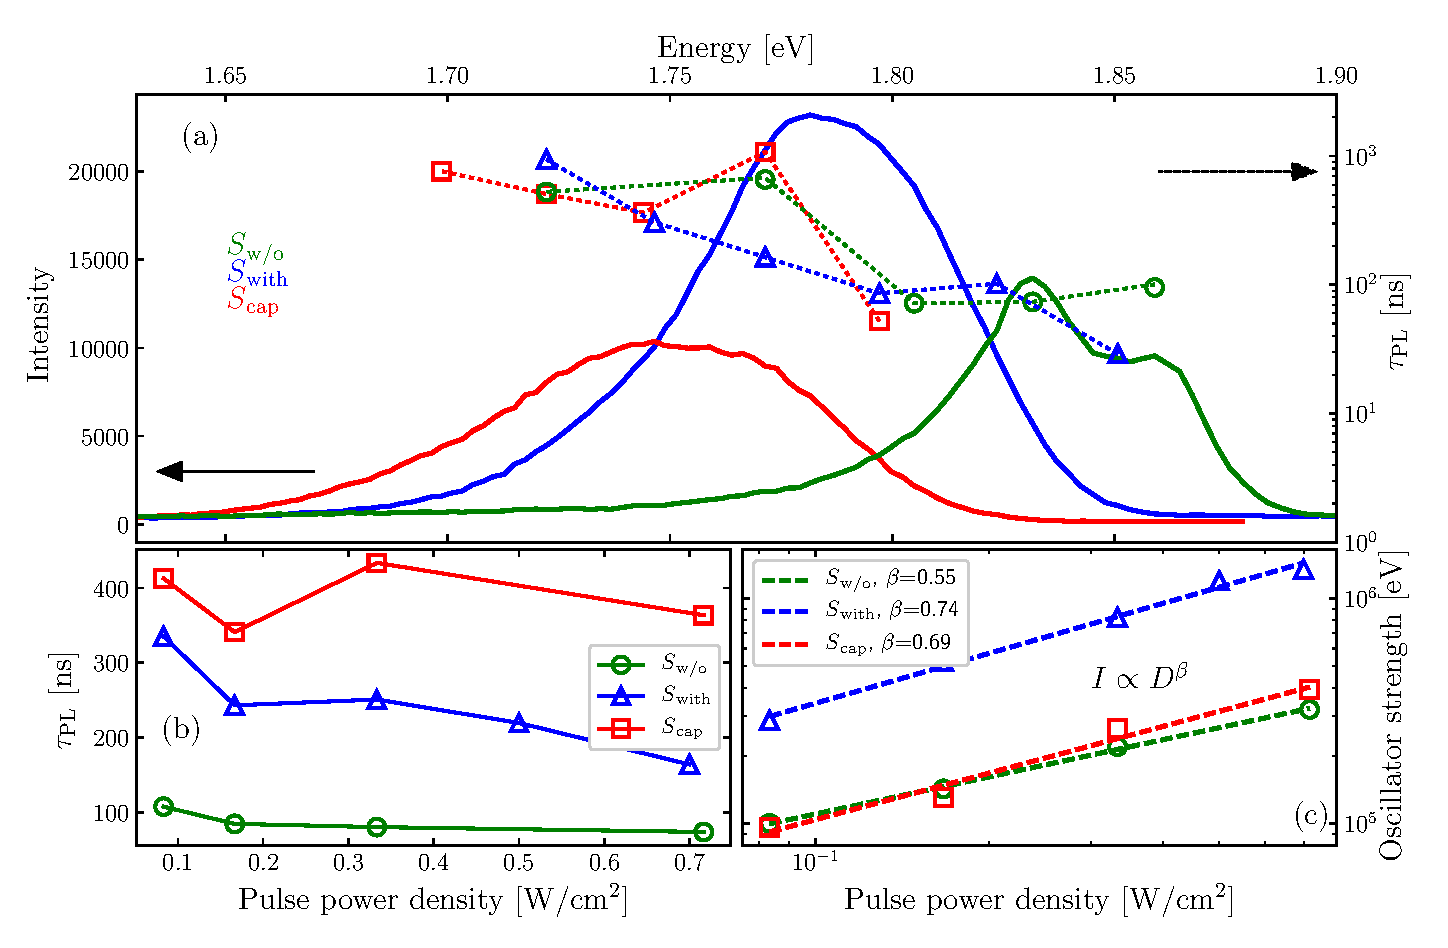
\includegraphics[width=1\linewidth]{/TRPL_after_Benito/intensity/porovnani_vzorku_maximum_int_after_Benito_log}
	\caption{(a) Decay times $\tau_\mathrm{PL}$ (symbols) for the studied samples as a function of the emission energy measured at the temperature of 15~K and pumping power of 0.7~W/cm$^2$. Appropriate PL spectra (solid lines) are added for better orientation. Panel~(b) depicts $\tau_\mathrm{PL}$ in the maximum of the PL signal and panel~(c) $\tau_\mathrm{PL}$ that for the integrated PL intensity in whole measured spectral range as a function of excitation power density.}
	\label{fig:TRPL_int_all}
\end{figure}
%
%
\begin{table}
	\centering
	\caption{Summary of the multi-exponential fitting parameters of our samples in the maximum of PL intensity.}
	\begin{tabularx}{0.9\textwidth}{cCCcc}
		\toprule
		sample & $\tau_1/w_1$ [ns/\%]&  $\tau_2/w_2$ [ns/\%]  & $\tau_3/w_3$ [ns/\%] & $\tau_\mathrm{PL}$ [ns] \\ 	
		\midrule
		\midrule
		$S_\mathrm{w/o}$& 91.42/77 & 13.23/23 & -& 73.7\\
		\midrule
		%$S_\mathrm{with}$& 360.7/41 &  32.20/46 &9.76/13&  164.0\\ 3ME fit
		$S_\mathrm{with}$& 136.2/57 &  17.89/43 &-&  85.3\\
		\midrule
		$S_\mathrm{cap}$ & 518.8/69 &  23.11/21 &4.91/10&  363.7\\ 	
		\bottomrule
	\end{tabularx}\label{tab:TRPL_int_params}
\end{table}
%
%
%





\newpage
\subsection{Excitation intensity dependent TRPL}
%
The excitation density of the pulse laser was varied in the range 0.08--0.7~W/cm$^2$, the optical response was in linear regime in the whole varied excitation range for each sample, see Fig.~\ref{fig:TRPL_int_all}~(c). Thereafter, the measured TRPL signal has been deconvoluted by multi-exponential decay model. %, e.~g., Fig.~\ref{fig:TRPL_int_w} depicts TRPL signal in the maximum of PL spectra of $S_\mathrm{with}$). 

Let us start with TRPL of sample $S_\mathrm{w/o}$ where $\tau_\mathrm{PL}$ in the emission energy range from 1.80 to 1.86~eV is constant at 80~ns which leads us to substitute the dynamical processes for this energy interval by investigation of decay times in the maximum of PL intensity, see Fig.~\ref{fig:TRPL_int_wo}. We observe a decrease of decay times for $\tau_1$ from 130 to 90~ns and for $\tau_2$ from 30 to 13~ns, respectively.

The decrease of decay times point to indirect transition of electrons from X band to heavy holes in $\Gamma$ band of GaAs, moreover, weight of the processes stays the same irrespective of pumping which is probably connected with character of $M_1^\mathrm{w/o}$ and $M_2^\mathrm{w/o}$ transitions. As previously discussed in Sec.~\ref{Sec:PL_int_wo} we conclude that $M_1^\mathrm{w/o}$ is a phonon replica of $M_2^\mathrm{w/o}$. The decay times $\tau_1$ and $\tau_2$ correspond to bands $M_2^\mathrm{w/o}$ and $M_1^\mathrm{w/o}$, respectively. The previous assignment will be discussed in Sec.~\ref{chap:TRPL_temp}.
%We refer to temperature resolved TRPL in Sec.~\ref{chap:TRPL_temp} where the nature of $\tau_1$ and $\tau_2$ will be discussed. %tau1 je bezfonon, tau2 je fonononova

%This behaviour arrived us to Because the faster process $\tau_2$ was observed across our samples and emission energy, we assume that it comes from the substrate. (Je to dobre s tim typem II v rec. prostoru?)

%We observe a decrease of the fast decay component with increasing excitation density as shown in Fig.~\ref{fig:TRPL_int_w}(b)--(c), which is in agreement with behaviour of type-II nanostructures observed elsewhere~\citep{Ledentsov_prb1995_intmodel,Gu_prb2005_TRPLtype2,Manna_apl2012_TRPLtype2,Zaitsev_prb2007}. At higher excitation intensity, a larger carrier concentration of the photogenerated electron-hole pairs results in band bending, hence a stronger overlap of electron-hole wave-functions, and thus a faster decay.
%

\begin{figure}
	\centering
	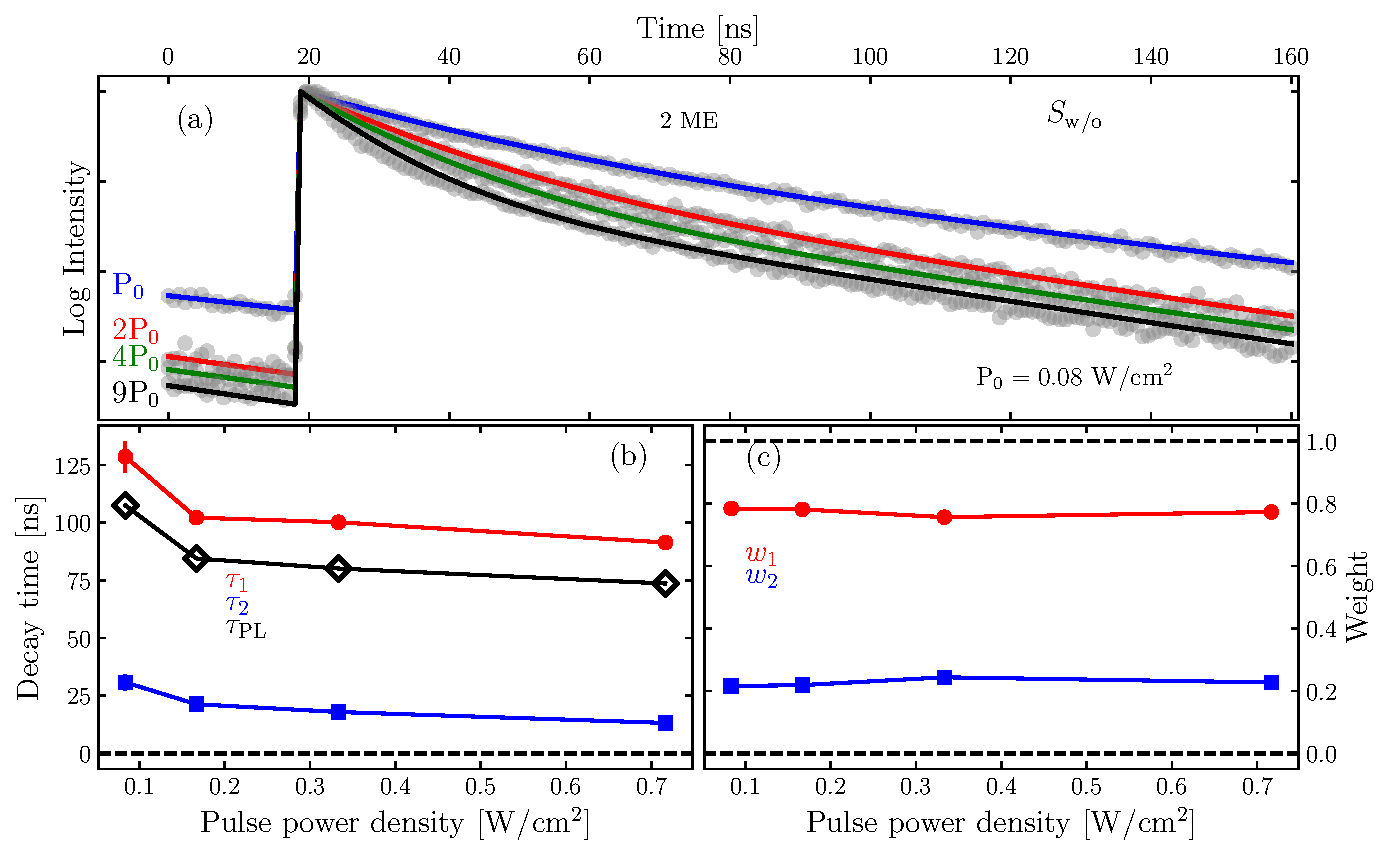
\includegraphics[width=1\linewidth]{/TRPL_after_Benito/intensity/12027_TRPL_677nm_int}
	\caption{(a) TRPL measured at 15~K as a function of excitation density (grey circles) and its deconvolution by 2ME model (solid lines) at the energy where maximum of band $M^1_\mathrm{w/o}$ intensity for sample $S_\mathrm{w/o}$ occurs. (b) Fitted decay times $\tau_1$ (red circles), $\tau_2$ (blue squares) and characteristic time $\tau_\mathrm{PL}$ (black diamonds) as a function of excitation density. Corresponding weights are shown in panel (c).}
	\label{fig:TRPL_int_wo}
\end{figure}

%Samples $S_\mathrm{with}$ and $S_\mathrm{cap}$ were fitted by 3ME model with very similar behaviour of $\tau_2$ as in sample $S_\mathrm{w/o}$, i.~e., a slight decrease in decay times and the same difference in weights. Moreover, $\tau_2$ is in range between 20 and 35~ns which is comparable with $\tau_2$ in $S_\mathrm{w/o}$. But, interestingly, $\tau_1$ is independent on excitation intensity or slightly increasing with that for both $S_\mathrm{with}$ and $S_\mathrm{cap}$ samples and it is much longer than other decay times: $\tau_1$ is between 330~ns (450~ns) and 380~ns (540~ns) for $S_\mathrm{with}$ ($S_\mathrm{cap}$). 



Sample $S_\mathrm{with}$ was deconvoluted by 2ME and $S_\mathrm{cap}$ by 3ME model see panels (a) in Figs.~\ref{fig:TRPL_int_w}--\ref{fig:TRPL_int_c}. Similar decrease in decay times from 28 to 20~ns as for sample $S_\mathrm{w/o}$ is observed. This process has been previously discussed also for $S_\mathrm{w/o}$ and it is connected with radiative emission from GaAs layer.
%

Because time response of the emission from $S_\mathrm{with}$ characterized by $\tau_\mathrm{PL}$ in the spectral range from 1.77 to 1.82~eV is similar, we again describe the dynamics of $S_\mathrm{with}$ for energies in the maximum of PL intensity. The slower process labelled as $\tau_1$ decreases with excitation power. 
%
{\color{red}{(TADY se musime domluvit, co to teda ma byt. Navrhy PS: 1) ovlivnena ta GaAs vrstva - na tomto vzorku by vubec nebyly tecky a jen pri snaze je narust, by se rozsirila tloustka te GaAs vrstvy a prineslo by to do ni trosku india. Coz by posunulo PL k nizsim energiim? a mohlo by to protahnout rakombinacni cas.

2) InGaAs QD typu II s dlouhou dobou zivota, ktera se ale ovlivnuje s excitaci a tim se zrychluje. ) }}
{\color{green}{(Vypoctum pro maly obsah Sb a In vyhovovala spis varianta 1.) ale jeste se to musi proverit a prepocitat.) }}
%
\begin{figure}
	\centering
	%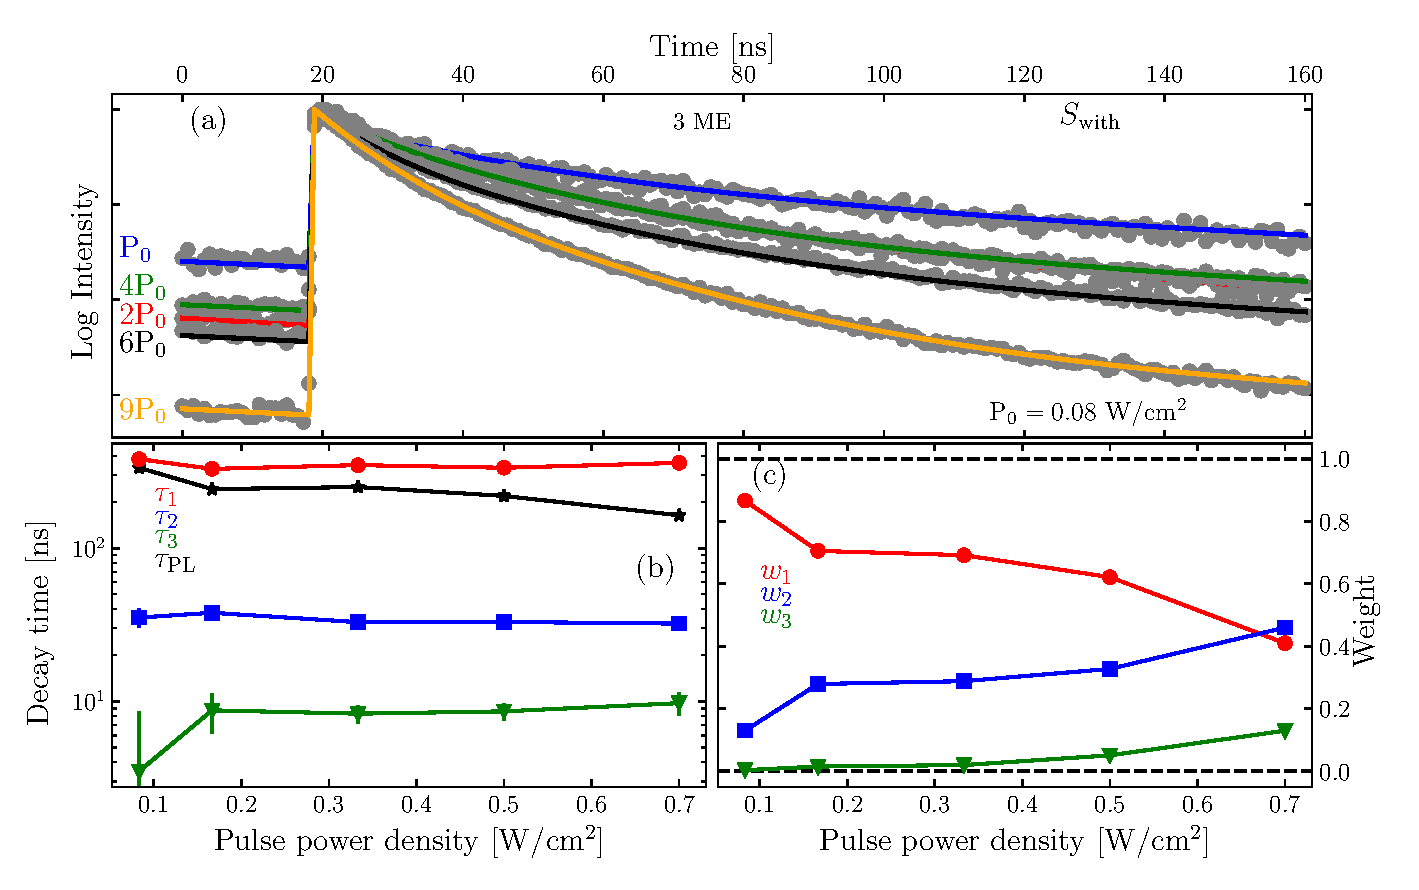
\includegraphics[width=1\linewidth]{/TRPL_after_Benito/intensity/12040_TRPL_700nm_int} %3ME fit
	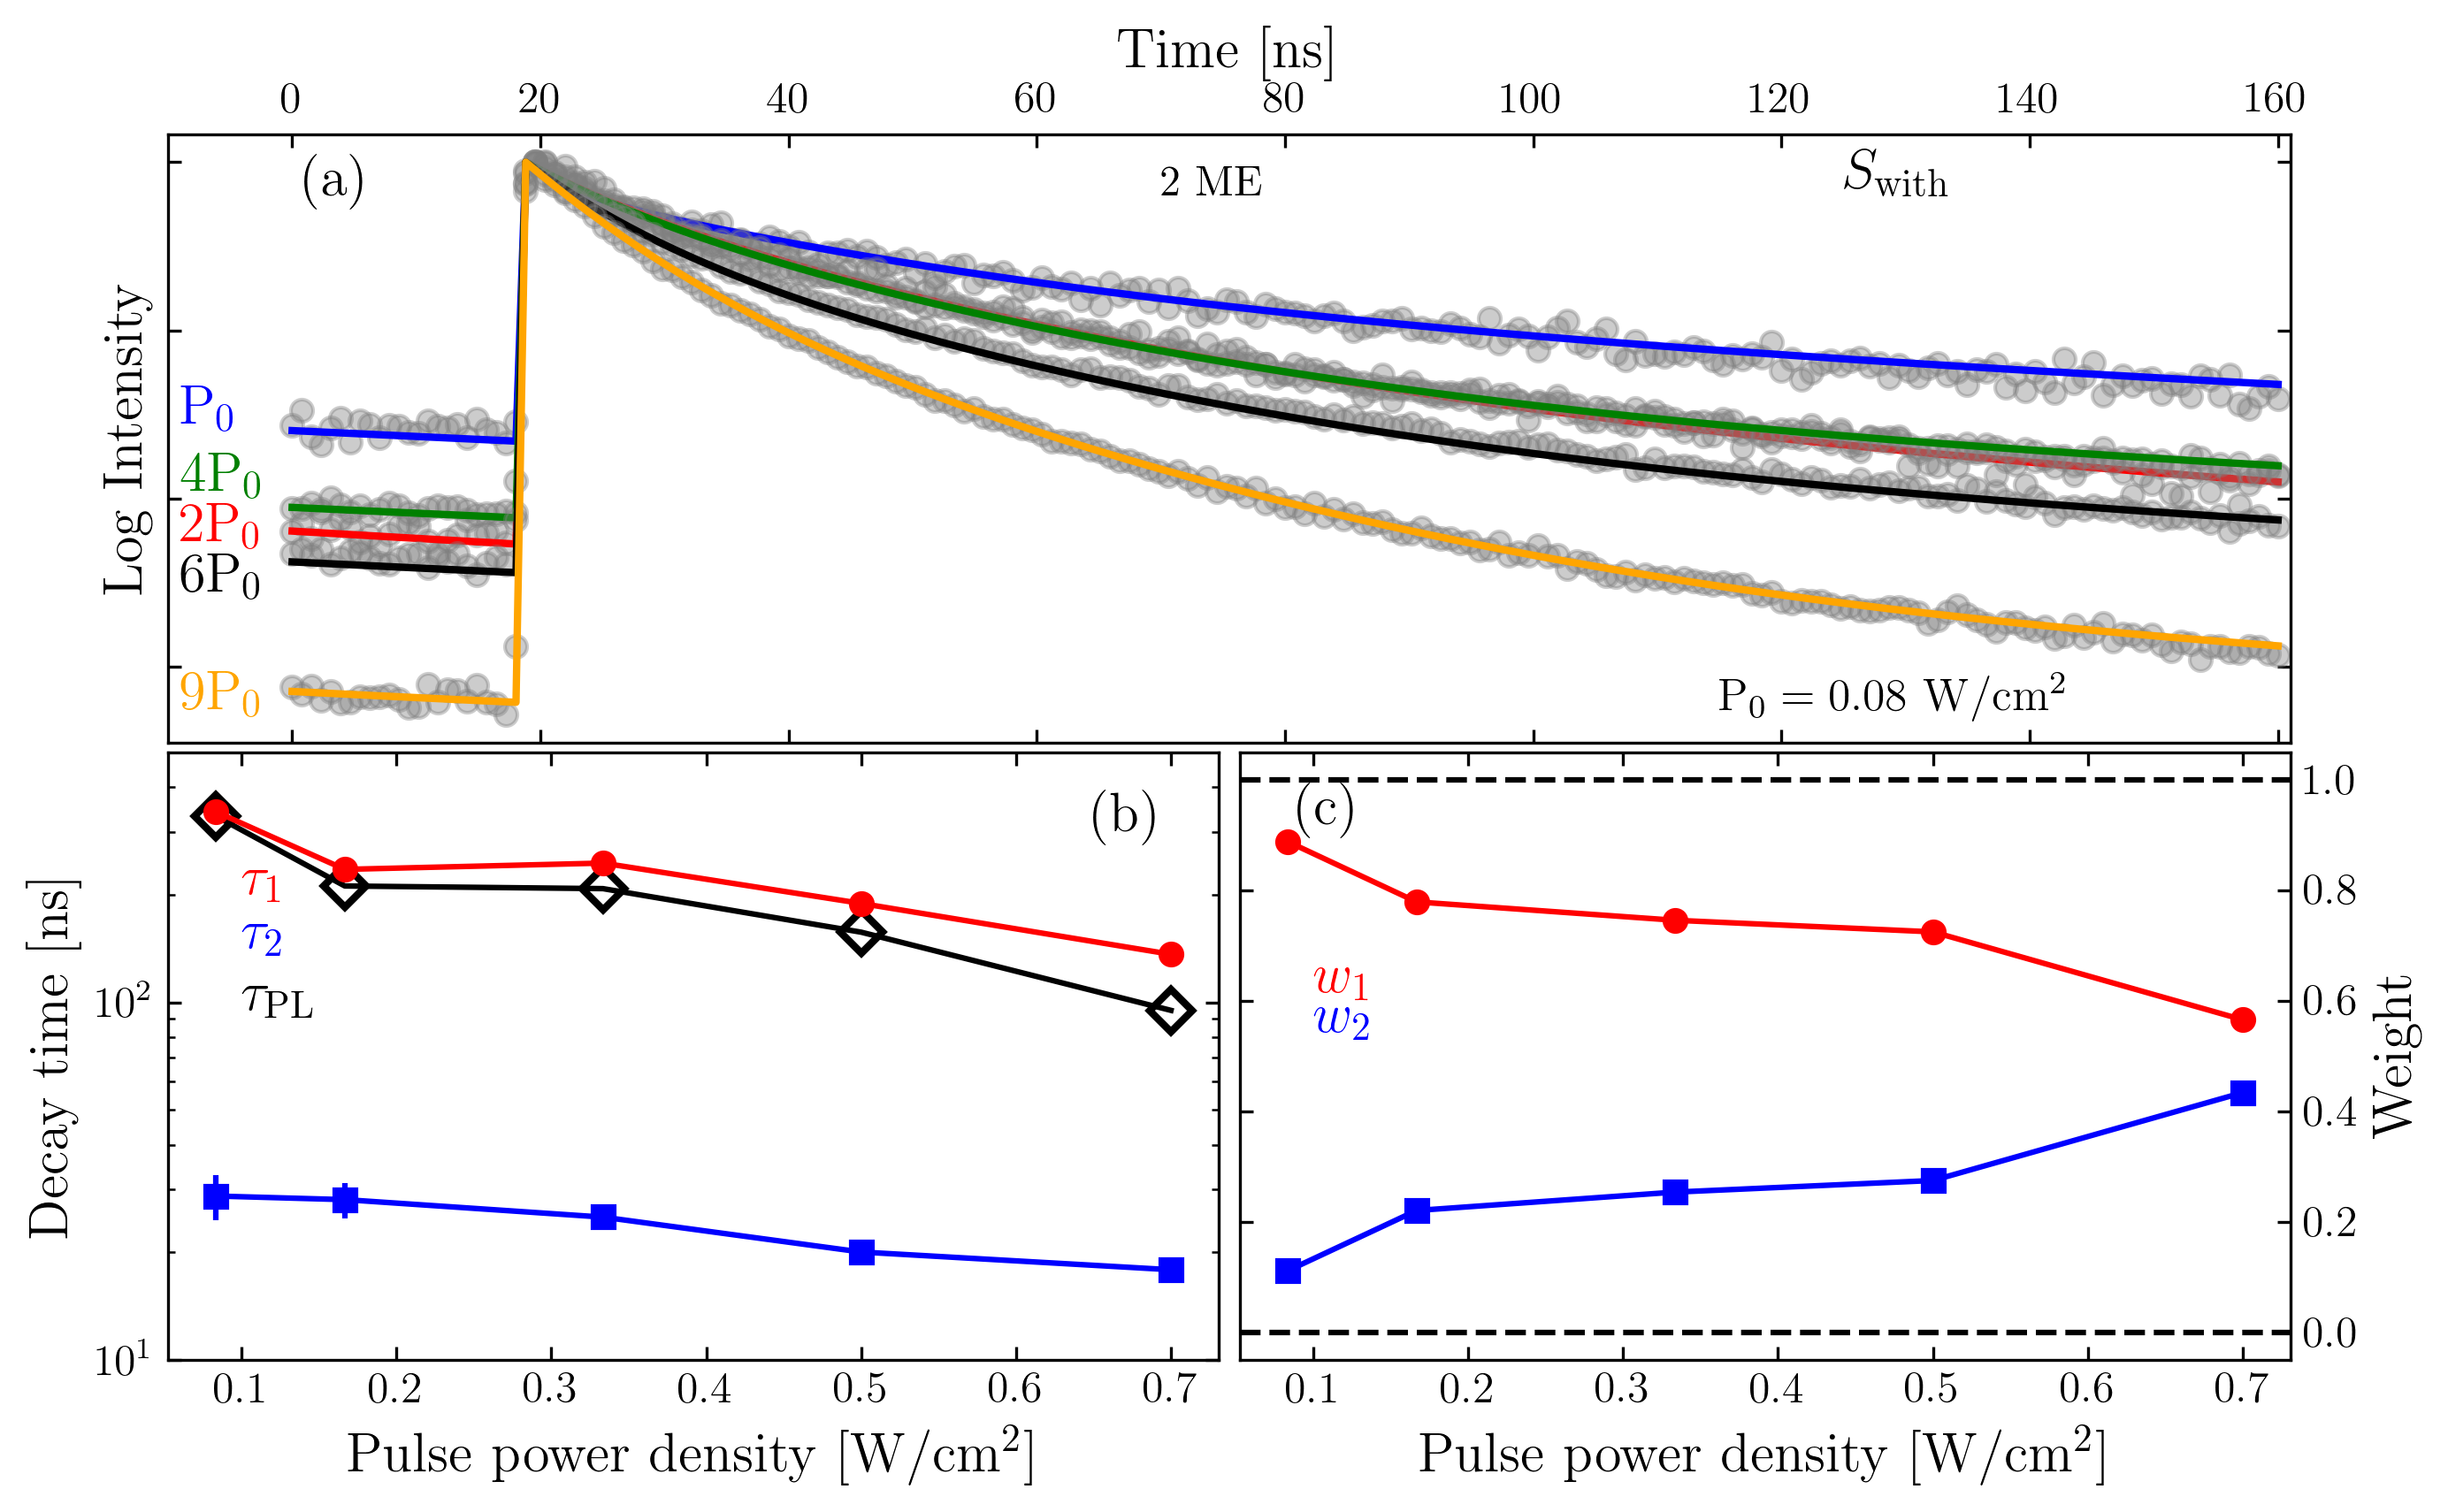
\includegraphics[width=1\linewidth]{/TRPL_after_Benito/intensity/12040_TRPL_690-700nm_int_2tau} %2ME fit
	\caption{TRPL signal of $S_\mathrm{with}$ deconvoluted similarly as in Fig.~\ref{fig:TRPL_int_wo}.}
	\label{fig:TRPL_int_w}
\end{figure}



On the other hand, $\tau_\mathrm{PL}$ of sample $S_\mathrm{cap}$ is slower for the high energy side of PL spectrum (energy around 1.77~eV) than for lower energies of PL and also compared to other samples. For this reason we investigated both energy intervals individually. Analysis in {Figs.~\ref{fig:TRPL_int_c}--\ref{fig:TRPL_int_c_L}} by 3ME model shows that in both there are two comparable processes $\tau_2$ and $\tau_3$ present. While for increasing excitation power $\tau_2$ decreases and it is most probably associated with the dynamics of GaAs layer, $\tau_3$ stays almost constant at 5~ns and presents with type-I nature of the confinement~\cite{Heitz_TRPL_typeI_PRB97}. We attribute the latter to transitions between electrons from $\Gamma$ band to holes from the same band, see also Fig.~\ref{fig:TRPL_int_c_theory}.%{\color{red}{(máš nějakou referenci, ja nemuzu nic najit)}}{\color{green}{(zkus treba: https://onlinelibrary.wiley.com/doi/pdf/10.1002/pssc.200881512 https://aip.scitation.org/doi/10.1063/1.2964191 a samozrejme nas stary znamy, ktery prijede pristi tyden: https://journals.aps.org/prb/pdf/10.1103/PhysRevB.56.10435 )}}





%The processes characterized by $\tau_1$ and $\tau_3$ are presented only on samples $S_\mathrm{with}$ and $S_\mathrm{cap}$, as can be seen in panels (b) in Figs.~\ref{fig:TRPL_int_w}--\ref{fig:TRPL_int_c}, stay almost constant ($\tau_3=8$~ns) or only slightly increase ($\tau_1$) with increasing excitation power which is behaviour observed for type-I nanostructures. (máš nějakou referenci, ja nemuzu nic najit)


%Process characterized by $\tau_3$ is presented only on samples $S_\mathrm{with}$ and $S_\mathrm{cap}$ and stays constant with increasing excitation power at 8~ns.

Interestingly, time $\tau_1$ corresponding to the third process is increasing with excitation intensity for both low and high part of PL of $S_\mathrm{cap}$ and it is also much longer than other decay times: $\tau_1$ is between 330~ns (650~ns) and 380~ns (2.8~$\mu$s) at 1.75~eV (1.77~eV). Note, however, that the weight of processes characterized by decay time $\tau_1$ for both $S_\mathrm{with}$ and $S_\mathrm{cap}$ decreases with increasing excitation.


Finally, processes characterized by decay times $\tau_1$ and $\tau_3$ and their evolutions with intensity of excitation laser were compared to theoretical predictions obtained by SSCCI method by the supervisor. The process associated with $\tau_1$ was identified as a radiative transition between electrons originating from $L$ and holes from $\Gamma$-point of the reciprocal space. On the other hand, a radiative transition from $\Gamma$ electrons can describe the process characterized by $\tau_3$. For comparison of SSCCI calculations and experimentally obtained decay times as a function of excitation power see Fig.~\ref{fig:TRPL_int_c_theory}.


\begin{figure}
	\centering
	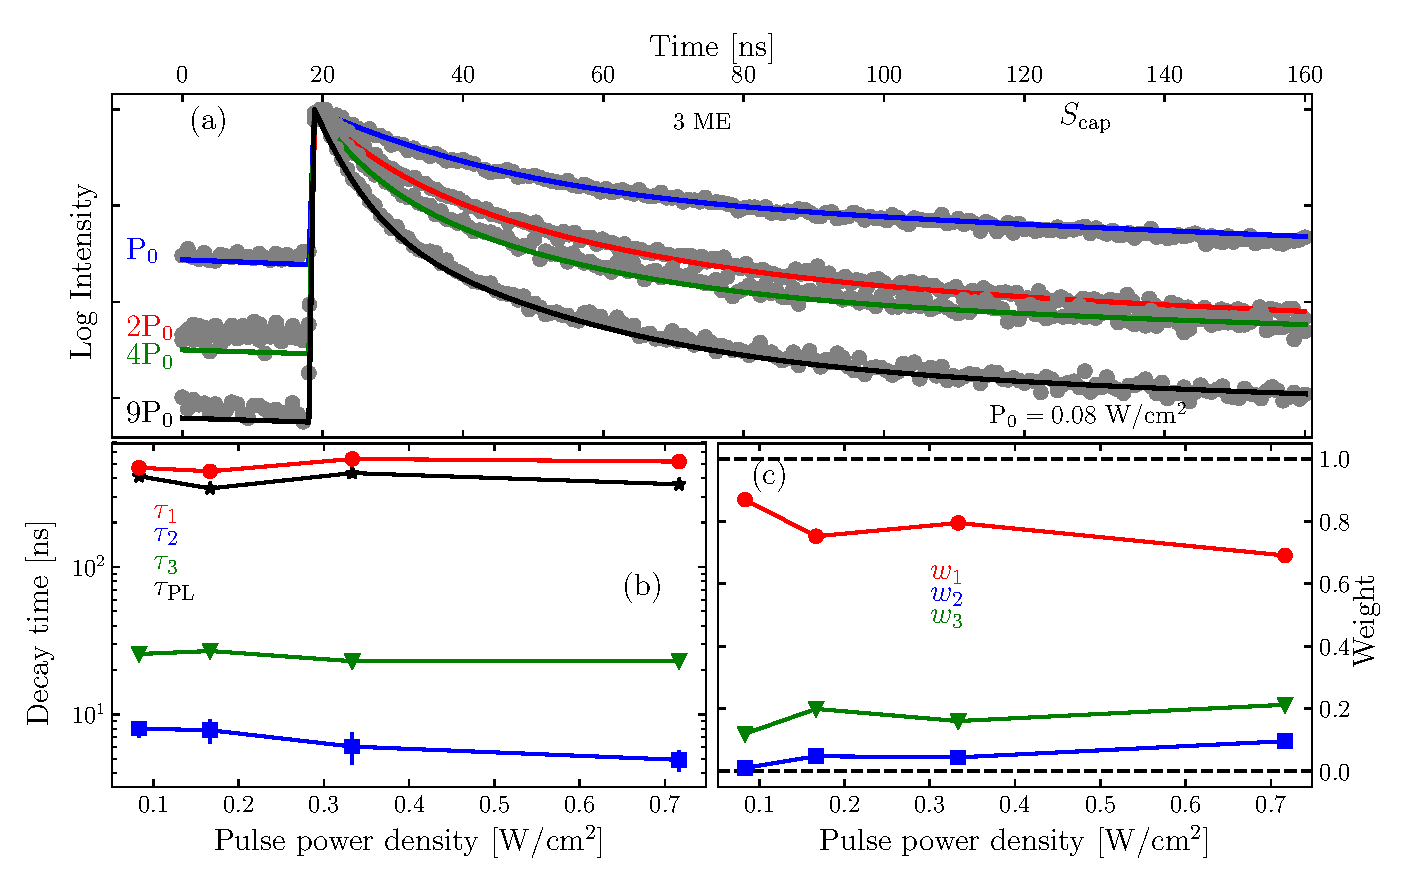
\includegraphics[width=1\linewidth]{/TRPL_after_Benito/intensity/12021_TRPL_710nm_int}
	\caption{(a) Deconvolved TRPL signal measured at 15~K by 3ME model (solid lines) as a function of excitation density (grey circles) at the energy corresponding to the maximum of band $M_1^\mathrm{c}$ (1.75~eV) for sample $S_\mathrm{cap}$. (b)~Fitted decay times $\tau_1$ (red circles), $\tau_2$ (blue squares), $\tau_3$ (green triangles), and characteristic time $\tau_\mathrm{PL}$ (black diamonds) as a function of excitation power density. Corresponding weights are shown in panel~(c).}
	\label{fig:TRPL_int_c}
\end{figure}

\begin{figure}
	\centering
	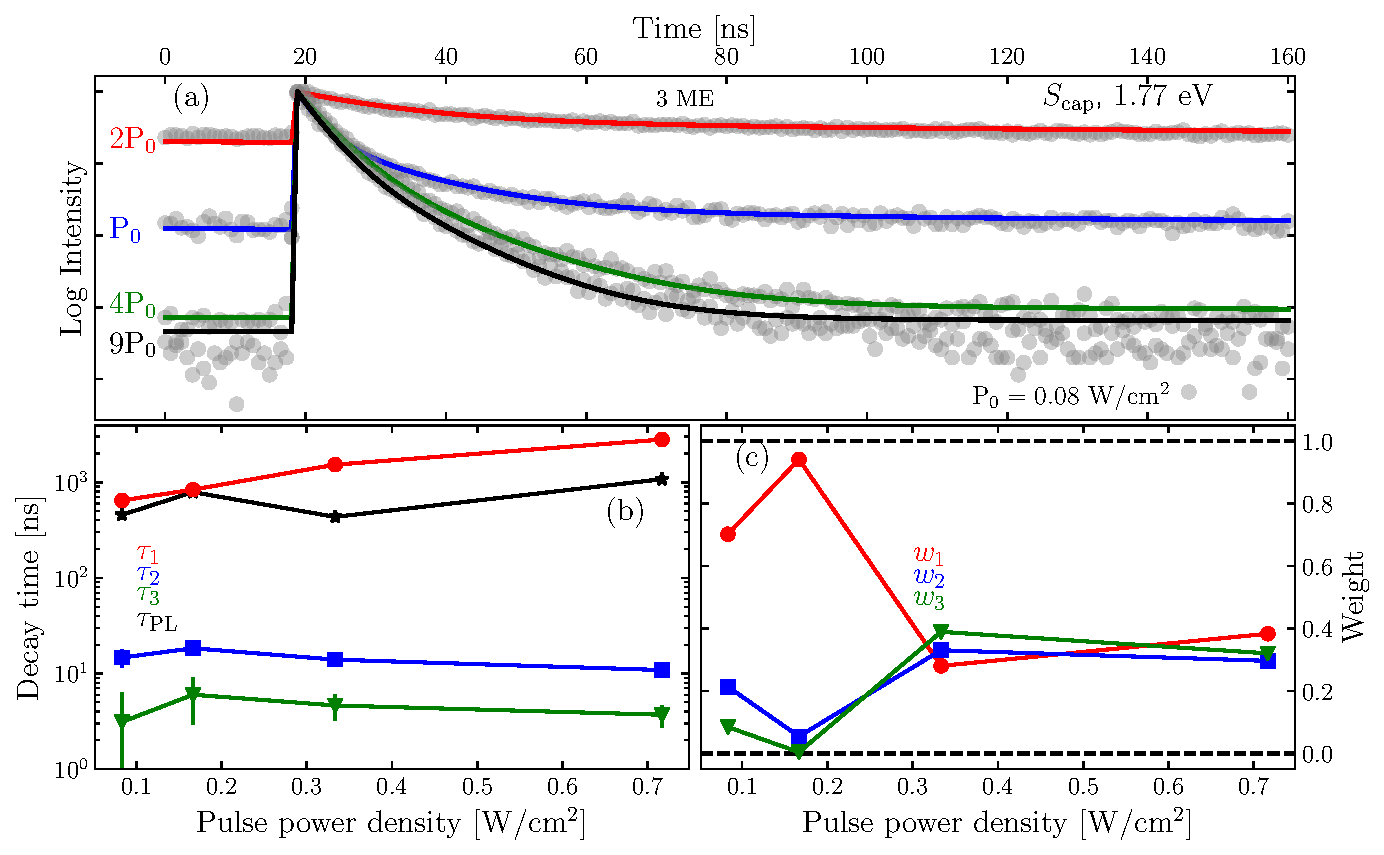
\includegraphics[width=1\linewidth]{/TRPL_after_Benito/intensity/12021_TRPL_700nm_int}
	\caption{Similar analysis as in Fig.~\ref{fig:TRPL_int_c} but obtained at energy of 1.77~eV.}
	\label{fig:TRPL_int_c_L}
\end{figure}

\begin{figure}
	\centering
	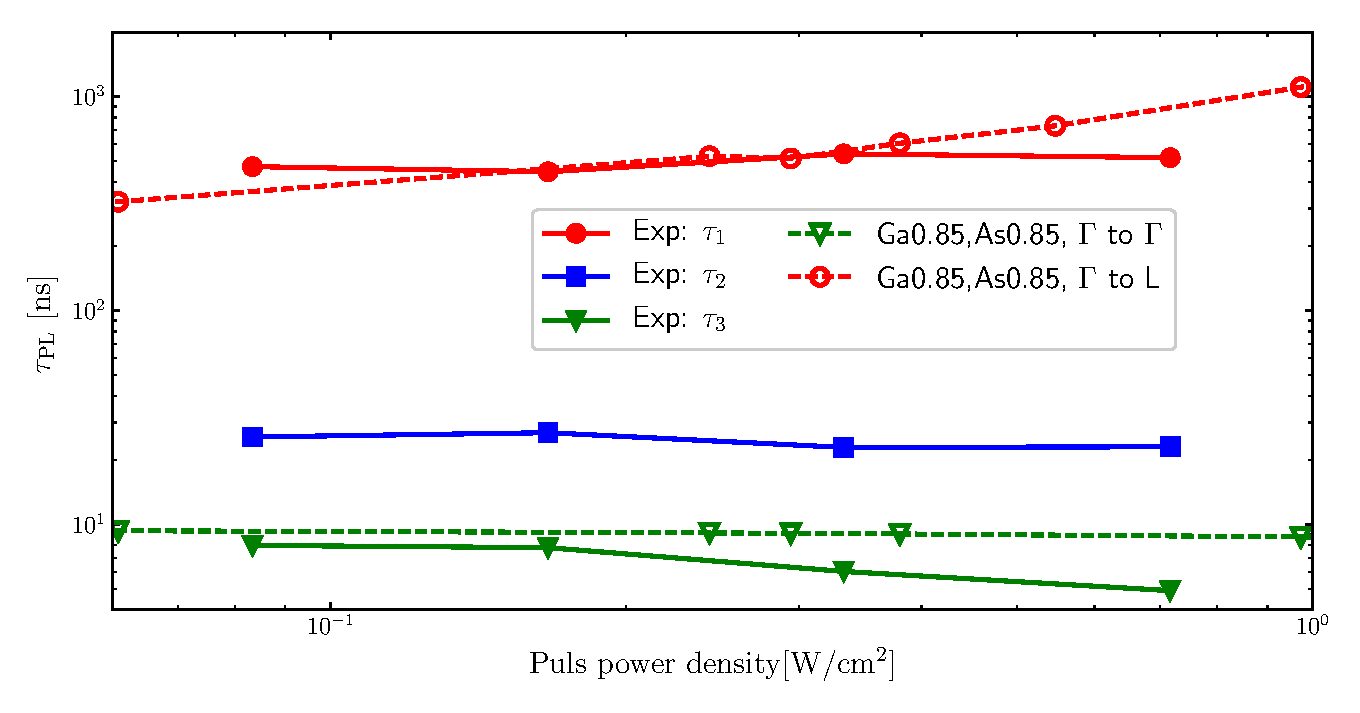
\includegraphics[width=1\linewidth]{/TRPL_after_Benito/intensity/12040_1107_TRPL_int_vs_theory_LandGamma}
	\caption{Experimental decay times obtained by 3ME fit of TRPL signal at 1.75~eV of $S_\mathrm{cap}$ (full symbols) as a function of excitation intensity and SSCCI with single-particle bases calculated by $1\times8$ $\mathbf{k\cdot p}$ and $8\times8$ $\mathbf{k\cdot p}$ (dashed lines).}
	\label{fig:TRPL_int_c_theory}
\end{figure}

%Other samples given in appendix~\ref{chapter:appendix_TRPL_int} show similar behaviour and with comparable $\tau_\mathrm{PL}$ at low excitation power. However, $\tau_\mathrm{PL}$ of samples with QDs is approximately twice as small, see Fig.~\ref{fig:TRPL_int_all}(b).





\clearpage
\subsection{Temperature dependent TRPL}
\label{chap:TRPL_temp}
%
TRPL variations with temperature are shown in Figs.~\ref{fig:TRPL_temp_wo}-\ref{fig:TRPL_temp_c} and are deconvoluted again by 2ME model for $S_\mathrm{w/o}$ and $S_\mathrm{with}$ and 3ME model for $S_\mathrm{cap}$, respectively. As can be seen in Fig.~\ref{fig:TRPL_temp_w}~(b) the resulting decay time $\tau_2$ of sample $S_\mathrm{with}$ increases up to the temperature of 30~K and thereafter progressively reduce which is characteristic of the appearance of thermally activated escape paths~\citep{Manna_apl2012_TRPLtype2}. Contrary to $\tau_2$ on sample $S_\mathrm{with}$, on $S_\mathrm{w/o}$ and $S_\mathrm{cap}$ the reduction of the decay times begins already at lowest temperatures without an increase at the beginning.

Similarly as in power series, the weight of the slower component contribution $\tau_1$ becomes smaller with increasing temperature.
% and around 100~K.
%
\begin{figure}
	\centering
	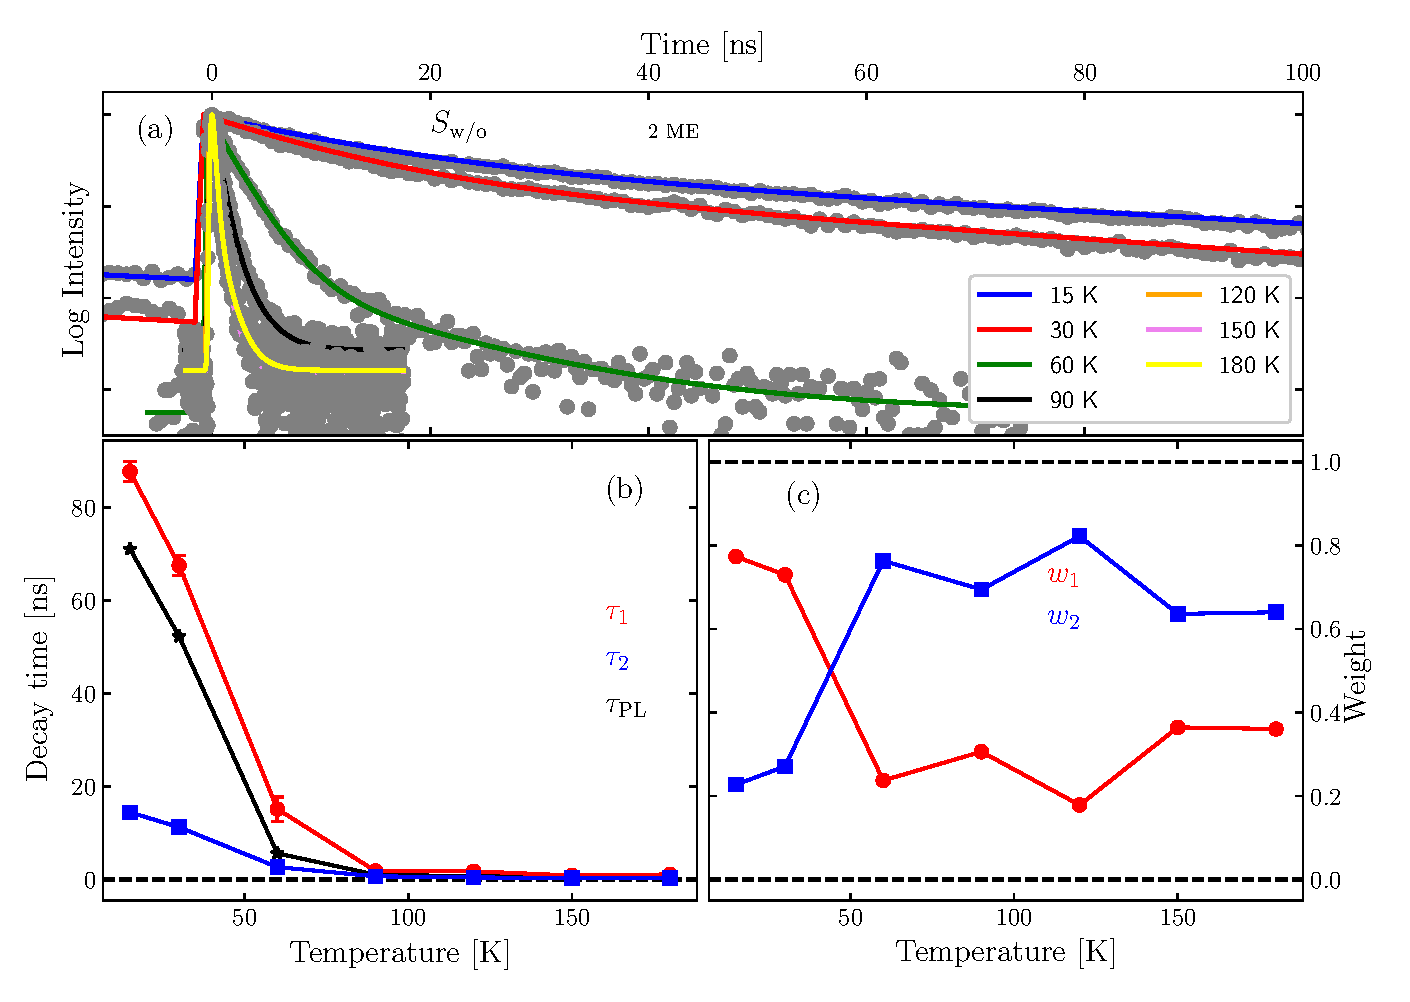
\includegraphics[width=0.9\linewidth]{/TRPL_after_Benito/temperature/12027_TRPL_677nm_temp}
	\caption{(a) Experimental TRPL at pumping power of 0.3~W/cm$^2$ as a function of temperature (grey circles) and its deconvolution by 2ME model (solid lines) at the maximum of PL signal for sample $S_\mathrm{w/o}$. (b) Deconvolved decay times ($\tau_1$: red circles; $\tau_2$: blue squares) and characteristic time $\tau_\mathrm{PL}$ (black diamonds) as a function of temperature. Corresponding weights are shown in panel (c).}
	\label{fig:TRPL_temp_wo}
\end{figure}
%
\begin{figure}
	\centering
	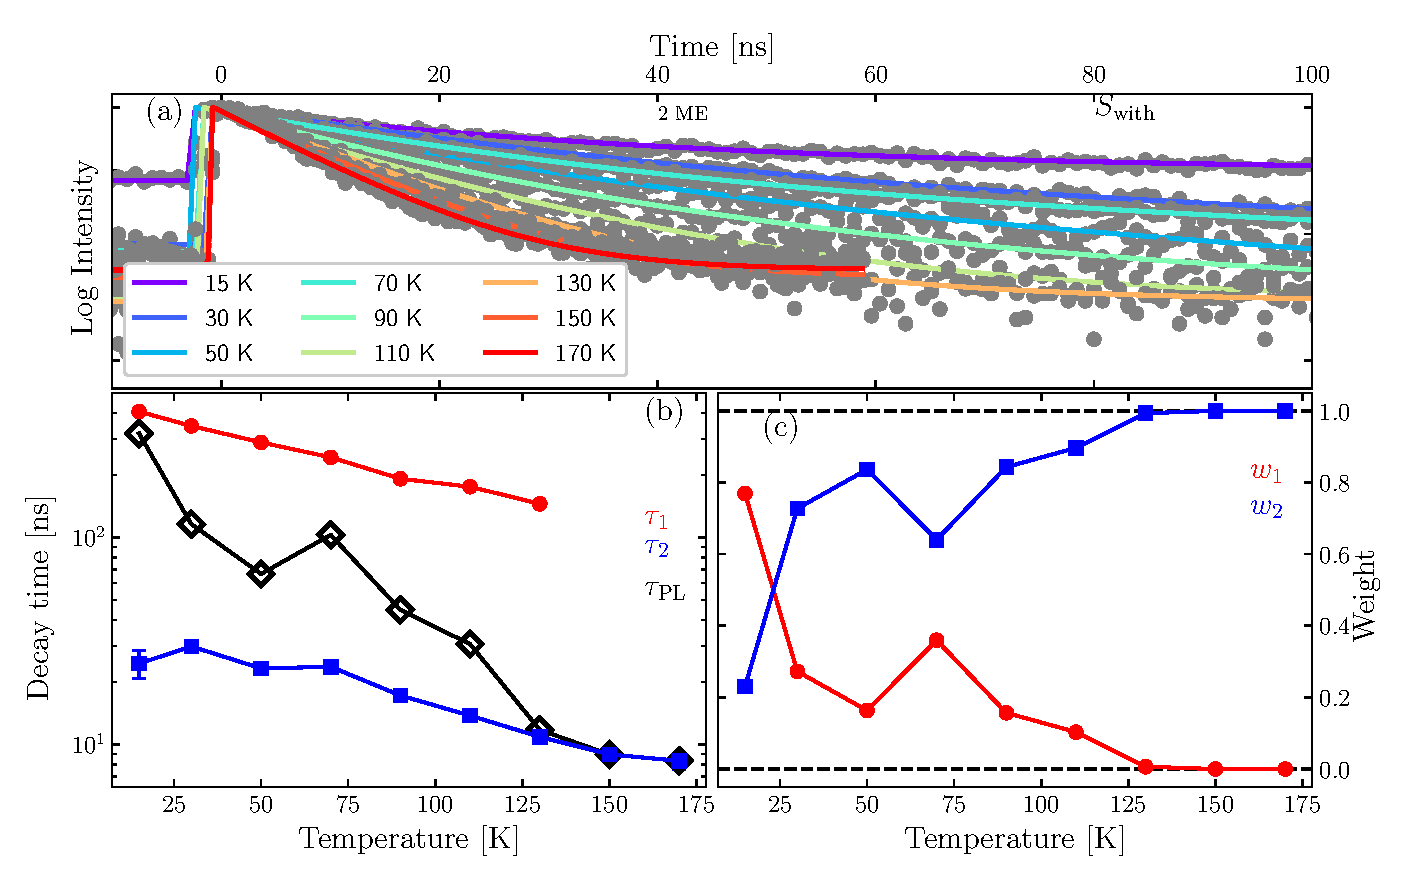
\includegraphics[width=0.9\linewidth]{/TRPL_after_Benito/temperature/12040_TRPL_690-700_temp_2tau}
	\caption{TRPL signal as a function of temperature at the maximum of PL for sample $S_\mathrm{with}$ similarly commented as in Fig.~\ref{fig:TRPL_temp_wo}.}
	\label{fig:TRPL_temp_w}
\end{figure}
%

If we assume similarly as in Ref.~\citep{t_alvarez} that at 15~K the only loss mechanism is radiative recombination, then the radiative $\tau_\mathrm{R}$ and non-radiative $\tau_\mathrm{NR}$ decay times can be extracted from the slow decay time $\tau_1$ by
%
\begin{equation}
\tau_\mathrm{R}=\frac{I_0}{I_\mathrm{PL}(T)}\tau_1 \label{eq:tau_R_fromtau1}
\end{equation}
and
\begin{equation}
\frac{1}{\tau_1}=\frac{1}{\tau_\mathrm{R}} + \frac{1}{\tau_\mathrm{NR}}
\end{equation}
%
\begin{figure}
	\centering
	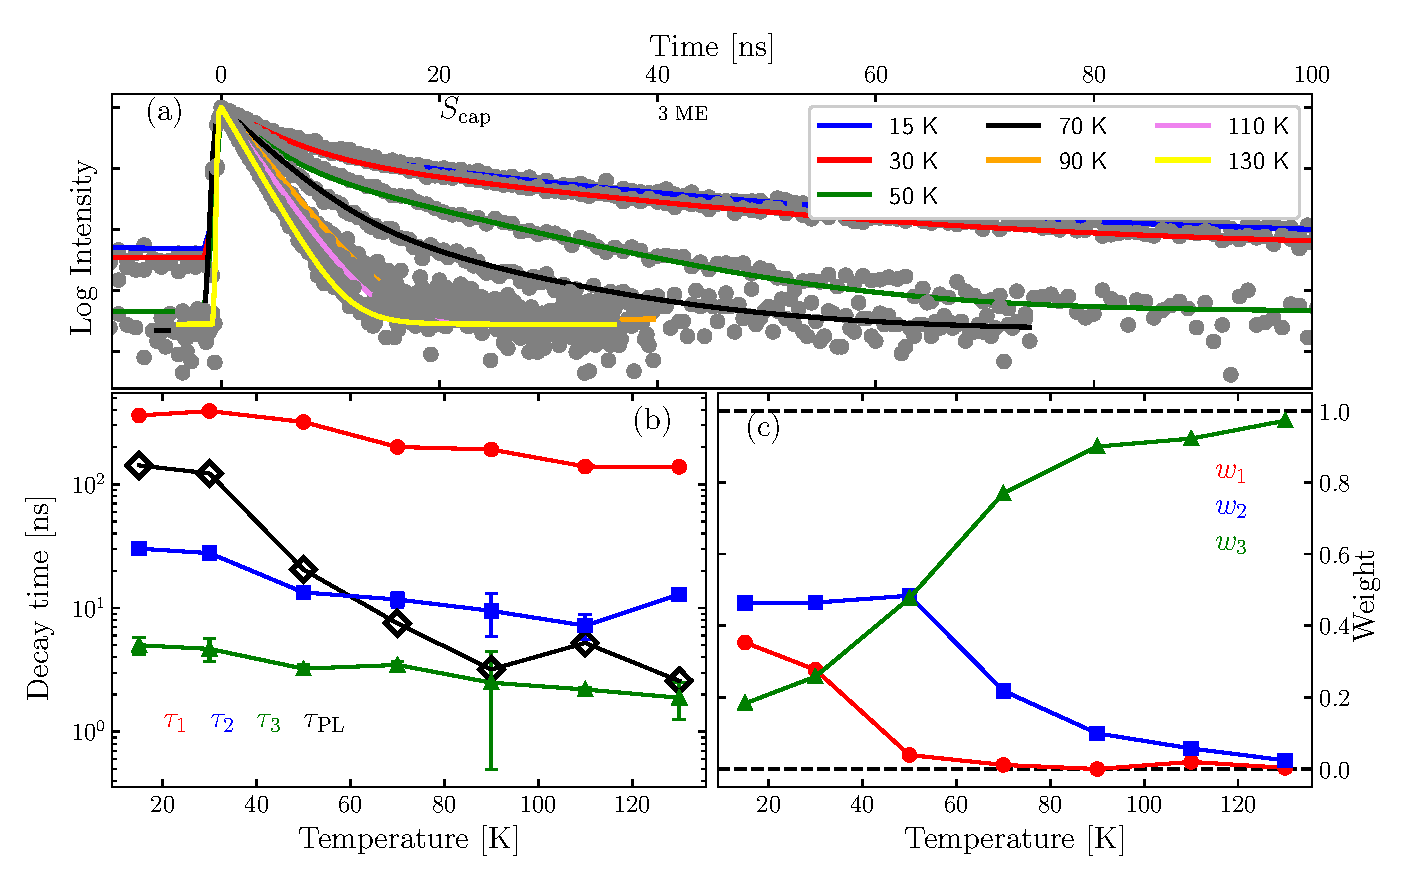
\includegraphics[width=0.9\linewidth]{/TRPL_after_Benito/temperature/12021_TRPL_700nm_temp}
	\caption{(a) Experimental TRPL at pumping power of 0.3~W/cm$^2$ as a function of temperature (grey circles) and its deconvolution by 3ME model (solid lines) at the maximum (1.75~eV) of PL signal for sample $S_\mathrm{cap}$. (b) Deconvolved decay times ($\tau_1$: red circles; $\tau_2$: blue squares; $\tau_3$: green triangles) and characteristic time $\tau_\mathrm{PL}$ (black diamonds) as a function of temperature. Corresponding weights are shown in panel (c).}
	\label{fig:TRPL_temp_c}
\end{figure}
%

\noindent where $I_0$ and $I_\mathrm{PL}$ are the PL intensity at 15~K and that as a function of $T$, respectively. As can be seen in Fig.~\ref{fig:TRPL_temp_decon}, $\tau_\mathrm{NR}$ decreases with temperature as is usually the case for thermally activated processes. Thereafter, we fit the reduction of the parameter $\tau_\mathrm{NR}$ with temperature by the following model involving two non-radiative processes 
%
\begin{equation}
\frac{1}{\tau_\mathrm{NR}}=\frac{1}{\tau_\mathrm{NR}^1}\exp{\left(\frac{-E_1}{k_\mathrm{B}T}\right)} + \frac{1}{\tau_\mathrm{NR}^2}\exp{\left(\frac{-E_2}{k_\mathrm{B}T}\right)} \label{eq:nonradiative}
\end{equation}
characterized by activation energies $E_1$ and $E_2$ and time constants $\tau_\mathrm{NR}^1$ and $\tau_\mathrm{NR}^2$, respectively.
Conversely, $\tau_\mathrm{R}$ increases exponentially with temperature
%
\begin{equation}
\tau_\mathrm{R} = \tau_\mathrm{R}^0 + \tau_\mathrm{R}^T \exp{\left(\frac{T}{T_C}\right)}, \label{eq:tau_R} 
\end{equation}
where $ \tau_\mathrm{R}^0$ ($ \tau_\mathrm{R}^T$) describes the temperature independent (dependent) part of the radiative decay and $T_C$ is the characteristic temperature corresponding to the energy of localized states. 

The behavior of the decay time of the fast component $\tau_2$ with temperature, on the other hand, suggests that there is a non-radiative contribution even at lowest temperatures which prevents using Eq.~(\ref{eq:tau_R_fromtau1}) directly. To overcome this limitation, we assume that the radiative lifetime at 15~K is the same that for the slow component $\tau_1$, $\tau_2^\mathrm{R}(15K)=\tau_1^\mathrm{R}(15K)$, and a temperature independent, non-radiative decay $\tau_\mathrm{C}$ is also present and that is given by
%
\begin{eqnarray}
\frac{1}{\tau_\mathrm{C}}=\frac{1}{\tau_2(15K)}-\frac{1}{\tau_2^\mathrm{R}(15K)}.\label{eq:tau_C}
\end{eqnarray}

Since $\tau_\mathrm{C}$ is temperature independent, we can now calculate the radiative lifetime $\tau_2^\mathrm{R}$ of the fast component at any temperature using Eq.~(\ref{eq:tau_R_fromtau1}) by replacing $\tau_1$ with $\tau_2$ and $1/\tau_\mathrm{NR}$ with $1/\tau_\mathrm{C}+1/\tau_2^\mathrm{NR}$. The overall decay time as a function of temperature will be given by:
\begin{eqnarray}
\frac{1}{\tau_2(T)}=\frac{1}{\tau_\mathrm{C}}+\frac{1}{\tau_2^\mathrm{R}(T)}+\frac{1}{\tau_2^\mathrm{NR}(T)}.
\end{eqnarray}
%
Now we can repeat the analysis of the radiative and non-radiative part described by Eqs.~(\ref{eq:tau_R})--(\ref{eq:nonradiative}) for $\tau_2^\mathrm{R}$ and $\tau_2^\mathrm{NR}$.

In the case of sample $S_\mathrm{cap}$ where three exponential decays are presented, we repeat the assumption described above for $\tau_3$ where we assumed the same radiative lifetime of $\tau_3$ as for $\tau_2$, $\tau_3^\mathrm{R}(15K)=\tau_2^\mathrm{R}(15K)$, and temperature independent non-radiative lifetime $\tau_\mathrm{C}$ similarly to Eq.~(\ref{eq:tau_C}) as $1 / \tau_\mathrm{C} = 1/ \tau_3(15K)-1/ \tau_3^\mathrm{R}(15K)$.

%KONEC PK
Combining Eq.~(\ref{eq:tau_R_fromtau1}) to Eq.~(\ref{eq:tau_R}) and repetition that for all decay times we can obtain an Arrhenius-like equation with an explicit dependence of the PL intensity on all the parameters derived from the TRPL analysis
%
\begin{equation}
I_\mathrm{PL}(T)=I_0\sum_{i=1}^{2(3)}\frac{1}{1+\left[\tau_{i\mathrm{R}}^0+\tau_{i\mathrm{R}}^T\exp{\left(\frac{T}{T_{i\mathrm{C}}}\right)}\right] \times \left[\frac{1}{\tau_{i\mathrm{NR}}^1}\exp{\left(\frac{-E_{i1}}{k_\mathrm{B}T}\right)} + \frac{1}{\tau_{i\mathrm{NR}}^2}\exp{\left(\frac{-E_{i2}}{k_\mathrm{B}T}\right)}\right]}, \label{eq:TRPL_Arhenius}
\end{equation}
%
where the upper limit of sum up depends on a number of mono-exponential decays in fitting model used for deconvolution of TRPL signal.
\begin{figure}
	\centering
	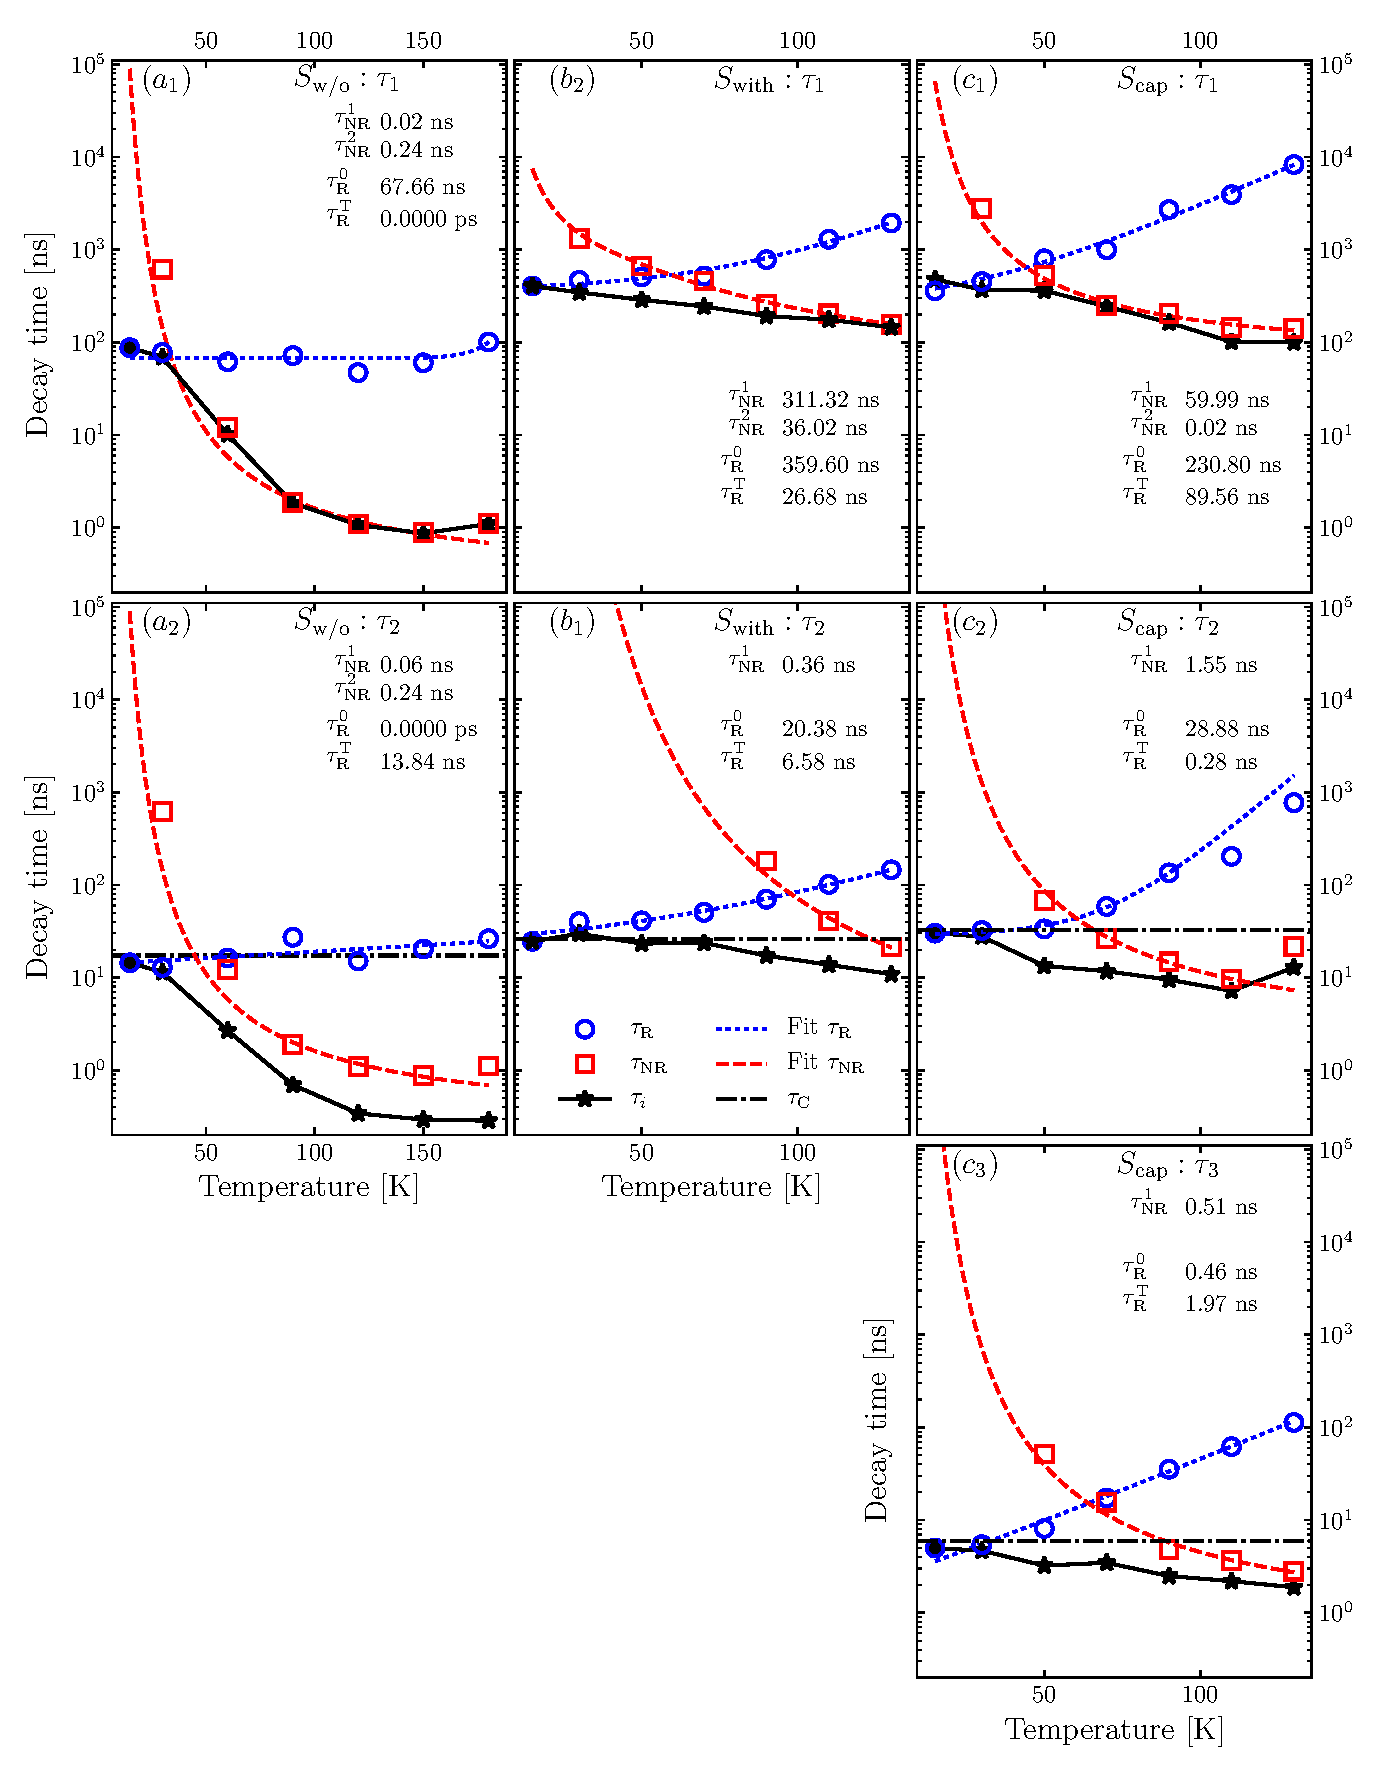
\includegraphics[width=1\linewidth]{/TRPL_after_Benito/temperature/decay_dekonvolution_all_after}
	\caption{Individual decay times $\tau_1$--$\tau_3$ as a function of temperature with the radiative and non-radiative components for all our samples - panels (a) show decay times for sample $S_\mathrm{w/o}$, (b) that for $S_\mathrm{with}$ and (c) for $S_\mathrm{cap}$. The radiative and non-radiative component are fitted by Eq.~(\ref{eq:tau_R}) and Eq.~(\ref{eq:nonradiative}), respectively.}
	\label{fig:TRPL_temp_decon}
\end{figure}

As it can be seen in Fig.~\ref{fig:Arrhenius_PLandTRPL}, this formula is equally good in reproducing experimental data as~Eq.~(\ref{eq:Arhenius}). 


\newpage

We now discuss the numerical results received in this analysis for individual decay times obtained from TRPL signal at maximum of PL intensity of each studied samples. The results are summarized in Tab.~\ref{tab:TRPL_params}. 

As can be seen in panels~(a$_1$) of Fig.~\ref{fig:TRPL_temp_decon} the radiative decay time of slow component $\tau_1$ of sample $S_\mathrm{w/o}$ does not depend on temperature, whereas radiative contribution of $\tau_2$ [panel (a$_2$)] enlarges exponentially with temperature from 0~ps at 0~K. This behaviour point to, that $\tau_2$ decay time is associated with phonon replica where in 0~K phonons are not available for assisted transition. With temperature amount of phonons increase resulting in increasing relevance of $\tau_2$ with temperature, see Fig.~\ref{fig:TRPL_temp_wo}~(c). To discuss non-radiative contribution, in both decay times we identified shallow impurities~\citep{Cardona} with localization energy $E_1$ around 16~meV and characteristic non-radiative constant $\tau^1_\mathrm{NR}$ of 235~ps. Activation energy $E_2=442-445$~meV of the second non-radiative process $\tau^2_\mathrm{NR}=20$~ps corresponds to unipolar scape of heavy holes from GaAs layer to GaP matrix. The obtained value of $E_2$ is in agreement with escape energy of {\color{green}{VALUE ještě jednou změřit v pythonu unikovou energii HH pro 5ML vrstvu}} determined from 8-band $\mathbf{k\cdot p}$ calculations.

\begin{table}
	\centering
	\caption{Summary of the TRPL Arrhenius-like fits. The displayed values are obtained with accuracy better than $10^{-3}\%$.}
	\begin{tabularx}{0.95\textwidth}{cCCccccc}
		\toprule
		
		& $E_1$ [meV]& $\tau_\mathrm{NR}^1$ [ns]& $E_2$ [meV]& $\tau_\mathrm{NR}^2$ [ns] & $\tau_\mathrm{R}^0$ [ns]& $\tau_\mathrm{R}^T$ [ns]& $T_C$ [K]\\ 	
		\midrule
		\midrule
		$S_\mathrm{w/o}$ $\tau_1$& 16.4&0.235&441.8 & 0.02& 67.66&0.00&8.21\\
		$S_\mathrm{w/o}$ $\tau_2$& 16.6&0.235&445.2 & 0.06& 0.00&13.84&311.2\\
		\midrule
		
		$S_\mathrm{with}$ $\tau_1$&4.10 & 311.3& 21.3&36.0& 359.6&26.68&31.7\\
		$S_\mathrm{with}$ $\tau_2$&45.5 & 0.36& --&--& 20.38&6.58&44.1\\
		\midrule
		
		$S_\mathrm{cap}$ $\tau_1$& 9.04&59.99&557.5 & 0.02& 230.8&89.56&28.9\\ %28.94
		$S_\mathrm{cap}$ $\tau_2$& 17.3&1.55&-- & --& 28.88&0.28&15.2\\ %15.18
		$S_\mathrm{cap}$ $\tau_3$& 18.73&0.51&-- & --& 0.456&1.97&31.9\\
		
		\bottomrule
	\end{tabularx}\label{tab:TRPL_params}
\end{table}

Looking to binding energy ($E=4-46$~meV) it seems that non-radiative losses of dynamical processes in $S_\mathrm{with}$ are caused by shallow traps. Contrary to radiative contribution in $S_\mathrm{w/o}$, we show in panels~(b$_1$)~and~(b$_2$) of Fig.~\ref{fig:TRPL_temp_decon} increasing of radiative part of both slow $\tau_1$ and as well as fast $\tau_2$ processes. The slower process starts at $\tau_\mathrm{R}^0=360$~ns and exponentially increasing proportional to $\tau_\mathrm{R}^T=26.68$~ns, whereas the faster process starts at 20.4~ns and is proportional to $\tau_\mathrm{R}^T=6.58$~ns. Energies of localized states of these two radiative times for $\tau_1$ and $\tau_2$ characterized by $T_\mathrm{C}$ are 31.7~K and 44.1~K, respectively.

In case of $S_\mathrm{cap}$ we can shown in panels~(c$_1$)--(c$_3$) similar behavior of radiative times of individual dynamics processes as in $S_\mathrm{with}$. Regardless different $\tau_\mathrm{R}^0=230.8$~ns and $\tau_\mathrm{R}^0=456$~ps at 0~K and dissimilar $\tau_\mathrm{R}^T=89.56$~ns and $\tau_\mathrm{R}^T=1.97$~ns for $\tau_1$ and $\tau_3$ processes, respectively, we found comparable values of $T_\mathrm{C}$ for that which lead us to an opinion that these processes come from same structure. This ascertainment is in agreement with the result from SSCCI calculations presented in the previous section, where $\tau_1$ was identified as transition between electrons from $L$ and holes from $\Gamma$-point and $\tau_3$ as transition from $\Gamma$ electrons. From analysis of non-radiative times we found escape localization energy of electrons from $\Gamma$-point of $E_2=557.5$~meV which is comparable to $400$~meV calculated by 8-band $\mathbf{k \cdot p}$ method. Other non-radiative processes are in the range of localization energies of shallow traps.

% KONEC PS

%The non-radiative process with smaller activation energy ($E_1$ between 6 and 18~meV) is probably associated with trapping of carriers by impurities or defects in the vicinity of QDs, as it has been also before for InAs/InP quantum wires~\citep{Alen_apl2011}. The other process is characterized by faster time constant $\tau_\mathrm{NR}^2$ ($\tau_\mathrm{NR}^1/\tau_\mathrm{NR}^2>5$) is close to the thermally activated capture of excitions by nonradiative defects in GaAs layer~\citep{Seravallo_apl2005,Kohki_apl1997}. 

The values obtained by fitting the dependencies by model in Eq.~(\ref{eq:TRPL_Arhenius}) are summarized in Tab.~\ref{tab:TRPL_params} and are comparable with parameters gained from the temperature dependence of integrated PL intensity shown in Sec.~\ref{Sec:temp_PL_TU}, which are equally well reproduced by Eq.~(\ref{eq:Arhenius}), see the parameters resume in Tab.~\ref{tab:Arhenius}.

The previous temperature dependent TRPL and PL analysis of our samples allow us to draw simple scheme of the time evolution of the levels involved in the exciton dynamics, namely that of the recombining level \textbf{F} and trap levels, see Fig.~\ref{fig:Arrhenius_PLandTRPL}. The escape energies of carriers from the structure to the matrix \textbf{G} are also added into that. 


\section{Comparison theoretical models with experimental results} \label{sec:TUB_results}

\begin{figure}
	\centering
	\includegraphics[width=0.9\linewidth]{/TRPL_after_Benito/temperature/models_v2} %Arrhenius_PLandTRPL_all}
	\caption{The left panels (a)-(c) compare the integrated PL intensity and the corresponding Arhenius fit for all our samples of the measurements performed with a CW (circles) and a pulsed (squares) laser. The right panels show levels involved in the exciton dynamics in our samples. The letters \textbf{0} and \textbf{F} in these sketches represent the vacuum end exciton state, respectively, \textbf{G} is escape energy of carriers from structure to the bulk matrix.}
	\label{fig:Arrhenius_PLandTRPL}
\end{figure}
\newpage 


\begin{figure}
	\centering
	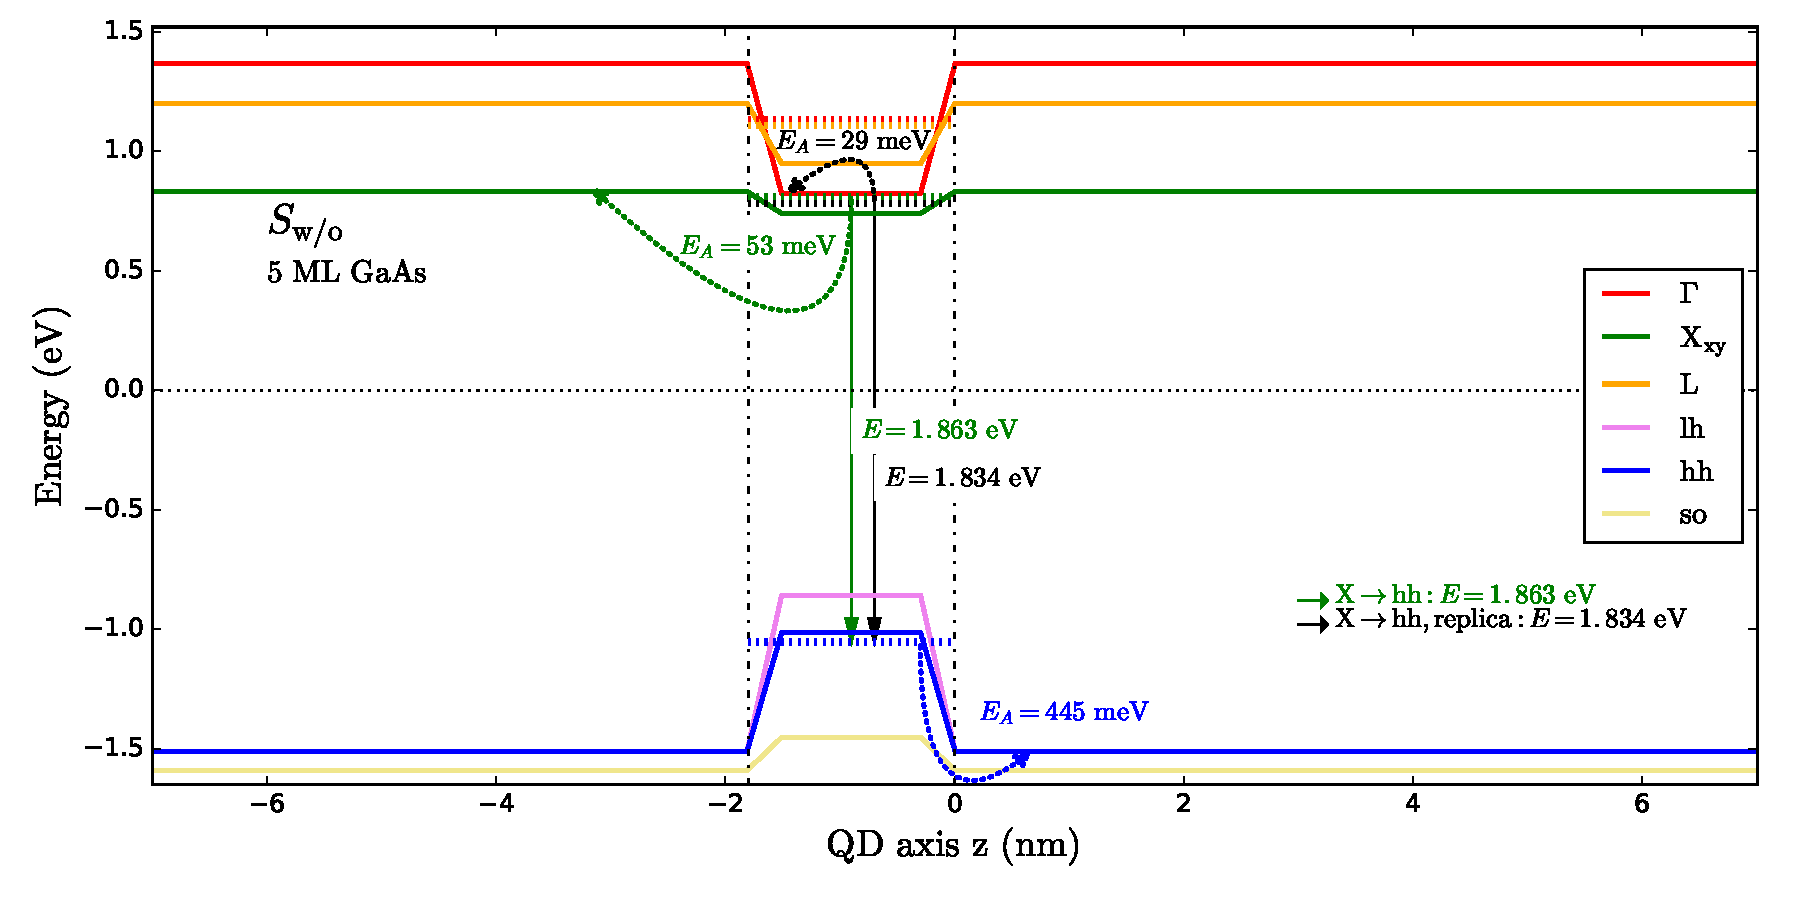
\includegraphics[width=0.9\linewidth]{/band_scheme/Eli_15nm_5ML_Ga05_As_0_banddiagram} %Arrhenius_PLandTRPL_all}
	\caption{}
	\label{fig:Band_scheme_wo}
\end{figure}


\begin{figure}
	\centering
	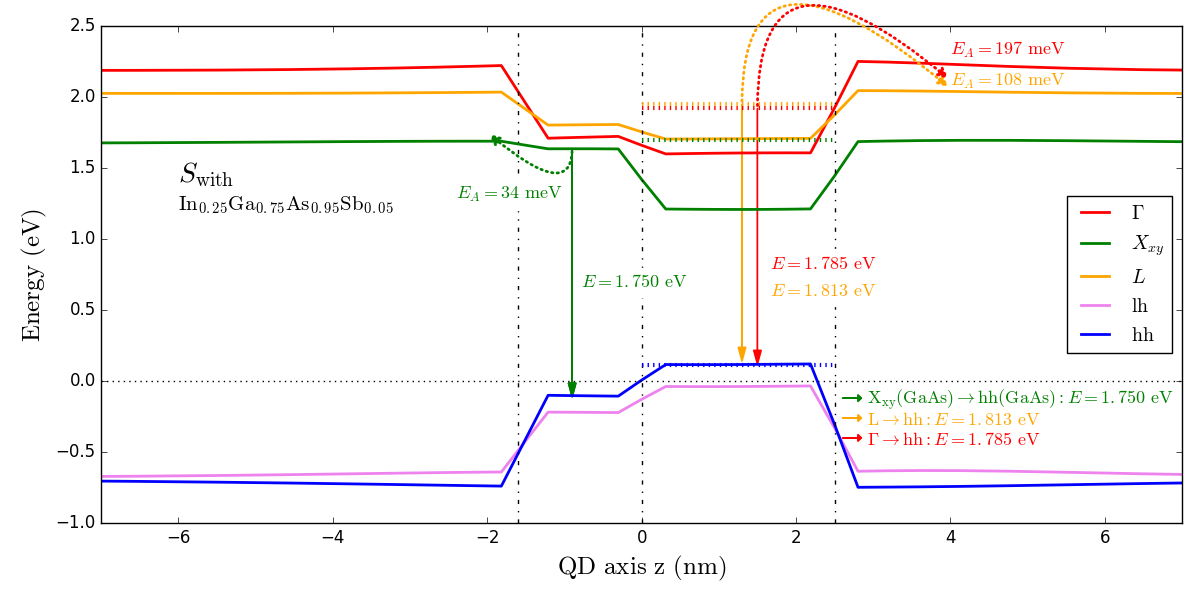
\includegraphics[width=0.9\linewidth]{/band_scheme/Ga75A95}%Arrhenius_PLandTRPL_all}
	\caption{}
	\label{fig:Band_scheme_with}
\end{figure}

\begin{figure}
	\centering
	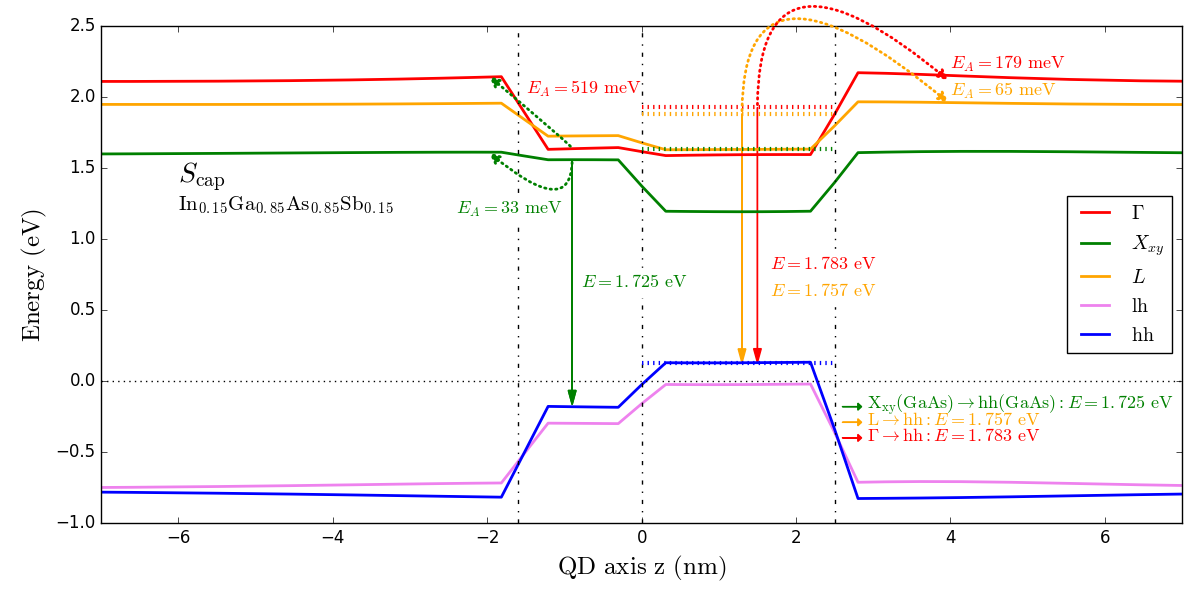
\includegraphics[width=0.9\linewidth]{/band_scheme/Ga85A85}%Arrhenius_PLandTRPL_all}
	\caption{}
	\label{fig:Band_scheme_cap}
\end{figure}

\section{Conclusions}
We have experimentally studied the electronic structure of set (without QDs, with QDs, with QDs and GaSb capping) of In$_{1-x}$Ga$_{x}$As$_y$Sb$_{1-y}$/GaP QDs with 5~ML GaAs interlayer grown by MOVPE. We have pointed by TEM and EDX measurements to a high amount of Ga and As in our samples which lead to type-I band alignment. Furthermore, we have shown that the samples emitted around 1.8~eV with anisotropy elongated along [110]~crystallographic direction.   % For our analysis set of sample (without QDs, with QDs, with QDs and GaSb capping) were grown by MOVPE. 

{\color{green}{Podívej se i zpět do textu, přibyly tam modre podbarvene texty
	
	Zmínit, že se povedlo narůst 5ML GaAs vrstvu}} {\color{red}{CO DÁL???}}